\documentclass[12pt,a4paper]{article}
\usepackage[utf8]{inputenc}
\usepackage[T5]{fontenc}
\usepackage[vietnamese]{babel}
\usepackage{mathptmx}           % Times New Roman font
\usepackage{geometry}
\geometry{top=2cm, bottom=2cm, left=2.5cm, right=2cm, headheight=14.5pt}
\usepackage{longtable}
\usepackage{array}
\usepackage{amssymb}
\usepackage{indentfirst}
\usepackage{booktabs}
\usepackage{xcolor}
\usepackage{colortbl}
\usepackage{enumitem}
\usepackage{graphicx}
\usepackage{float}
\usepackage{fancyhdr}
\usepackage{lastpage}
\usepackage{tikz}
\usetikzlibrary{calc}

% --- Cấu hình đường dẫn ảnh ---
\graphicspath{{../images/}}

\definecolor{headerblue}{RGB}{220,230,242}
\definecolor{notegreen}{RGB}{234,250,234}

% --- Cấu hình Header & Footer ---
\pagestyle{fancy}
\fancyhf{}
\fancyhead[L]{\small \leftmark}
\fancyhead[R]{\small Trang \thepage/\pageref{LastPage}}
\renewcommand{\headrulewidth}{0.4pt}
\renewcommand{\sectionmark}[1]{\markboth{#1}{}}
\setcounter{tocdepth}{3}
\setcounter{secnumdepth}{3}

\begin{document}

\begin{titlepage}
    \newgeometry{left=2cm, right=2cm, top=2cm, bottom=2cm}
    \begin{tikzpicture}[remember picture, overlay]
        \draw[line width = 2pt] ($(current page.north west) + (1.5cm,-1.5cm)$) rectangle ($(current page.south east) + (-1.5cm,1.5cm)$);
        \draw[line width = 0.5pt] ($(current page.north west) + (1.6cm,-1.6cm)$) rectangle ($(current page.south east) + (-1.6cm,1.6cm)$);
    \end{tikzpicture}

    \begin{center}
        \large \textbf{HỌC VIỆN CÔNG NGHỆ BƯU CHÍNH VIỄN THÔNG} \\
        \large \textbf{KHOA CÔNG NGHỆ THÔNG TIN 2} \\
        \large \textbf{BỘ MÔN THỰC TẬP CƠ SỞ} \\
        \vspace{0.5cm}
        \rule{3cm}{1pt} \\

        \vspace{1.2cm}
        
\includegraphics[width=5.5cm]{Logo_PTIT_University.png} \\
        \vspace{1.5cm}

        \LARGE \textbf{BÁO CÁO CUỐI KỲ} \\
        \vspace{0.5cm}
        \Large \textbf{PHÂN TÍCH VÀ XÁC ĐỊNH YÊU CẦU HỆ THỐNG} \\
        \vspace{1cm}

        \begin{minipage}{14cm}
            \centering
            \large \textbf{Đề tài: Hệ thống nhận diện bệnh trên cây lúa dựa trên thuật toán học sâu CNN}
        \end{minipage}

        \vspace{2.5cm}

        \begin{tabular}{l l}
            \textbf{Giảng viên hướng dẫn:} & Cô Nguyễn Thị Bích Nguyên           \\
            \textbf{Nhóm:}                 & Nhóm 1                              \\
            \textbf{Lớp:}                  & E23CQCE01-N                         \\
            \textbf{Sinh viên thực hiện:}  & 1. Phan Tuấn Quốc Anh - N23DCCN003  \\
                                           & 2. Phạm Minh Khang - N23DCAT034     \\
                                           & 3. Nguyễn Lê Minh Phúc - N23DCDK058 \\
        \end{tabular}

        \vfill
        \large \textbf{TP. HỒ CHÍ MINH - 2026}
    \end{center}
    \restoregeometry
\end{titlepage}

\clearpage
\tableofcontents
\clearpage
\listoffigures
\clearpage
\listoftables
\clearpage

% ============================================================
\section{Tầm nhìn dự án}

\begin{longtable}{|l|p{11.5cm}|}
    \caption{Tầm nhìn dự án}                                                                                                                                 \\
    \hline
    \rowcolor{headerblue}
    \textbf{Mục}               & \textbf{Nội dung}                                                                                                           \\
    \hline
    \textbf{Nỗi đau hiện tại}  & Chẩn đoán bệnh trên cây lúa bằng mắt thường dẫn đến kết quả sai lệch, xử lý chậm trễ (1--3 ngày) và lạm dụng thuốc hóa học. \\
    \hline
    \textbf{Giải pháp đề xuất} & Ứng dụng trí tuệ nhân tạo (CNN) nhận diện bệnh qua hình ảnh, kết hợp dữ liệu thời tiết (GPS) và gợi ý dinh dưỡng thực vật.  \\
    \hline
    \textbf{Giá trị mang lại}  & Chẩn đoán nhanh (5--7 giây), chính xác, giảm phụ thuộc thuốc hóa học, nâng cao năng suất nông nghiệp.                       \\
    \hline
    \textbf{Ngoài phạm vi}     & Cảm biến IoT, thương mại điện tử, tích hợp ERP doanh nghiệp.                                                                \\
    \hline
\end{longtable}

% ============================================================
\section{Quy trình hiện tại và quy trình đề xuất}

\textbf{Quy trình hiện tại (As-Is):}
\begin{enumerate}
    \item Nông dân phát hiện triệu chứng bất thường trên lá lúa.
    \item Tự đoán bệnh dựa trên kinh nghiệm hoặc hỏi người xung quanh (mất 1--3 ngày).
    \item Mua thuốc bảo vệ thực vật theo cảm tính, dễ lạm dụng hóa chất.
\end{enumerate}

\textbf{Quy trình đề xuất (To-Be):}
\begin{enumerate}
    \item Nông dân chụp ảnh lá lúa bằng điện thoại.
    \item Hệ thống AI nhận diện bệnh trong 5--7 giây, khoanh vùng bệnh trên ảnh.
    \item Hệ thống gợi ý dinh dưỡng phù hợp với loại bệnh được phát hiện.
    \item Nông dân có thể phản hồi nếu kết quả chưa chính xác.
    \item Dữ liệu phản hồi được dùng để tái huấn luyện và nâng cấp mô hình AI.
\end{enumerate}

\hrulefill

% ============================================================
\section{Phạm vi áp dụng đề tài}
\begin{itemize}
    \item \textbf{Phạm vi nghiệp vụ:} Hệ thống số hóa quy trình chẩn đoán bệnh lúa qua hình ảnh bằng công nghệ nhận diện chuyên sâu. Hệ thống kết hợp phân tích hình ảnh và các thông số môi trường để đưa ra chẩn đoán chính xác. Kết hợp xây dựng kho tri thức về dinh dưỡng thực vật để gợi ý các loại vitamin và vi lượng cần bổ sung dựa trên việc truy xuất dữ liệu thông minh.
    \item \textbf{Phạm vi đối tượng:} Phục vụ Nông dân (nhận diện \& nhận gợi ý dinh dưỡng) và Quản trị viên (quản lý danh mục, cập nhật mô hình, quản lý kho kiến thức hệ thống).
    \item \textbf{Giới hạn đề tài:} Hệ thống tự chủ kho dữ liệu dinh dưỡng nội bộ. Đối với thông số môi trường, hệ thống sử dụng tọa độ vị trí (GPS) để tự động truy xuất dữ liệu thời tiết làm dữ liệu phụ trợ. Hỗ trợ nhận diện nhiều loại bệnh cùng lúc trên cùng một ảnh.
\end{itemize}

% ============================================================
\section{Các bước xác định yêu cầu}

Quá trình thực hiện xác định yêu cầu gồm 2 bước chính như sau:
\begin{itemize}
    \item \textbf{Bước 1:} Khảo sát hiện trạng, kết quả nhận được là các báo cáo về hiện trạng chẩn đoán bệnh trên cây lúa và nhu cầu bổ sung dinh dưỡng.
    \item \textbf{Bước 2:} Lập danh sách các yêu cầu, kết quả nhận được là danh sách các yêu cầu sẽ được thực hiện trên hệ thống máy tính.
\end{itemize}

\subsection{Đối tượng tham gia xác định yêu cầu}
Gồm 2 nhóm người:
\begin{itemize}
    \item \textbf{Chuyên viên tin học:} Thiết kế kiến trúc nhận diện thông minh, xây dựng kho kiến thức hệ thống và luồng xử lý truy xuất thông tin dinh dưỡng chính xác nhất.
    \item \textbf{Nhà chuyên môn (Kỹ sư nông nghiệp):} Cung cấp dữ liệu ảnh kèm thông số môi trường tương ứng, gán nhãn bệnh và trực tiếp biên soạn/chuẩn hóa bộ dữ liệu văn bản về vitamin/dinh dưỡng.
\end{itemize}
Hai nhóm người này phối hợp thật chặt chẽ để có thể xác định đầy đủ và chính xác các yêu cầu.

\hrulefill

\subsection{Khảo sát hiện trạng}
% ============================================================
% DANH SÁCH BỆNH LÚA TRONG ĐỀ TÀI
% ============================================================
\subsection{Danh sách và mô tả các bệnh lúa trong đề tài}
Hệ thống được xây dựng để nhận diện 5 loại bệnh phổ biến trên cây lúa tại Việt Nam và khu vực Đông Nam Á. Thông tin về từng bệnh được tổng hợp từ tài liệu của Viện Lúa Quốc tế (IRRI) và các nghiên cứu chuyên ngành nông nghiệp.

\vspace{0.3cm}

\begin{longtable}{|
    >{\raggedright\arraybackslash}p{2.5cm}|
    >{\raggedright\arraybackslash}p{3cm}|
    >{\raggedright\arraybackslash}p{2cm}|
    >{\raggedright\arraybackslash}p{4cm}|
    >{\raggedright\arraybackslash}p{3cm}|}
    
% --- 1. Tiêu đề và Đầu bảng (Trang đầu tiên) ---
\caption{Danh sách và mô tả 5 bệnh lúa trong đề tài}
\label{tab:diseases} \\
\hline
\rowcolor{headerblue}
\textbf{Tên bệnh} & \textbf{Tác nhân gây bệnh} & \textbf{Giai đoạn ảnh hưởng} & \textbf{Triệu chứng đặc trưng} & \textbf{Điều kiện phát sinh} \\ \hline
\endfirsthead

% --- 2. Đầu bảng (Cho các trang tiếp theo nếu bảng bị ngắt) ---
\multicolumn{5}{c}%
{{\tablename\ \thetable{} -- Tiếp theo trang trước}} \\
\hline
\rowcolor{headerblue}
\textbf{Tên bệnh} & \textbf{Tác nhân gây bệnh} & \textbf{Giai đoạn ảnh hưởng} & \textbf{Triệu chứng đặc trưng} & \textbf{Điều kiện phát sinh} \\ \hline
\endhead

% --- 3. Chân bảng (Cho các trang giữa nếu bảng bị ngắt) ---
\hline \multicolumn{5}{|r|}{{Tiếp tục ở trang sau...}} \\ \hline
\endfoot

% --- 4. Chân bảng (Trang cuối cùng của bảng) ---
\hline
\endlastfoot

% ==========================================
% NỘI DUNG BẢNG
% ==========================================

\textbf{Bạc lá} \newline \textit{Bacterial Blight} & 
Vi khuẩn \textit{Xanthomonas oryzae} pv.\ \textit{oryzae} & 
Mạ đến trỗ bông & 
Lá non chuyển xanh xám và cuộn lại. Ở cây lớn, xuất hiện các vết sọc vàng cam dọc mép lá hoặc đầu lá, lan rộng dần thành màu vàng rơm và khô trắng. Mủ vi khuẩn màu vàng chảy ra khi cắt ngang phần bị bệnh. & 
Độ ẩm $>$ 70\%, nhiệt độ 25--34$^\circ$C, gió mạnh và mưa liên tục, bón thừa đạm. \\ \hline 

\textbf{Đốm nâu} \newline \textit{Brown Spot} & 
Nấm \textit{Bipolaris oryzae} & 
Mạ đến chín sữa & 
Xuất hiện các đốm tròn hoặc bầu dục màu nâu trên lá, có tâm xám và viền đỏ nâu đặc trưng. Đốm có thể liên kết với nhau gây cháy toàn bộ lá. Hạt bị nhiễm có vết đen hoặc đổi màu (``pecky rice''). & 
Độ ẩm 86--100\%, nhiệt độ 16--36$^\circ$C, lá ẩm liên tục 8--24 giờ, đất thiếu dinh dưỡng (đặc biệt là kali và silic). \\ \hline 

\textbf{Đạo ôn} \newline \textit{Rice Blast} & 
Nấm \textit{Magnaporthe oryzae} & 
Mạ đến trỗ bông & 
Vết bệnh hình thoi hoặc hình mắt én trên lá, tâm xám trắng, viền nâu đỏ, có quầng vàng xung quanh. Ở cổ bông (cổ cháy) gây lép hạt hàng loạt. Có thể giết chết cây ở giai đoạn mạ. & 
Độ ẩm $>$ 90\%, nhiệt độ ban ngày 25--28$^\circ$C và ban đêm 17--23$^\circ$C, sương mù buổi sáng, bón thừa đạm. \\ \hline 

\textbf{Vàng lùn lúa cỏ} \newline \textit{Rice Tungro} & 
2 loại virus: \textit{Rice tungro bacilliform virus} (RTBV) và \textit{Rice tungro spherical virus} (RTSV), lây truyền qua rầy xanh \textit{Nephotettix virescens} & 
Đẻ nhánh đến làm đòng & 
Lá chuyển màu vàng hoặc vàng cam từ đầu lá lan vào. Cây còi cọc, thấp lùn, đẻ nhánh ít. Bông nhỏ, trỗ không thoát, hạt lép nhiều và có đốm nâu. & 
Nhiệt độ 25--35$^\circ$C, độ ẩm cao, mật độ rầy xanh lớn trên đồng. Rầy chỉ cần hút nhựa cây bệnh trong 5 phút là có thể truyền virus. \\ \hline 

\textbf{Khô vằn} \newline \textit{Sheath Blight} & 
Nấm \textit{Rhizoctonia solani} & 
Đẻ nhánh đến chín sữa & 
Vết bệnh hình bầu dục hoặc không đều trên bẹ lá, ban đầu màu xanh xám ngấm nước, sau chuyển xám trắng với viền nâu. Bệnh lan từ bẹ lên phiến lá và sang các nhánh lân cận. Có thể tìm thấy hạch nấm (sclerotia) màu nâu trên vết bệnh. & 
Độ ẩm 85--100\%, nhiệt độ 28--32$^\circ$C, mùa mưa, mật độ sạ dày, ruộng ngập nước. \\

\end{longtable}
\subsubsection{Các hình thức thực hiện phổ biến}
\begin{itemize}
    \item \textbf{Quan sát:} Theo dõi và ghi hình quá trình cây lúa biểu hiện triệu chứng thiếu hụt dinh dưỡng hoặc mắc nhiều bệnh cùng lúc trên đồng ruộng dưới các điều kiện thời tiết khác nhau.
    \item \textbf{Khảo sát:} Khảo sát các người nông dân về mối liên hệ giữa các loại bệnh lúa, sự thiếu hụt dinh dưỡng và sự tác động của môi trường (nhiệt độ, độ ẩm).
    \item \textbf{Thu thập thông tin, tài liệu:} Thu thập tập dữ liệu ảnh lá lúa (kèm dữ liệu đặc tả về thời tiết/độ ẩm) và chuẩn bị bộ dữ liệu văn bản về dinh dưỡng thực vật.
\end{itemize}

\subsubsection{Quy trình thực hiện}
\textbf{A. Tìm hiểu tổng quan về thế giới thực:}
\begin{itemize}
    \item Quy mô hoạt động nông nghiệp, các bệnh dịch thường gặp.
    \item Xu hướng chuyển dịch sang bổ sung vitamin tăng sức đề kháng thay vì lạm dụng thuốc hóa học.
\end{itemize}

\textbf{B. Tìm hiểu hiện trạng tổ chức (cơ cấu tổ chức):}
\begin{itemize}
    \item Cơ cấu tổ chức bao gồm các chức danh: Quản trị viên (Quản lý dữ liệu bệnh, mô hình, tập dữ liệu dinh dưỡng), Nông dân (tải ảnh và mô tả tình trạng).
\end{itemize}

\textbf{C. Tìm hiểu hiện trạng nghiệp vụ:}
\begin{itemize}
    \item Việc tìm hiểu dựa trên: Thông tin đầu vào, Quá trình xử lý, Thông tin kết xuất.
    \item Xếp loại các nghiệp vụ vào 4 loại: Lưu trữ, Tính toán, Tra cứu, Kết xuất.
\end{itemize}

\hrulefill

\subsection{Lập danh sách các yêu cầu}
\subsubsection{Xác định yêu cầu chức năng nghiệp vụ}

% ============================================================
% NGƯỜI DÙNG: NÔNG DÂN
% ============================================================
\section{Người dùng --- Nông dân (Mã số: ND)}
 
\textbf{Định nghĩa:} Người sử dụng hệ thống với mục đích chẩn đoán bệnh trên cây lúa qua hình ảnh, xem gợi ý dinh dưỡng và phản hồi kết quả chẩn đoán.
 
\vspace{0.3cm}
\textbf{1. Bảng yêu cầu chức năng nghiệp vụ}
 
\begin{longtable}{|
        c|
        >{\raggedright\arraybackslash}p{3.2cm}|
        >{\raggedright\arraybackslash}p{2.2cm}|
        >{\raggedright\arraybackslash}p{2.4cm}|
        >{\raggedright\arraybackslash}p{2.6cm}|
        >{\raggedright\arraybackslash}p{2.6cm}|}
    \hline
    \rowcolor{headerblue}
    \textbf{STT} & \textbf{Công việc}               & \textbf{Loại công việc} & \textbf{Quy định/CT liên quan} & \textbf{Biểu mẫu liên quan} & \textbf{Ghi chú}         \\
    \hline
    \endhead
    \multicolumn{6}{|l|}{\cellcolor{notegreen}\textbf{I. Quản lý tài khoản}}                                                                                            \\
    \hline
    1            & Đăng ký tài khoản                & Lưu trữ                 & QĐ-ND-01                       & ND\_BM 1                    &                          \\
    \hline
    2            & Đăng nhập hệ thống               & Tra cứu                 & QĐ-ND-01                       & ND\_BM 1b                   &                          \\
    \hline
    3            & Khôi phục mật khẩu               & Lưu trữ                 & QĐ-ND-01                       &                             &                          \\
    \hline
    4            & Đổi mật khẩu                     & Lưu trữ                 & QĐ-ND-01                       & ND\_BM 1c                   &                          \\
    \hline
    5            & Đăng xuất hệ thống               & Lưu trữ                 & QĐ-ND-01                       &                             &                          \\
    \hline
    \multicolumn{6}{|l|}{\cellcolor{notegreen}\textbf{II. Hồ sơ cá nhân}}                                                                                               \\
    \hline
    6            & Xem thông tin cá nhân            & Tra cứu                 & QĐ-ND-02                       &                             &                          \\
    \hline
    7            & Chỉnh sửa thông tin cá nhân      & Lưu trữ                 & QĐ-ND-02                       & ND\_BM 2                    &                          \\
    \hline
    \multicolumn{6}{|l|}{\cellcolor{notegreen}\textbf{III. Chẩn đoán bệnh lúa}}                                                                                         \\
    \hline
    8            & Gửi ảnh chẩn đoán                & Lưu trữ                 & QĐ-ND-03a                      & ND\_BM 3                    &                          \\
    \hline
    9            & Nhập vị trí ruộng                & Lưu trữ                 & QĐ-ND-03b                      &                             & Tùy chọn, không bắt buộc \\
    \hline
    10           & Mô tả triệu chứng                & Lưu trữ                 & QĐ-ND-03c                      &                             & Tùy chọn, không bắt buộc \\
    \hline
    11           & Nhập thông số thực địa           & Lưu trữ                 & QĐ-ND-03d                      & ND\_BM 3b                   & Tùy chọn, không bắt buộc \\
    \hline
    12           & Xem kết quả chẩn đoán            & Tra cứu, Tính toán      & QĐ-ND-03e                      &                             &                          \\
    \hline
    \multicolumn{6}{|l|}{\cellcolor{notegreen}\textbf{IV. Tra cứu \& Phản hồi}}                                                                                         \\
    \hline
    13           & Tra cứu lịch sử chẩn đoán        & Tra cứu                 & QĐ-ND-04                       &                             &                          \\
    \hline
    14           & Xem chi tiết một lần chẩn đoán   & Tra cứu                 & QĐ-ND-04                       &                             &                          \\
    \hline
    15           & Gửi phản hồi kết quả             & Lưu trữ                 & QĐ-ND-05                       & ND\_BM 4                    &                          \\
    \hline
    16           & Xem kết quả xử lý phản hồi       & Tra cứu                 & QĐ-ND-05                       &                             &                          \\
    \hline
\end{longtable}
 
% ============================================================
\vspace{0.3cm}
\textbf{2. Bảng Quy định / Công thức liên quan --- Nông dân}
 
% ---- QĐ-ND-01 ----
\vspace{0.3cm}
\noindent\textbf{QĐ-ND-01 --- Quy định Tài khoản}
 
\begin{longtable}{|
    >{\raggedright\arraybackslash}p{2.8cm}|
    >{\raggedright\arraybackslash}p{12cm}|}
\hline
\rowcolor{headerblue}
\textbf{Chức năng} & \textbf{Quy trình \& Ràng buộc} \\
\hline
\endhead
\textbf{a) Đăng ký tài khoản} &
Nông dân phải cung cấp đầy đủ các thông tin sau:
\begin{itemize}[leftmargin=*,topsep=2pt,itemsep=1pt]
    \item \textbf{Tên đăng nhập:} phải là duy nhất trong hệ thống, không chứa khoảng trắng, chỉ gồm chữ cái, chữ số và dấu gạch dưới.
    \item \textbf{Email:} đúng định dạng email, chưa tồn tại trong hệ thống.
    \item \textbf{Mật khẩu:} tối thiểu 8 ký tự, bao gồm ít nhất 1 chữ cái viết hoa, 1 chữ số và 1 ký tự đặc biệt.
    \item \textbf{Xác nhận mật khẩu:} phải gõ lại chính xác giống mật khẩu đã nhập.
\end{itemize}
Hệ thống gửi liên kết xác thực hoặc mã OTP về email để kích hoạt tài khoản. \\
\textbf{Quy tắc xử lý:} Sau khi đăng ký thành công, hệ thống tự động chuyển nông dân tới trang đăng nhập. \\
\hline
\textbf{b) Đăng nhập} &
Nông dân phải nhập đầy đủ 2 thông tin sau (không được để trống):
\begin{itemize}[leftmargin=*,topsep=2pt,itemsep=1pt]
    \item \textbf{Tên đăng nhập hoặc Email:} phải tồn tại trong hệ thống.
    \item \textbf{Mật khẩu:} phải khớp với tài khoản tương ứng.
\end{itemize}
\textbf{Cơ chế bảo mật:} Nếu đăng nhập sai, hệ thống chỉ hiển thị thông báo chung ``Tên đăng nhập hoặc mật khẩu không chính xác'' mà không chỉ rõ trường nào sai. Nếu đăng nhập sai quá 5 lần liên tiếp, hệ thống tạm khóa tài khoản trong 15 phút. Hệ thống cấp chứng chỉ phiên làm việc (JWT) sau khi xác thực thành công. \\
\textbf{Quy tắc xử lý:} Sau khi đăng nhập thành công, hệ thống tự động chuyển nông dân tới trang chẩn đoán bệnh. \\
\hline
\textbf{c) Khôi phục mật khẩu} &
Thực hiện theo 4 bước tuần tự:
\begin{enumerate}[leftmargin=*,topsep=2pt,itemsep=1pt]
    \item Nhập \textbf{địa chỉ email} đã đăng ký trong hệ thống.
    \item Hệ thống gửi \textbf{mã OTP} 6 chữ số về email --- hiệu lực 10 phút. Nhập sai 3 lần thì hủy mã.
    \item Nhập \textbf{mật khẩu mới} --- không được trùng mật khẩu cũ, đáp ứng độ mạnh như khi đăng ký.
    \item Nhập \textbf{xác nhận mật khẩu mới} --- phải gõ chính xác giống bước 3.
\end{enumerate}
\textbf{Quy tắc xử lý:} Sau khi đặt lại mật khẩu thành công, hệ thống tự động hủy tất cả phiên đăng nhập cũ trên các thiết bị khác và chuyển nông dân về trang đăng nhập. \\
\hline
\textbf{d) Đổi mật khẩu} &
Thực hiện theo các bước sau:
\begin{enumerate}[leftmargin=*,topsep=2pt,itemsep=1pt]
    \item Nông dân chọn chức năng Đổi mật khẩu trong hồ sơ cá nhân.
    \item Nhập \textbf{mật khẩu hiện tại} để hệ thống xác thực.
    \item Nhập \textbf{mật khẩu mới} --- đáp ứng độ mạnh (tối thiểu 8 ký tự, gồm chữ hoa, chữ số và ký tự đặc biệt) và không được trùng mật khẩu cũ.
    \item Nhập \textbf{xác nhận mật khẩu mới} --- phải gõ chính xác giống bước 3.
\end{enumerate}
\textbf{Quy tắc xử lý:} Hệ thống cập nhật mật khẩu mới và tự động hủy các phiên đăng nhập đang tồn tại trên các thiết bị khác. \\
\hline
\textbf{e) Đăng xuất} &
\begin{enumerate}[leftmargin=*,topsep=2pt,itemsep=1pt]
    \item Nông dân nhấn nút Đăng xuất trên giao diện.
    \item Hệ thống lập tức chấm dứt phiên làm việc hiện tại.
    \item Hệ thống xóa bộ nhớ đệm trên trình duyệt và chuyển hướng nông dân về màn hình Đăng nhập.
\end{enumerate} \\
\hline
\end{longtable}
 
% ---- QĐ-ND-02 ----
\vspace{0.3cm}
\noindent\textbf{QĐ-ND-02 --- Quy định Hồ sơ cá nhân}
 
\begin{longtable}{|
    >{\raggedright\arraybackslash}p{2.8cm}|
    >{\raggedright\arraybackslash}p{12cm}|}
\hline
\rowcolor{headerblue}
\textbf{Chức năng} & \textbf{Quy trình \& Ràng buộc} \\
\hline
\endhead
\textbf{a) Xem thông tin cá nhân} &
Nông dân chỉ xem được thông tin của chính mình sau khi đã đăng nhập. Thông tin hiển thị gồm: tên đăng nhập, họ tên, địa chỉ email, vị trí GPS và ngày tham gia hệ thống. \\
\hline
\textbf{b) Chỉnh sửa thông tin cá nhân} &
Nông dân chỉ được phép chỉnh sửa 2 thông tin sau:
\begin{itemize}[leftmargin=*,topsep=2pt,itemsep=1pt]
    \item \textbf{Họ tên hiển thị:} tên hiển thị trên giao diện hệ thống.
    \item \textbf{Vị trí GPS:} kéo thả ghim trên bản đồ để cập nhật tọa độ mặc định.
\end{itemize}
\textbf{Ràng buộc:} Tên đăng nhập và địa chỉ email không được phép thay đổi. \\
\hline
\end{longtable}
 
% ---- QĐ-ND-03a ----
\vspace{0.3cm}
\noindent\textbf{QĐ-ND-03a --- Quy định Gửi ảnh chẩn đoán}
 
\begin{longtable}{|
    >{\raggedright\arraybackslash}p{2.8cm}|
    >{\raggedright\arraybackslash}p{12cm}|}
\hline
\rowcolor{headerblue}
\textbf{Chức năng} & \textbf{Quy trình \& Ràng buộc} \\
\hline
\endhead
\textbf{Gửi ảnh chẩn đoán} &
Nông dân chọn ảnh lá lúa cần chẩn đoán. Ảnh phải đáp ứng các ràng buộc sau:
\begin{itemize}[leftmargin=*,topsep=2pt,itemsep=1pt]
    \item \textbf{Định dạng:} JPG, PNG hoặc WEBP.
    \item \textbf{Dung lượng:} tối đa 10MB.
    \item \textbf{Số lượng:} chỉ chấp nhận 1 ảnh mỗi lần chẩn đoán.
\end{itemize}
\textbf{Quy tắc xử lý:} Hệ thống gửi ảnh đến mô hình AI để nhận diện bệnh. Nông dân có thể bổ sung thêm thông tin môi trường (QĐ-ND-03b, 03c, 03d) trước khi xác nhận gửi. \\
\hline
\end{longtable}
 
% ---- QĐ-ND-03b ----
\vspace{0.3cm}
\noindent\textbf{QĐ-ND-03b --- Quy định Nhập vị trí ruộng} \textit{(tùy chọn)}
 
\begin{longtable}{|
    >{\raggedright\arraybackslash}p{2.8cm}|
    >{\raggedright\arraybackslash}p{12cm}|}
\hline
\rowcolor{headerblue}
\textbf{Chức năng} & \textbf{Quy trình \& Ràng buộc} \\
\hline
\endhead
\textbf{Nhập vị trí ruộng} &
Không bắt buộc. Nông dân có thể cung cấp thêm vị trí ruộng gồm 2 thông tin:
\begin{itemize}[leftmargin=*,topsep=2pt,itemsep=1pt]
    \item \textbf{Tỉnh/Thành phố:} chọn từ danh sách 34 tỉnh thành Việt Nam. Hệ thống dùng thông tin này để tự động gọi API thời tiết lấy dữ liệu nhiệt độ, độ ẩm, lượng mưa và sức gió.
    \item \textbf{Tọa độ GPS:} nhập vĩ độ (Lat) và kinh độ (Lng) hoặc chọn khu vực canh tác có sẵn.
\end{itemize}
\textbf{Quy tắc xử lý:} Nếu nông dân cung cấp cả tỉnh/thành và tọa độ GPS, hệ thống ưu tiên dùng GPS để lấy dữ liệu thời tiết chính xác hơn. Dữ liệu thời tiết được dùng để điều chỉnh kết quả chẩn đoán. \\
\hline
\end{longtable}
 
% ---- QĐ-ND-03c ----
\vspace{0.3cm}
\noindent\textbf{QĐ-ND-03c --- Quy định Mô tả triệu chứng} \textit{(tùy chọn)}
 
\begin{longtable}{|
    >{\raggedright\arraybackslash}p{2.8cm}|
    >{\raggedright\arraybackslash}p{12cm}|}
\hline
\rowcolor{headerblue}
\textbf{Chức năng} & \textbf{Quy trình \& Ràng buộc} \\
\hline
\endhead
\textbf{Mô tả triệu chứng} &
Không bắt buộc. Nông dân có thể mô tả thêm triệu chứng quan sát được bằng 2 cách:
\begin{itemize}[leftmargin=*,topsep=2pt,itemsep=1pt]
    \item \textbf{Chọn từ danh sách gợi ý:} lá vàng, có đốm, thân héo, mới gieo sạ, lá khô, cháy lá, rễ thối, bông bị cháy.
    \item \textbf{Nhập tự do:} gõ mô tả chi tiết vào khung văn bản.
\end{itemize}
\textbf{Lưu ý quan trọng:} Thông tin mô tả triệu chứng \textbf{không ảnh hưởng đến kết quả nhận diện của mô hình AI}. Thông tin này được lưu lại và dùng để bổ sung ngữ cảnh cho phần gợi ý dinh dưỡng sau chẩn đoán. \\
\hline
\end{longtable}
 
% ---- QĐ-ND-03d ----
\vspace{0.3cm}
\noindent\textbf{QĐ-ND-03d --- Quy định Thông số thực địa} \textit{(tùy chọn)}
 
\begin{longtable}{|
    >{\raggedright\arraybackslash}p{2.8cm}|
    >{\raggedright\arraybackslash}p{12cm}|}
\hline
\rowcolor{headerblue}
\textbf{Chức năng} & \textbf{Quy trình \& Ràng buộc} \\
\hline
\endhead
\textbf{Nhập thông số thực địa} &
Không bắt buộc. Nông dân có thể cung cấp thêm các thông số thực địa để hệ thống điều chỉnh kết quả chẩn đoán chính xác hơn. Gồm các thông tin sau:
\begin{itemize}[leftmargin=*,topsep=2pt,itemsep=1pt]
    \item \textbf{Trạng thái nước:} Bình thường / Ngập úng / Khô hạn.
    \item \textbf{Giai đoạn sinh trưởng:} Mạ / Đẻ nhánh / Làm đòng / Trỗ bông / Chín.
    \item \textbf{Mật độ gieo sạ:} Dày / Vừa / Thưa.
    \item \textbf{Sương mù:} Có / Không (mặc định: Không nếu không chọn).
    \item \textbf{Đã phun thuốc:} Có / Không (mặc định: Không nếu không chọn).
\end{itemize}
\textbf{Quy tắc xử lý:} Các thông số thực địa được kết hợp với dữ liệu thời tiết để điều chỉnh trọng số kết quả dự đoán của mô hình AI. \\
\hline
\end{longtable}
 
% ---- QĐ-ND-03e ----
\vspace{0.3cm}
\noindent\textbf{QĐ-ND-03e --- Quy định Xem kết quả chẩn đoán}
 
\begin{longtable}{|
    >{\raggedright\arraybackslash}p{2.8cm}|
    >{\raggedright\arraybackslash}p{12cm}|}
\hline
\rowcolor{headerblue}
\textbf{Chức năng} & \textbf{Quy trình \& Ràng buộc} \\
\hline
\endhead
\textbf{Xem kết quả chẩn đoán} &
Sau khi gửi ảnh, hệ thống tự động xử lý và hiển thị kết quả gồm:
\begin{itemize}[leftmargin=*,topsep=2pt,itemsep=1pt]
    \item \textbf{Tên bệnh:} tên bệnh được chẩn đoán.
    \item \textbf{Vùng bệnh:} khoanh vùng trực tiếp trên ảnh gốc tại vị trí AI phát hiện.
    \item \textbf{Độ tin cậy:} phần trăm độ chính xác của kết quả, được làm tròn.
    \item \textbf{Gợi ý dinh dưỡng:} danh sách hoạt chất và hướng dẫn sử dụng tương ứng với bệnh được chẩn đoán, có bổ sung ngữ cảnh từ mô tả triệu chứng nếu nông dân đã cung cấp.
\end{itemize} \\
\hline
\end{longtable}
 
% ---- QĐ-ND-04 ----
\vspace{0.3cm}
\noindent\textbf{QĐ-ND-04 --- Quy định Tra cứu lịch sử}
 
\begin{longtable}{|
    >{\raggedright\arraybackslash}p{2.8cm}|
    >{\raggedright\arraybackslash}p{12cm}|}
\hline
\rowcolor{headerblue}
\textbf{Chức năng} & \textbf{Quy trình \& Ràng buộc} \\
\hline
\endhead
\textbf{a) Tra cứu lịch sử chẩn đoán} &
Nông dân có thể lọc lịch sử theo các tiêu chí sau:
\begin{itemize}[leftmargin=*,topsep=2pt,itemsep=1pt]
    \item \textbf{Khoảng thời gian:} từ ngày --- đến ngày.
    \item \textbf{Tên bệnh:} chọn tên bệnh cụ thể để lọc.
\end{itemize}
\textbf{Quy tắc xử lý:} Hệ thống chỉ hiển thị lịch sử của chính nông dân đang đăng nhập. Danh sách hiển thị 10 dòng mỗi trang. \\
\hline
\textbf{b) Xem chi tiết một lần chẩn đoán} &
Hệ thống hiển thị đầy đủ thông tin của lần chẩn đoán đó gồm: ảnh gốc, vùng khoanh bệnh, tên bệnh, độ tin cậy và gợi ý dinh dưỡng tương ứng. \\
\hline
\end{longtable}
 
% ---- QĐ-ND-05 ----
\vspace{0.3cm}
\noindent\textbf{QĐ-ND-05 --- Quy định Phản hồi kết quả}
 
\begin{longtable}{|
    >{\raggedright\arraybackslash}p{2.8cm}|
    >{\raggedright\arraybackslash}p{12cm}|}
\hline
\rowcolor{headerblue}
\textbf{Chức năng} & \textbf{Quy trình \& Ràng buộc} \\
\hline
\endhead
\textbf{a) Gửi phản hồi kết quả} &
Nông dân thực hiện theo các bước sau:
\begin{enumerate}[leftmargin=*,topsep=2pt,itemsep=1pt]
    \item Chọn tên bệnh thực tế từ danh sách có sẵn. Nếu chọn ``Khác'' thì bắt buộc nhập tên bệnh vào ô trống.
    \item Nhập lời nhắn kèm theo (không bắt buộc).
    \item Gửi phiếu phản hồi.
\end{enumerate}
\textbf{Quy tắc xử lý:} Sau khi gửi, phiếu ở trạng thái ``Chờ xử lý'' và không được phép chỉnh sửa. \\
\hline
\textbf{b) Xem kết quả xử lý phản hồi} &
Hệ thống hiển thị thông tin gồm: trạng thái phiếu (Chờ xử lý / Chấp nhận / Từ chối), tên quản trị viên xử lý và lời nhắn phản hồi từ quản trị viên. \\
\hline
\end{longtable}

% ============================================================
\vspace{0.3cm}
\textbf{4. Các Biểu mẫu --- Nông dân}

\vspace{0.3cm}
\noindent\textbf{ND\_BM 1: PHIẾU ĐĂNG KÝ TÀI KHOẢN}

\begin{figure}[htbp]
    \centering
    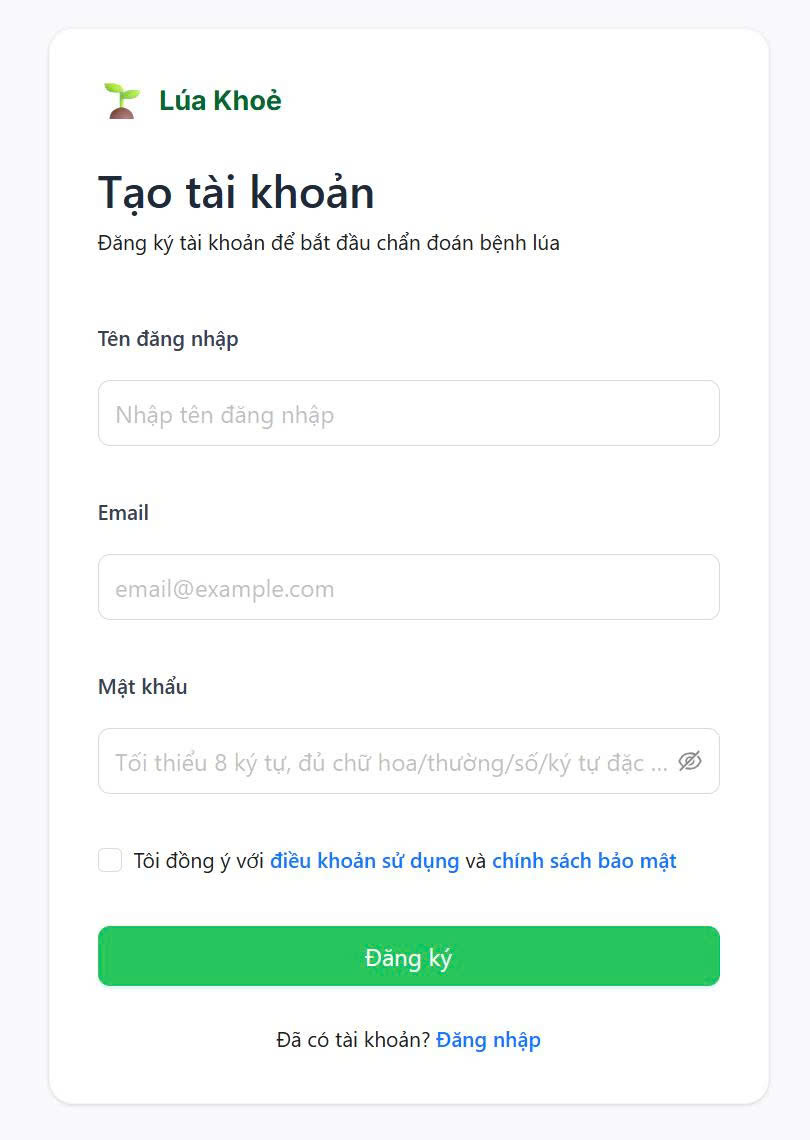
\includegraphics[width=\textwidth,height=0.75\textheight,keepaspectratio]{nd_bm_1.jpg}
    \caption{Giao diện ND\_BM 1: Phiếu đăng ký tài khoản}
    \label{fig:nd-bm-1}
\end{figure}

\vspace{0.3cm}
\noindent\textbf{ND\_BM 1b: ĐĂNG NHẬP HỆ THỐNG}

\begin{figure}[htbp]
    \centering
    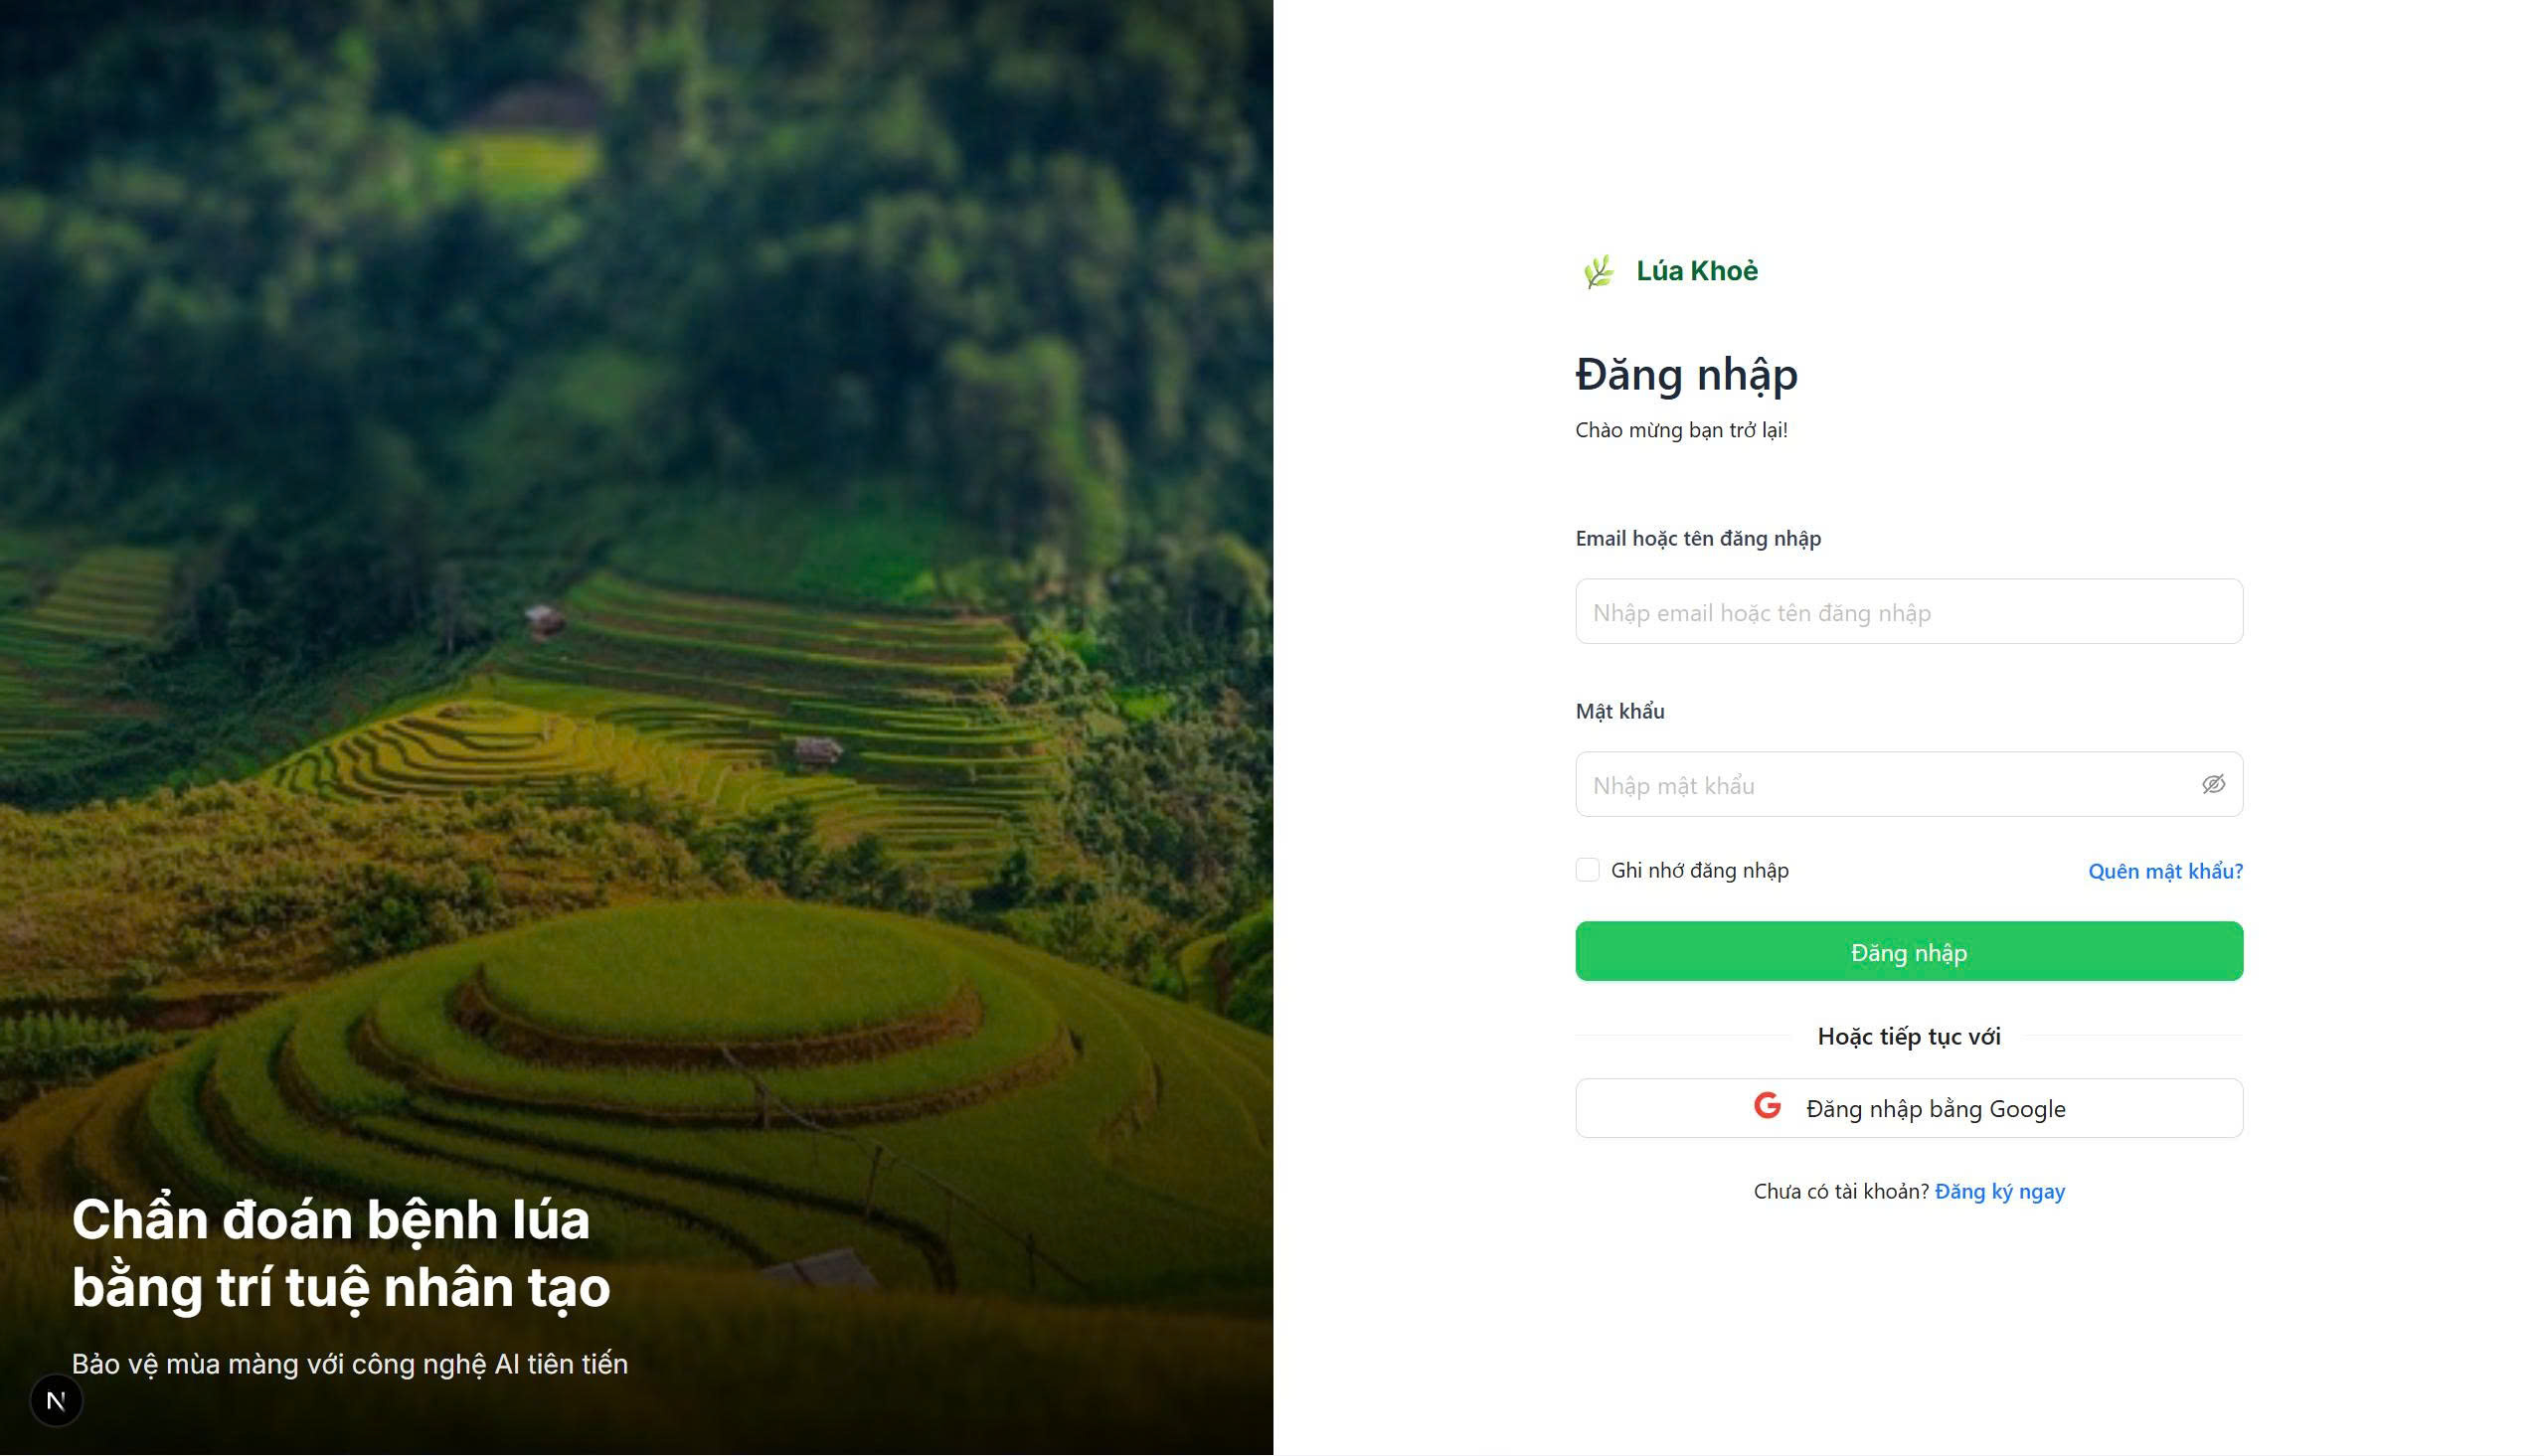
\includegraphics[width=\textwidth,height=0.75\textheight,keepaspectratio]{nd_bm_1b.jpg}
    \caption{Giao diện ND\_BM 1b: Đăng nhập hệ thống}
    \label{fig:nd-bm-1b}
\end{figure}

\vspace{0.3cm}
\noindent\textbf{ND\_BM 1c: ĐỔI MẬT KHẨU}

\begin{figure}[htbp]
    \centering
    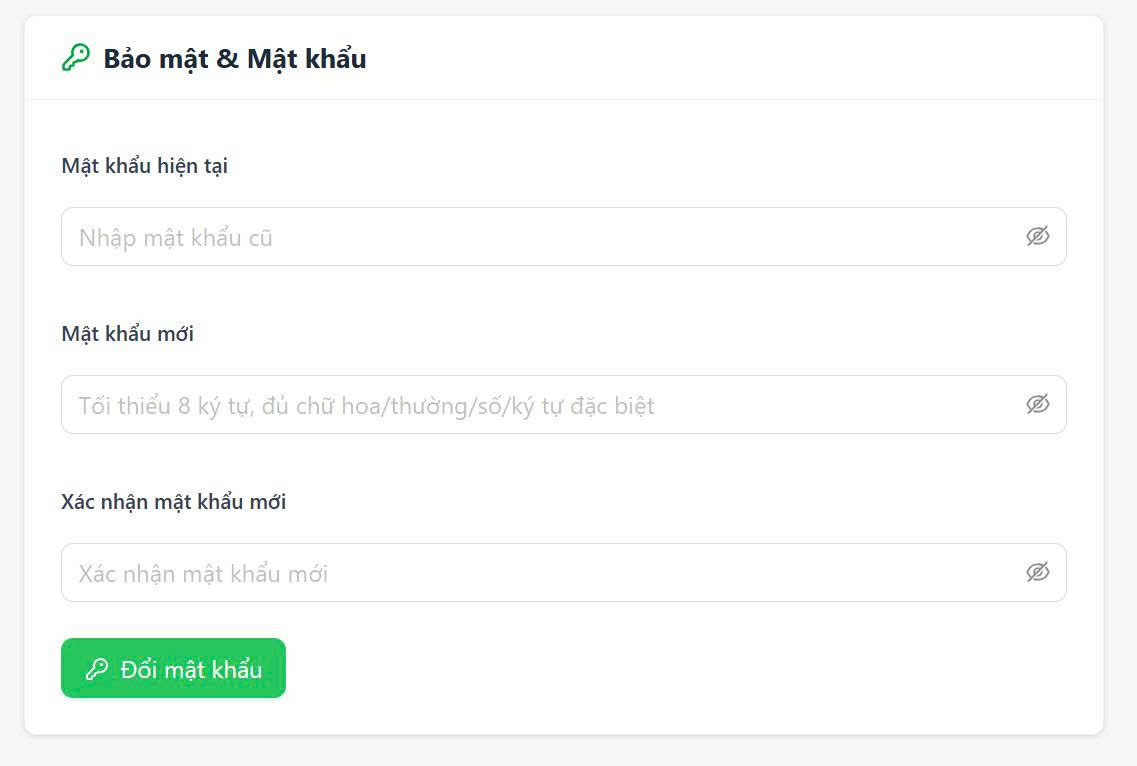
\includegraphics[width=\textwidth,height=0.75\textheight,keepaspectratio]{nd_bm_1c.jpg}
    \caption{Giao diện ND\_BM 1c: Đổi mật khẩu}
    \label{fig:nd-bm-1c}
\end{figure}

\vspace{0.3cm}
\noindent\textbf{ND\_BM 2: PHIẾU CHỈNH SỬA THÔNG TIN CÁ NHÂN}

\begin{figure}[htbp]
    \centering
    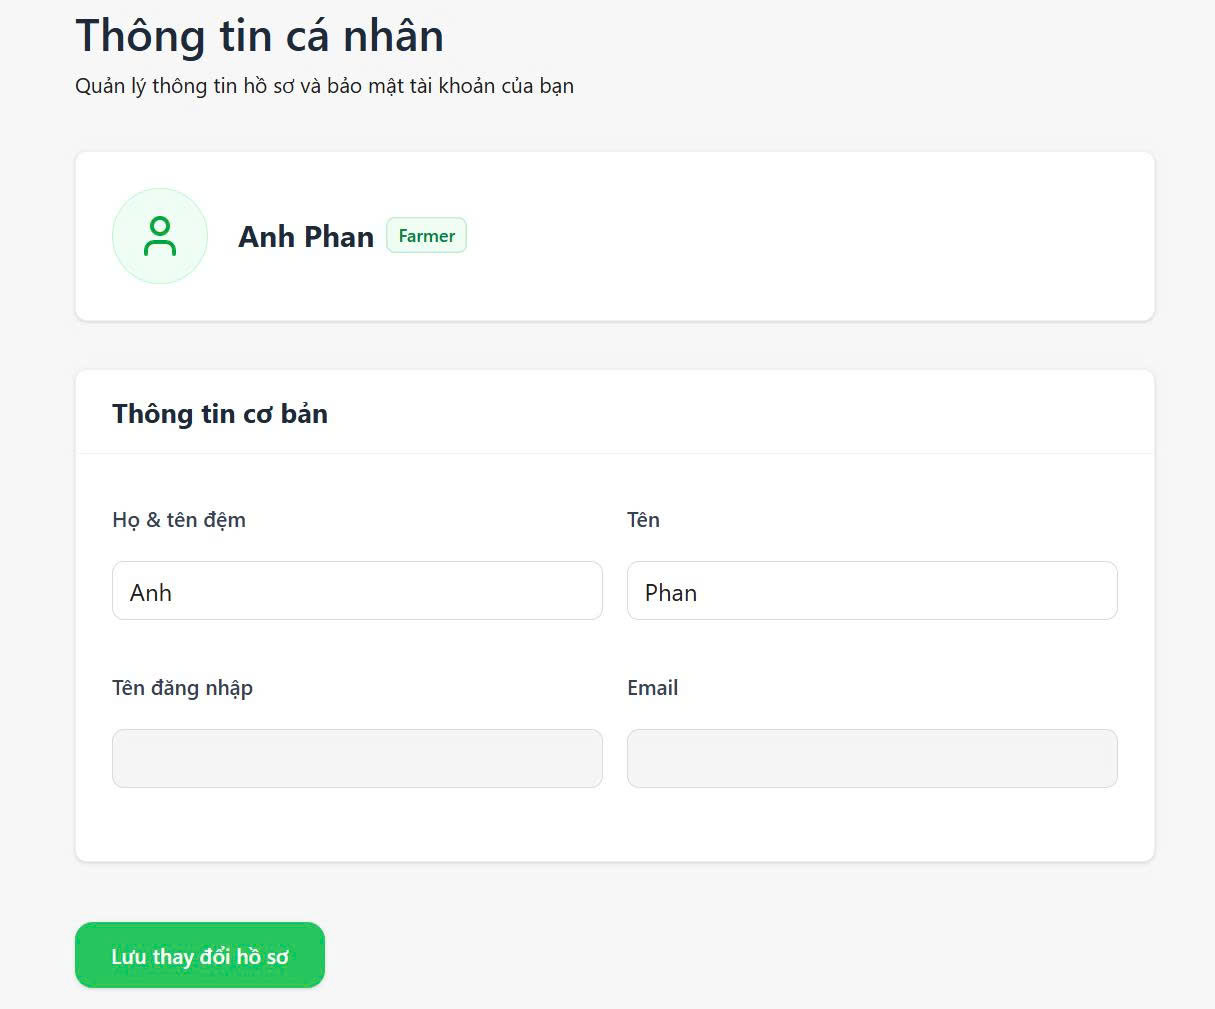
\includegraphics[width=\textwidth,height=0.75\textheight,keepaspectratio]{nd_bm_2.jpg}
    \caption{Giao diện ND\_BM 2: Phiếu chỉnh sửa thông tin cá nhân}
    \label{fig:nd-bm-2}
\end{figure}

\vspace{0.3cm}
\noindent\textbf{ND\_BM 3: PHIẾU GỬI ẢNH CHẨN ĐOÁN}

\begin{figure}[htbp]
    \centering
    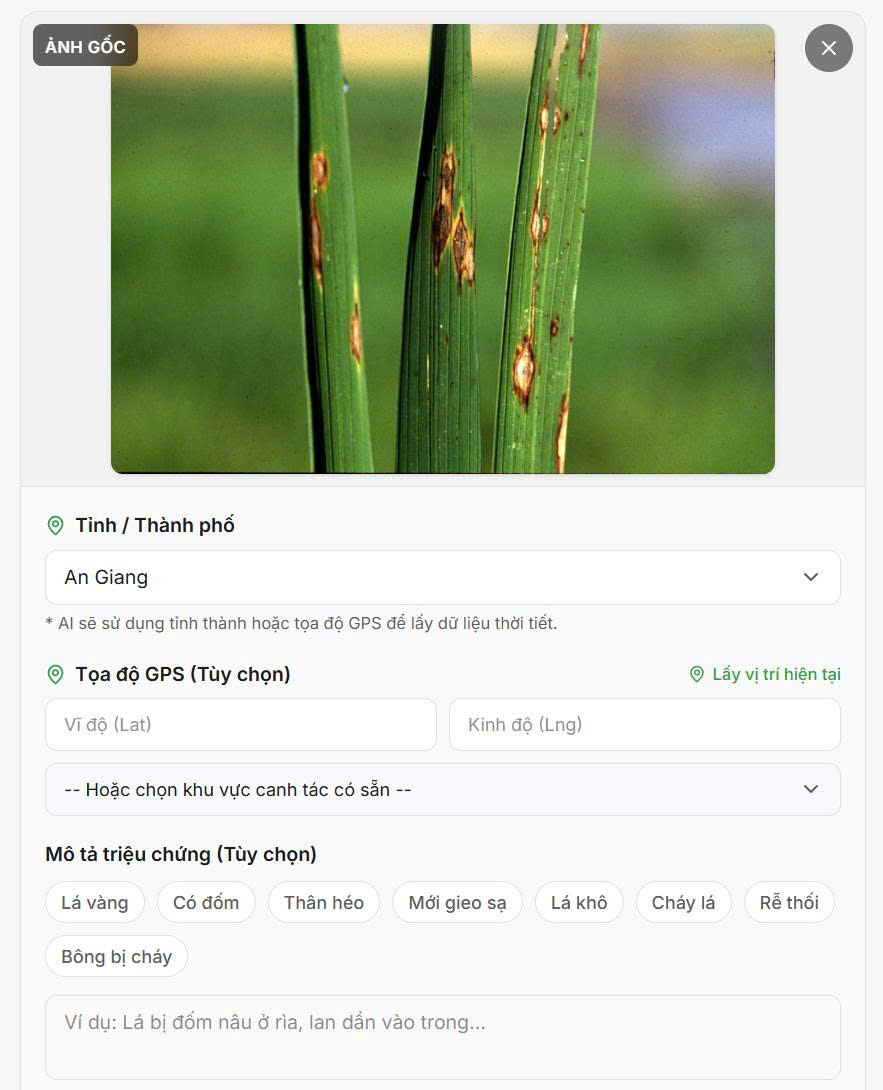
\includegraphics[width=\textwidth,height=0.75\textheight,keepaspectratio]{nd_bm_3.jpg}
    \caption{Giao diện ND\_BM 3: Phiếu gửi ảnh chẩn đoán}
    \label{fig:nd-bm-3}
\end{figure}

\vspace{0.2cm}
\noindent\textbf{ND\_BM 3b: PHIẾU NHẬP THÔNG SỐ MÔI TRƯỜNG} \textit{(tùy chọn)}

\begin{figure}[htbp]
    \centering
    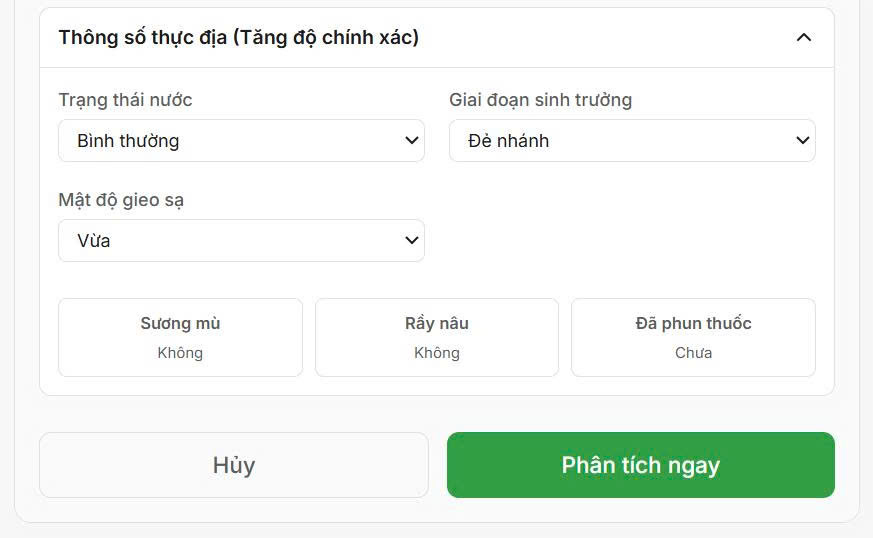
\includegraphics[width=\textwidth,height=0.75\textheight,keepaspectratio]{nd_bm_3b.jpg}
    \caption{Giao diện ND\_BM 3b: Phiếu nhập thông số môi trường (tùy chọn)}
    \label{fig:nd-bm-3b}
\end{figure}

\vspace{0.3cm}
\noindent\textbf{ND\_BM 4: PHIẾU PHẢN HỒI KẾT QUẢ CHẨN ĐOÁN}

\begin{figure}[htbp]
    \centering
    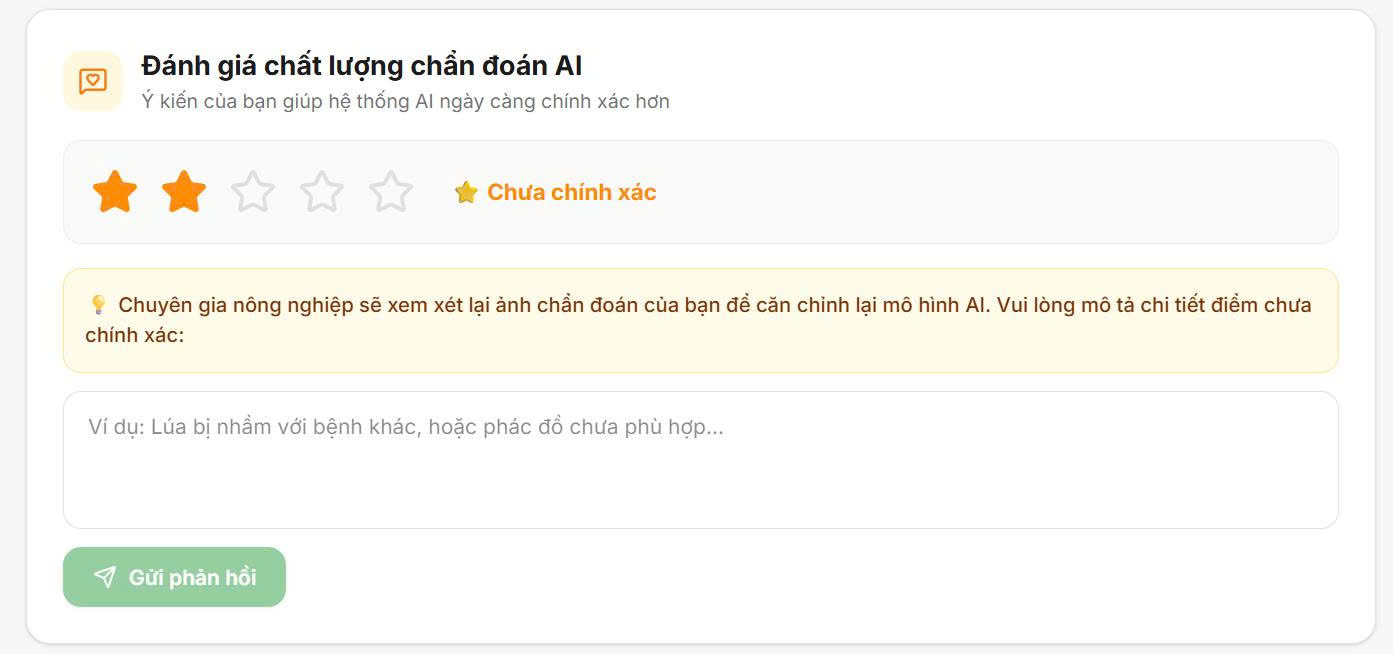
\includegraphics[width=\textwidth,height=0.75\textheight,keepaspectratio]{nd_bm_4.jpg}
    \caption{Giao diện ND\_BM 4: Phiếu phản hồi kết quả chẩn đoán}
    \label{fig:nd-bm-4}
\end{figure}

% ============================================================
% NGƯỜI DÙNG: QUẢN TRỊ VIÊN
% ============================================================
\section{Người dùng --- Quản trị viên (Mã số: AD)}
 
\textbf{Định nghĩa:} Người sử dụng hệ thống với mục đích quản lý danh mục bệnh lúa, kho tri thức dinh dưỡng, tài khoản người dùng và theo dõi hiệu suất mô hình AI.
 
\vspace{0.3cm}
\textbf{1. Bảng yêu cầu chức năng nghiệp vụ}
 
\begin{longtable}{|
        c|
        >{\raggedright\arraybackslash}p{3.2cm}|
        >{\raggedright\arraybackslash}p{2.2cm}|
        >{\raggedright\arraybackslash}p{2.4cm}|
        >{\raggedright\arraybackslash}p{2.6cm}|
        >{\raggedright\arraybackslash}p{2.6cm}|}
    \hline
    \rowcolor{headerblue}
    \textbf{STT} & \textbf{Công việc}               & \textbf{Loại công việc} & \textbf{Quy định/CT liên quan} & \textbf{Biểu mẫu liên quan} & \textbf{Ghi chú} \\
    \hline
    \endhead
    \multicolumn{6}{|l|}{\cellcolor{notegreen}\textbf{I. Tài khoản quản trị}}                                                                                     \\
    \hline
    1            & Đăng nhập hệ thống quản trị      & Tra cứu                 & QĐ-AD-01                       &                             &                  \\
    \hline
    2            & Đổi mật khẩu quản trị            & Lưu trữ                 & QĐ-AD-01                       &                             &                  \\
    \hline
    \multicolumn{6}{|l|}{\cellcolor{notegreen}\textbf{II. Quản lý bệnh lúa}}                                                                                      \\
    \hline
    3            & Xem danh sách bệnh lúa           & Tra cứu                 & QĐ-AD-02                       &                             &                  \\
    \hline
    4            & Thêm bệnh lúa                    & Lưu trữ                 & QĐ-AD-02                       & AD\_BM 1                    &                  \\
    \hline
    5            & Sửa bệnh lúa                     & Lưu trữ                 & QĐ-AD-02                       & AD\_BM 1                    &                  \\
    \hline
    6            & Ẩn / Xóa bệnh lúa                & Lưu trữ                 & QĐ-AD-02                       &                             &                  \\
    \hline
    \multicolumn{6}{|l|}{\cellcolor{notegreen}\textbf{III. Quản lý tri thức dinh dưỡng}}                                                                          \\
    \hline
    7            & Xem danh sách tri thức dinh dưỡng & Tra cứu                & QĐ-AD-03                       &                             &                  \\
    \hline
    8            & Nạp tài liệu dinh dưỡng mới      & Lưu trữ                 & QĐ-AD-03                       & AD\_BM 2                    &                  \\
    \hline
    9            & Xóa phân mảnh tri thức           & Lưu trữ                 & QĐ-AD-03                       &                             &                  \\
    \hline
    \multicolumn{6}{|l|}{\cellcolor{notegreen}\textbf{IV. Quản lý người dùng}}                                                                                    \\
    \hline
    10           & Xem danh sách người dùng         & Tra cứu                 & QĐ-AD-04                       &                             &                  \\
    \hline
    11           & Khóa / Mở khóa tài khoản         & Lưu trữ                 & QĐ-AD-04                       &                             &                  \\
    \hline
    \multicolumn{6}{|l|}{\cellcolor{notegreen}\textbf{V. Quản lý phản hồi}}                                                                                       \\
    \hline
    12           & Xem danh sách phản hồi           & Tra cứu                 & QĐ-AD-05                       &                             &                  \\
    \hline
    13           & Xử lý phản hồi                   & Lưu trữ                 & QĐ-AD-05                       & AD\_BM 3                    &                  \\
    \hline
    \multicolumn{6}{|l|}{\cellcolor{notegreen}\textbf{VI. Hệ thống}}                                                                                              \\
    \hline
    14           & Cập nhật mô hình AI              & Lưu trữ                 & QĐ-AD-06                       &                             &                  \\
    \hline
    15           & Xem thống kê \& báo cáo          & Tra cứu, Kết xuất       & QĐ-AD-06                       & AD\_BM 4                    &                  \\
    \hline
\end{longtable}
 
% ============================================================
\vspace{0.3cm}
\textbf{2. Bảng Quy định / Công thức liên quan --- Quản trị viên}
 
\begin{longtable}{|
        c|
        >{\raggedright\arraybackslash}p{1.8cm}|
        >{\raggedright\arraybackslash}p{3.4cm}|
        >{\raggedright\arraybackslash}p{6.4cm}|
        >{\raggedright\arraybackslash}p{1.4cm}|}
    \hline
    \rowcolor{headerblue}
    \textbf{STT} & \textbf{Mã số} & \textbf{Tên Quy định}                & \textbf{Mô tả chi tiết}                                                                                                                         & \textbf{Ghi chú} \\
    \hline
    \endhead
    1            & QĐ-AD-01       & Quy định Tài khoản quản trị          & Bao gồm quy trình đăng nhập (kiểm tra tên đăng nhập + mật khẩu, khóa sau 5 lần sai trong 30 phút) và đổi mật khẩu.                              &                  \\
    \hline
    2            & QĐ-AD-02       & Quy định Quản lý bệnh lúa            & Bao gồm quy trình thêm, sửa, ẩn/xóa bệnh lúa. Upload ảnh riêng trước khi lưu. Ràng buộc severity, imageUrl, treatment. Chỉ ADMIN được thay đổi. &                  \\
    \hline
    3            & QĐ-AD-03       & Quy định Quản lý tri thức dinh dưỡng & Bao gồm quy trình nạp tài liệu 4 bước và xóa theo chunk ID. Ràng buộc vector 3072 chiều, bảo toàn phân số, giới hạn RAG context window.          &                  \\
    \hline
    4            & QĐ-AD-04       & Quy định Quản lý người dùng          & Bao gồm quy trình xem danh sách và khóa/mở khóa tài khoản. Quản trị viên không được chỉnh sửa thông tin cá nhân của người dùng.                 &                  \\
    \hline
    5            & QĐ-AD-05       & Quy định Xử lý phản hồi              & Bao gồm quy trình xem danh sách phiếu phản hồi, xem xét kết quả và chốt trạng thái xử lý.                                                      &                  \\
    \hline
    6            & QĐ-AD-06       & Quy định Hệ thống                    & Bao gồm quy trình cập nhật mô hình AI và xem thống kê/báo cáo hiệu suất.                                                                       &                  \\
    \hline
\end{longtable}
 
% ============================================================
\vspace{0.3cm}
\textbf{3. Chi tiết từng Quy định --- Quản trị viên}
 
% ---- QĐ-AD-01 ----
\vspace{0.3cm}
\noindent\textbf{QĐ-AD-01 --- Quy định Tài khoản quản trị}
 
\begin{longtable}{|
    >{\raggedright\arraybackslash}p{2.8cm}|
    >{\raggedright\arraybackslash}p{12cm}|}
\hline
\rowcolor{headerblue}
\textbf{Chức năng} & \textbf{Quy trình \& Ràng buộc} \\
\hline
\endhead
\textbf{a) Đăng nhập hệ thống quản trị} &
Quản trị viên phải nhập đầy đủ 2 thông tin sau (không được để trống):
\begin{itemize}[leftmargin=*,topsep=2pt,itemsep=1pt]
    \item \textbf{Tên đăng nhập:} phải tồn tại trong hệ thống.
    \item \textbf{Mật khẩu:} phải khớp với tài khoản tương ứng.
\end{itemize}
\textbf{Cơ chế bảo mật:} Nếu đăng nhập sai, hệ thống chỉ hiển thị thông báo chung ``Tên đăng nhập hoặc mật khẩu không chính xác'' mà không chỉ rõ trường nào sai. Nhập sai 5 lần liên tiếp thì khóa tài khoản 30 phút. \\
\textbf{Quy tắc xử lý:} Đăng nhập thành công thì chuyển vào trang quản trị. \\
\hline
\textbf{b) Đổi mật khẩu} &
Quản trị viên thực hiện theo các bước sau:
\begin{enumerate}[leftmargin=*,topsep=2pt,itemsep=1pt]
    \item Nhập \textbf{mật khẩu hiện tại} để hệ thống xác thực.
    \item Nhập \textbf{mật khẩu mới} --- phải đáp ứng độ mạnh (tối thiểu 8 ký tự, gồm chữ hoa, chữ số và ký tự đặc biệt) và không được trùng mật khẩu cũ.
    \item Nhập \textbf{xác nhận mật khẩu mới} --- phải gõ chính xác giống bước 2.
\end{enumerate}
\textbf{Quy tắc xử lý:} Hệ thống cập nhật mật khẩu mới và tự động hủy các phiên đăng nhập đang tồn tại trên các thiết bị khác. \\
\hline
\end{longtable}
 
% ---- QĐ-AD-02 ----
\vspace{0.3cm}
\noindent\textbf{QĐ-AD-02 --- Quy định Quản lý bệnh lúa}
 
\begin{longtable}{|
    >{\raggedright\arraybackslash}p{2.8cm}|
    >{\raggedright\arraybackslash}p{12cm}|}
\hline
\rowcolor{headerblue}
\textbf{Chức năng} & \textbf{Quy trình \& Ràng buộc} \\
\hline
\endhead
\textbf{a) Xem danh sách bệnh lúa} &
Hệ thống hiển thị toàn bộ danh sách bệnh lúa hiện có, bao gồm cả các bệnh đang ở trạng thái ``Ẩn''. Quản trị viên có thể lọc và tìm kiếm theo tên bệnh. \\
\hline
\textbf{b) Thêm bệnh lúa} &
Thực hiện theo 2 bước:
\begin{enumerate}[leftmargin=*,topsep=2pt,itemsep=1pt]
    \item \textbf{Upload ảnh minh họa (nếu có):} Quản trị viên chọn file ảnh, hệ thống gửi lên Cloudinary qua API độc lập và trả về đường dẫn ảnh (\texttt{secure\_url}).
    \item \textbf{Điền thông tin và lưu:} Quản trị viên nhập đầy đủ thông tin bệnh (bao gồm đường dẫn ảnh từ bước 1 nếu có) rồi gửi lên hệ thống.
\end{enumerate}
\textbf{Ràng buộc dữ liệu:}
\begin{itemize}[leftmargin=*,topsep=2pt,itemsep=1pt]
    \item \textbf{Tên bệnh và tên khoa học:} phải là duy nhất trong hệ thống.
    \item \textbf{Mức độ nghiêm trọng (severity):} chỉ nhận 1 trong 3 giá trị \texttt{low / medium / high}, mặc định là \texttt{medium}.
    \item \textbf{Đường dẫn ảnh (imageUrl):} tối đa 512 ký tự, có thể để trống nếu chưa có ảnh.
    \item \textbf{Phác đồ điều trị (treatment):} kiểu văn bản dài, không giới hạn số ký tự.
\end{itemize}
\textbf{Phân quyền:} Chỉ tài khoản có quyền ADMIN mới được thực hiện thao tác này. \\
\hline
\textbf{c) Sửa bệnh lúa} &
Quản trị viên có thể chỉnh sửa toàn bộ thông tin của bản ghi bệnh (tên, mức độ, triệu chứng, phác đồ, ảnh). Nếu muốn đổi ảnh, cần upload ảnh mới trước để lấy đường dẫn mới. \\
\textbf{Ràng buộc:} Không được thay đổi mã định danh hệ thống (ID) của bản ghi. \\
\textbf{Phân quyền:} Chỉ tài khoản có quyền ADMIN mới được thực hiện thao tác này. \\
\hline
\textbf{d) Ẩn / Xóa bệnh lúa} &
Hệ thống áp dụng 2 cơ chế tùy theo tình trạng dữ liệu:
\begin{itemize}[leftmargin=*,topsep=2pt,itemsep=1pt]
    \item \textbf{Xóa vĩnh viễn:} chỉ áp dụng khi bệnh chưa có bất kỳ dữ liệu lịch sử chẩn đoán nào liên quan.
    \item \textbf{Chuyển sang trạng thái ``Ẩn'':} áp dụng khi bệnh đã có lịch sử chẩn đoán --- dữ liệu cũ được bảo toàn nguyên vẹn, không bị xóa theo.
\end{itemize}
\textbf{Phân quyền:} Chỉ tài khoản có quyền ADMIN mới được thực hiện thao tác này. \\
\hline
\end{longtable}
 
% ---- QĐ-AD-03 ----
\vspace{0.3cm}
\noindent\textbf{QĐ-AD-03 --- Quy định Quản lý tri thức dinh dưỡng}
 
\begin{longtable}{|
    >{\raggedright\arraybackslash}p{2.8cm}|
    >{\raggedright\arraybackslash}p{12cm}|}
\hline
\rowcolor{headerblue}
\textbf{Chức năng} & \textbf{Quy trình \& Ràng buộc} \\
\hline
\endhead
\textbf{a) Xem danh sách tri thức dinh dưỡng} &
Hệ thống hiển thị danh sách các phân mảnh tri thức (chunk) hiện có trong kho, bao gồm nội dung, nguồn tài liệu và siêu dữ liệu liên quan. \\
\hline
\textbf{b) Nạp tài liệu dinh dưỡng mới} &
Thực hiện theo 4 bước tuần tự:
\begin{enumerate}[leftmargin=*,topsep=2pt,itemsep=1pt]
    \item \textbf{Đọc file:} Với file \texttt{.txt} và \texttt{.md}, trình duyệt đọc trực tiếp bằng \texttt{FileReader.readAsText()} mà không cần gửi lên server. Với file \texttt{.pdf}, file được đẩy lên backend để bóc tách nội dung.
    \item \textbf{Lọc rác:} Nội dung thô đi qua hàm \texttt{cleanPDFText()} để loại bỏ ký tự rác, số trang cô lập và hàn gắn các dòng bị bẻ gãy. \textbf{Lưu ý quan trọng:} bộ lọc phải bảo toàn nguyên vẹn các tỷ lệ hóa chất nông nghiệp (ví dụ: ``bón 1/2 liều lượng'', ``pha tỷ lệ 1/3'').
    \item \textbf{Băm nhỏ:} Văn bản sạch được băm thành các phân mảnh (chunk) dựa trên ranh giới tiêu đề Markdown (\#, \#\#, \#\#\#) qua hàm \texttt{splitMarkdown()}.
    \item \textbf{Vector hóa và lưu trữ:} Từng chunk được gửi tới API nhúng của Google (\texttt{GoogleGenerativeAIEmbeddings}) để tạo vector \textbf{3072 chiều}. Nội dung, siêu dữ liệu và vector được lưu vào bảng \texttt{nutritions}.
\end{enumerate}
\textbf{Ràng buộc kỹ thuật:}
\begin{itemize}[leftmargin=*,topsep=2pt,itemsep=1pt]
    \item Vector bắt buộc phải có đúng \textbf{3072 chiều} --- sai số chiều thì cơ sở dữ liệu từ chối ngay lập tức.
    \item Mỗi lần truy vấn RAG chỉ được lấy tối đa số chunk theo cấu hình \texttt{RAG\_CONTEXT\_WINDOW} (mặc định 3--5 chunk/bệnh) để tránh tràn bộ nhớ token của mô hình ngôn ngữ.
    \item Khi phát hiện nhiều bệnh cùng lúc, hệ thống tìm kiếm đa luồng và loại bỏ các chunk trùng lặp trước khi đưa vào mô hình ngôn ngữ.
\end{itemize}
\textbf{Phân quyền:} Chỉ tài khoản có quyền ADMIN mới được nạp tài liệu mới. \\
\hline
\textbf{c) Xóa phân mảnh tri thức} &
Quản trị viên xóa từng phân mảnh tri thức theo ID (UUID). Hệ thống giải phóng không gian lưu trữ vector trong cơ sở dữ liệu. \\
\textbf{Phân quyền:} Chỉ tài khoản có quyền ADMIN mới được thực hiện thao tác này. \\
\hline
\end{longtable}
 
% ---- QĐ-AD-04 ----
\vspace{0.3cm}
\noindent\textbf{QĐ-AD-04 --- Quy định Quản lý người dùng}
 
\begin{longtable}{|
    >{\raggedright\arraybackslash}p{2.8cm}|
    >{\raggedright\arraybackslash}p{12cm}|}
\hline
\rowcolor{headerblue}
\textbf{Chức năng} & \textbf{Quy trình \& Ràng buộc} \\
\hline
\endhead
\textbf{a) Xem danh sách người dùng} &
Hệ thống hiển thị danh sách người dùng với các thông tin: tên đăng nhập, email, số lượt chẩn đoán, số lượt phản hồi và trạng thái tài khoản. \\
\hline
\textbf{b) Khóa / Mở khóa tài khoản} &
Quản trị viên thực hiện theo các bước sau:
\begin{enumerate}[leftmargin=*,topsep=2pt,itemsep=1pt]
    \item Chọn tài khoản cần thay đổi trạng thái.
    \item Chuyển trạng thái giữa ``Hoạt động'' và ``Tạm khóa''.
\end{enumerate}
\textbf{Ràng buộc:} Quản trị viên không được chỉnh sửa tên đăng nhập, email hoặc bất kỳ thông tin cá nhân nào của người dùng. \\
\hline
\end{longtable}
 
% ---- QĐ-AD-05 ----
\vspace{0.3cm}
\noindent\textbf{QĐ-AD-05 --- Quy định Xử lý phản hồi}
 
\begin{longtable}{|
    >{\raggedright\arraybackslash}p{2.8cm}|
    >{\raggedright\arraybackslash}p{12cm}|}
\hline
\rowcolor{headerblue}
\textbf{Chức năng} & \textbf{Quy trình \& Ràng buộc} \\
\hline
\endhead
\textbf{a) Xem danh sách phản hồi} &
Hệ thống hiển thị danh sách phiếu phản hồi chưa xử lý, ưu tiên phiếu gửi sớm nhất. \\
\hline
\textbf{b) Xử lý phản hồi} &
Quản trị viên thực hiện theo 4 bước tuần tự:
\begin{enumerate}[leftmargin=*,topsep=2pt,itemsep=1pt]
    \item Xem danh sách phiếu chưa xử lý, ưu tiên phiếu gửi sớm nhất.
    \item Xem xét song song: ảnh gốc, kết quả AI và kết quả nông dân báo cáo.
    \item Nhập lời nhắn phản hồi gửi lại cho nông dân.
    \item Chốt trạng thái xử lý: ``Chấp nhận'' (AI sai) hoặc ``Từ chối'' (AI đúng).
\end{enumerate}
\textbf{Quy tắc xử lý:} Nếu chọn ``Chấp nhận'', hệ thống tự động lưu ảnh vào tập dữ liệu để nâng cấp mô hình AI sau này. \\
\hline
\end{longtable}
 
% ---- QĐ-AD-06 ----
\vspace{0.3cm}
\noindent\textbf{QĐ-AD-06 --- Quy định Hệ thống}
 
\begin{longtable}{|
    >{\raggedright\arraybackslash}p{2.8cm}|
    >{\raggedright\arraybackslash}p{12cm}|}
\hline
\rowcolor{headerblue}
\textbf{Chức năng} & \textbf{Quy trình \& Ràng buộc} \\
\hline
\endhead
\textbf{a) Cập nhật mô hình AI} &
Quản trị viên thực hiện theo các bước sau:
\begin{enumerate}[leftmargin=*,topsep=2pt,itemsep=1pt]
    \item Tải lên file mô hình AI mới kèm tên phiên bản và ghi chú thay đổi.
    \item Hệ thống lưu file mô hình ở trạng thái chưa kích hoạt.
    \item Quản trị viên dùng công tắc ``Kích hoạt'' để áp dụng mô hình mới cho toàn hệ thống. Mô hình cũ tự động tắt.
\end{enumerate} \\
\hline
\textbf{b) Xem thống kê \& báo cáo} &
Hệ thống hiển thị 2 loại báo cáo:
\begin{itemize}[leftmargin=*,topsep=2pt,itemsep=1pt]
    \item \textbf{Bản đồ dịch bệnh:} bản đồ nhiệt tình hình dịch bệnh theo tọa độ GPS của các ca chẩn đoán.
    \item \textbf{Hiệu suất AI:} thống kê tỷ lệ chẩn đoán đúng/sai theo từng loại bệnh dựa trên kết quả xử lý phản hồi.
\end{itemize} \\
\hline
\end{longtable}
 
% ============================================================
\vspace{0.3cm}
\textbf{4. Các Biểu mẫu --- Quản trị viên}
 
\vspace{0.3cm}
\noindent\textbf{AD\_BM 1: PHIẾU QUẢN LÝ BỆNH LÚA}
 
\begin{figure}[H]
    \centering
    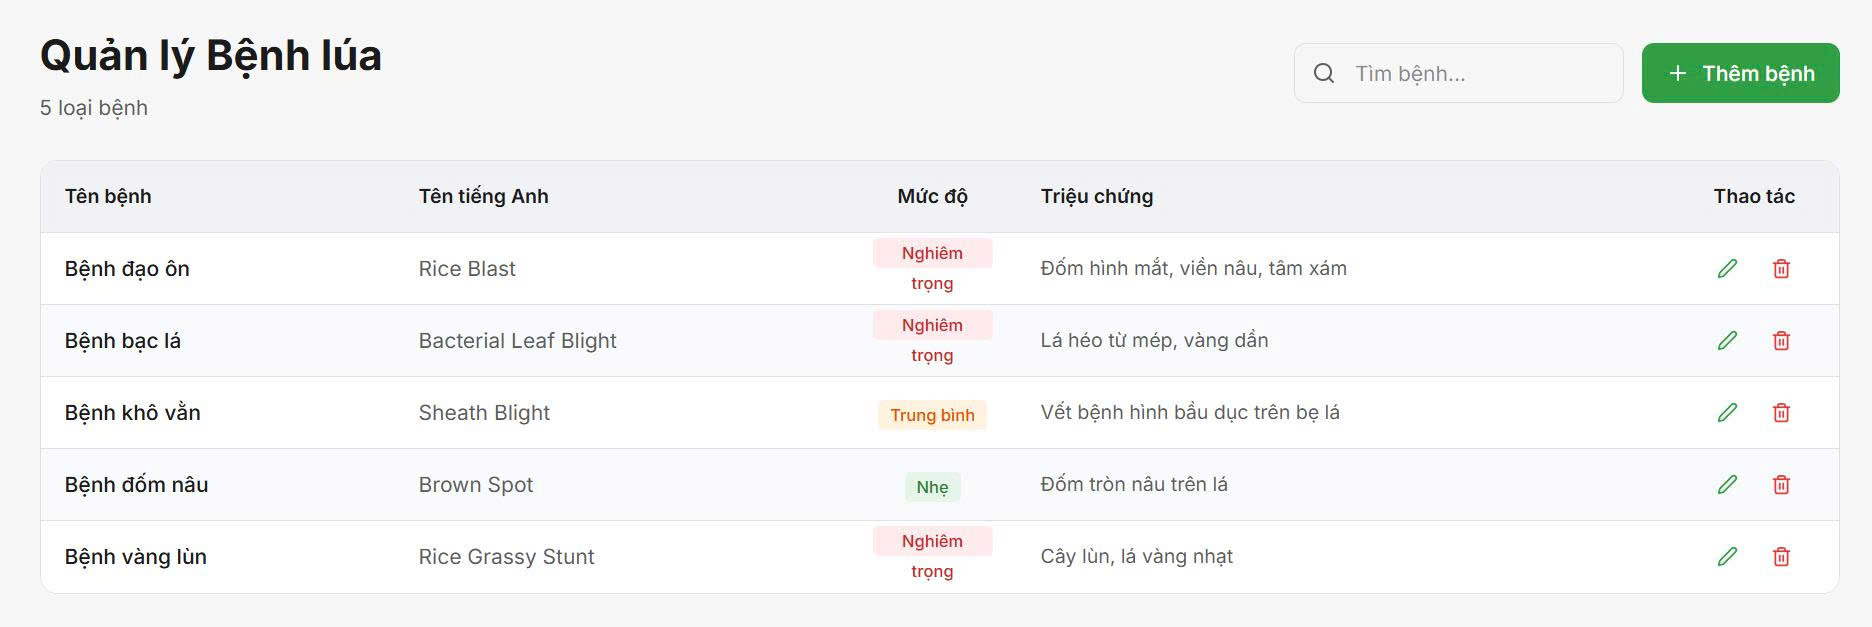
\includegraphics[width=\textwidth,height=0.75\textheight,keepaspectratio]{ad_bm_1.jpg}
    \caption{Giao diện AD\_BM 1: Phiếu quản lý bệnh lúa}
    \label{fig:ad-bm-1}
\end{figure}
 
\vspace{0.3cm}
\noindent\textbf{AD\_BM 2: PHIẾU QUẢN LÝ TRI THỨC DINH DƯỠNG}
 
\begin{figure}[H]
    \centering
    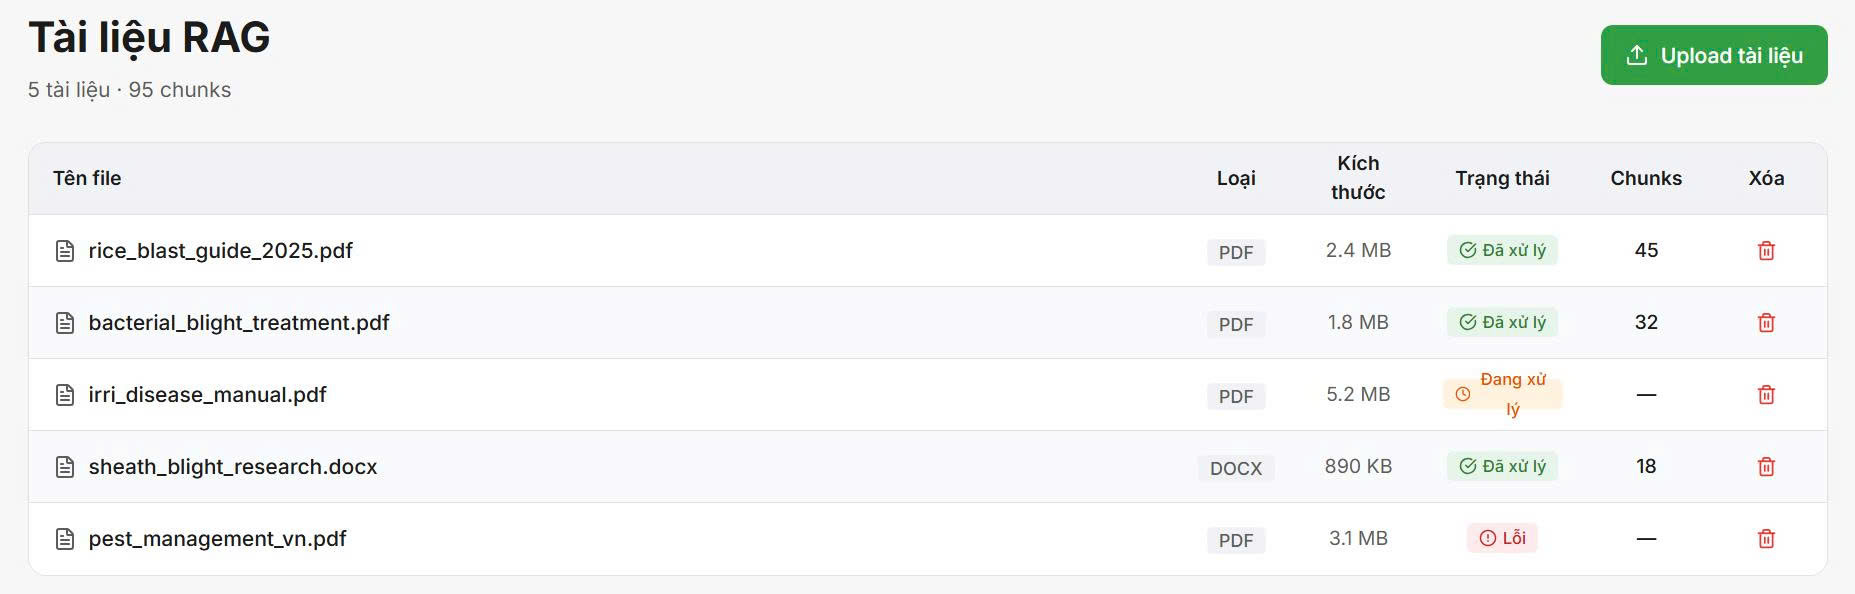
\includegraphics[width=\textwidth,height=0.75\textheight,keepaspectratio]{ad_bm_2.jpg}
    \caption{Giao diện AD\_BM 2: Phiếu quản lý tri thức dinh dưỡng}
    \label{fig:ad-bm-2}
\end{figure}
 
\vspace{0.3cm}
\noindent\textbf{AD\_BM 3: PHIẾU XỬ LÝ PHẢN HỒI}
 
\begin{figure}[H]
    \centering
    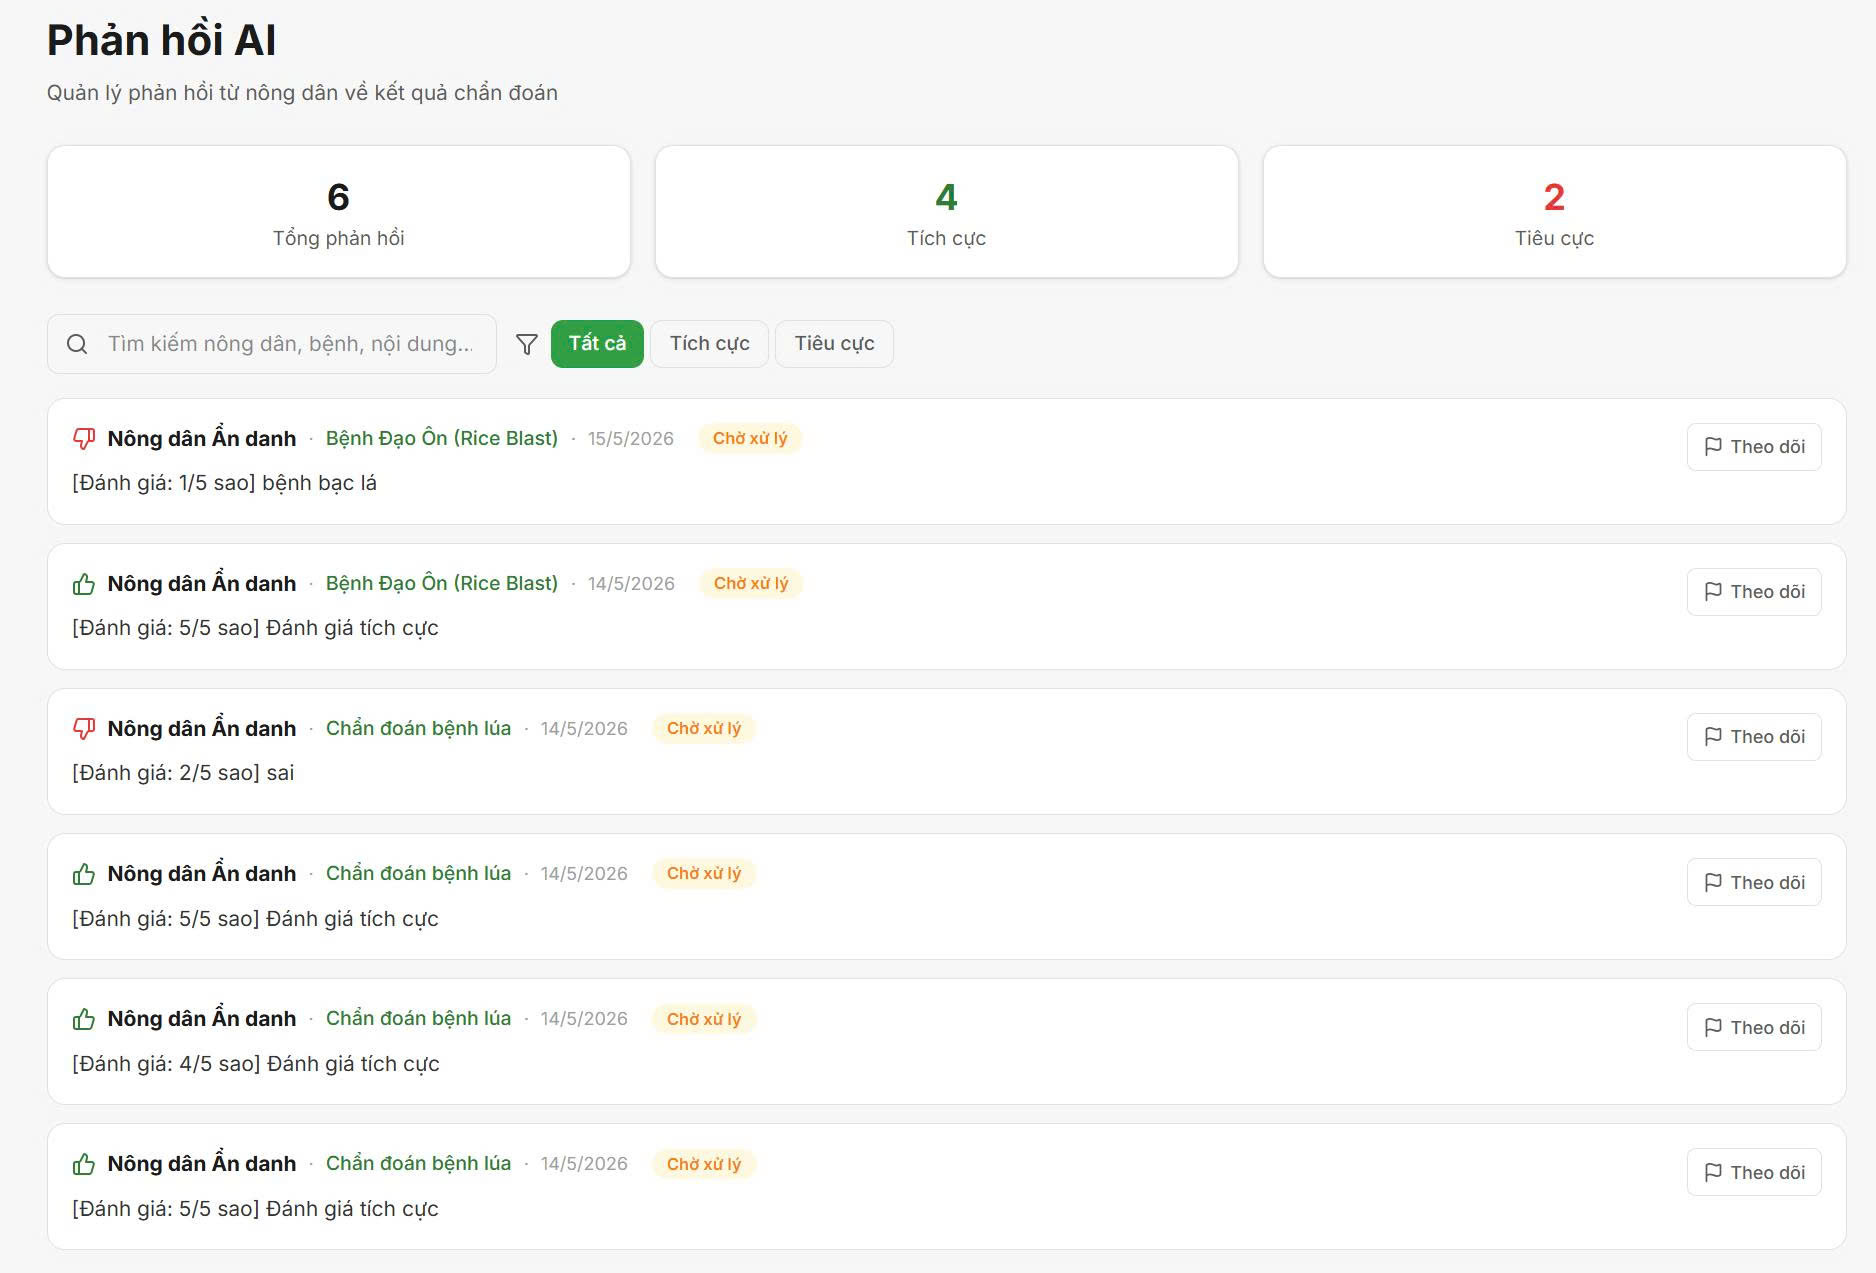
\includegraphics[width=\textwidth,height=0.75\textheight,keepaspectratio]{ad_bm_3.jpg}
    \caption{Giao diện AD\_BM 3: Phiếu xử lý phản hồi}
    \label{fig:ad-bm-3}
\end{figure}
 
\vspace{0.3cm}
\noindent\textbf{AD\_BM 4: BÁO CÁO HIỆU SUẤT AI}
 
\begin{figure}[H]
    \centering
    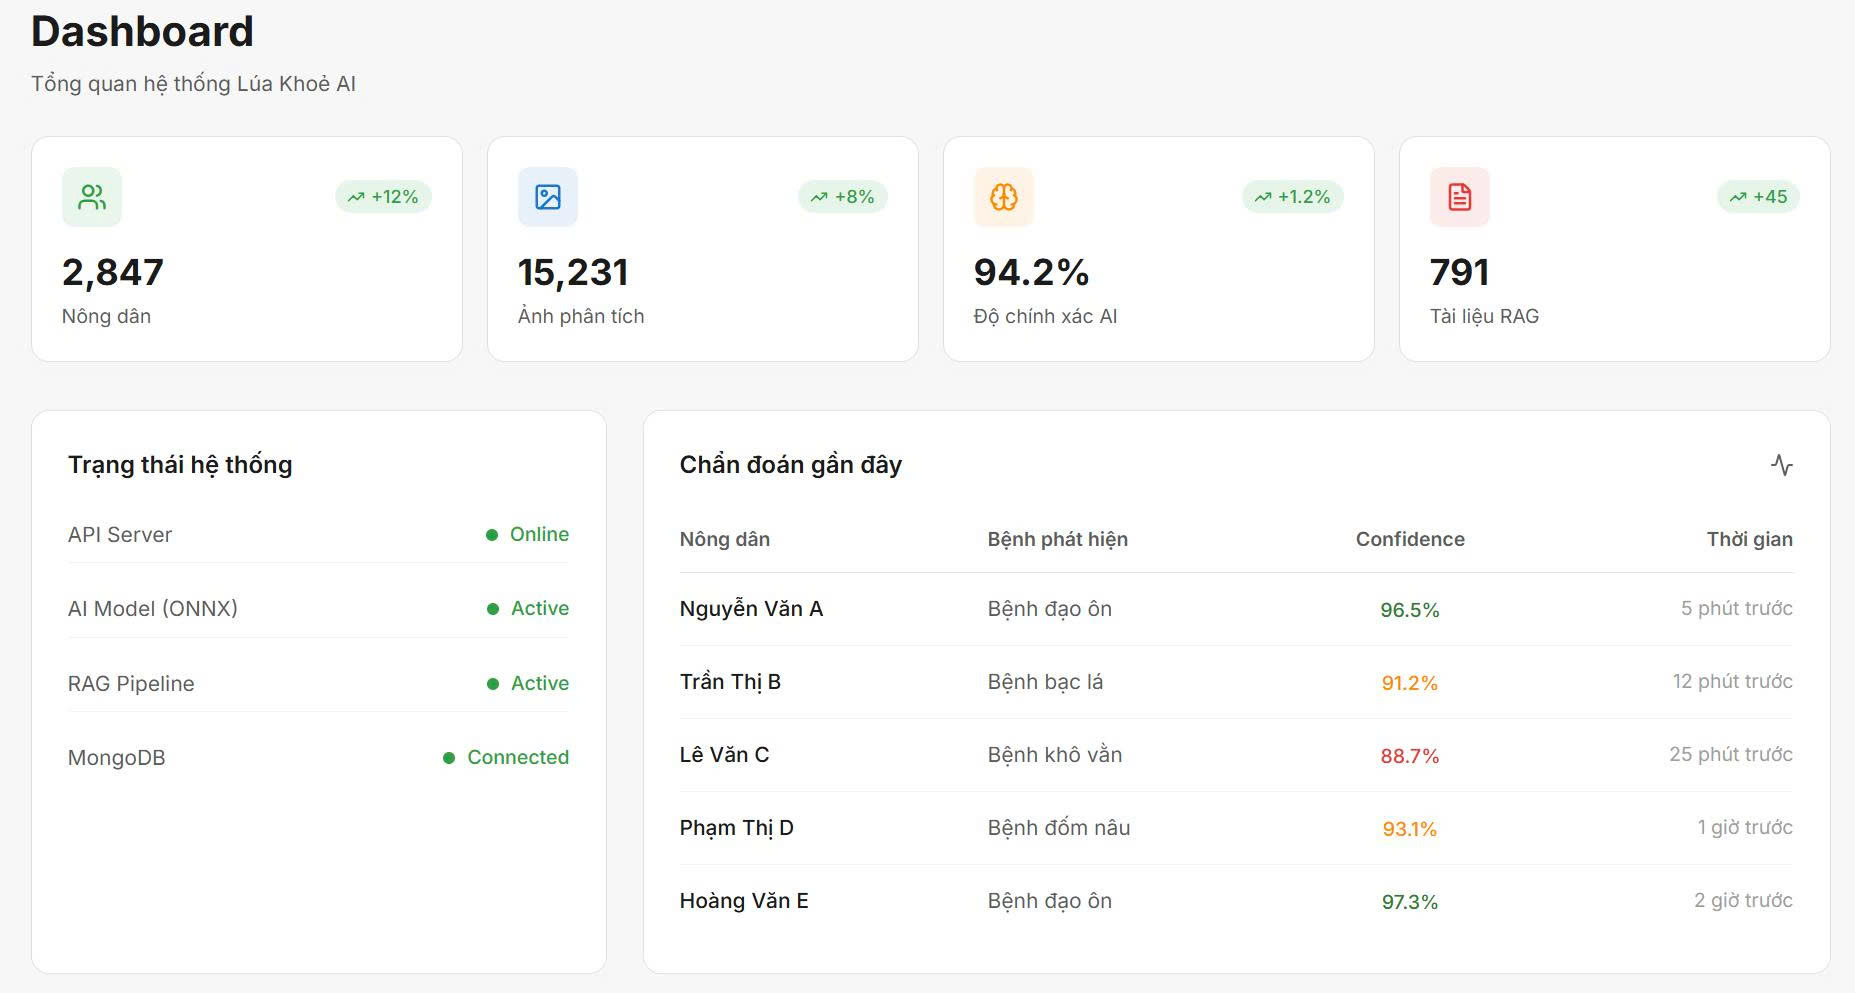
\includegraphics[width=\textwidth,height=0.75\textheight,keepaspectratio]{ad_bm_4.jpg}
    \caption{Giao diện AD\_BM 4: Báo cáo hiệu suất AI}
    \label{fig:ad-bm-4}
\end{figure}

% ============================================================
\vspace{0.3cm}
\textbf{4. Các Biểu mẫu --- Quản trị viên}

\vspace{0.3cm}
\noindent\textbf{AD\_BM 1: PHIẾU QUẢN LÝ BỆNH LÚA}

\begin{figure}[H]
    \centering
    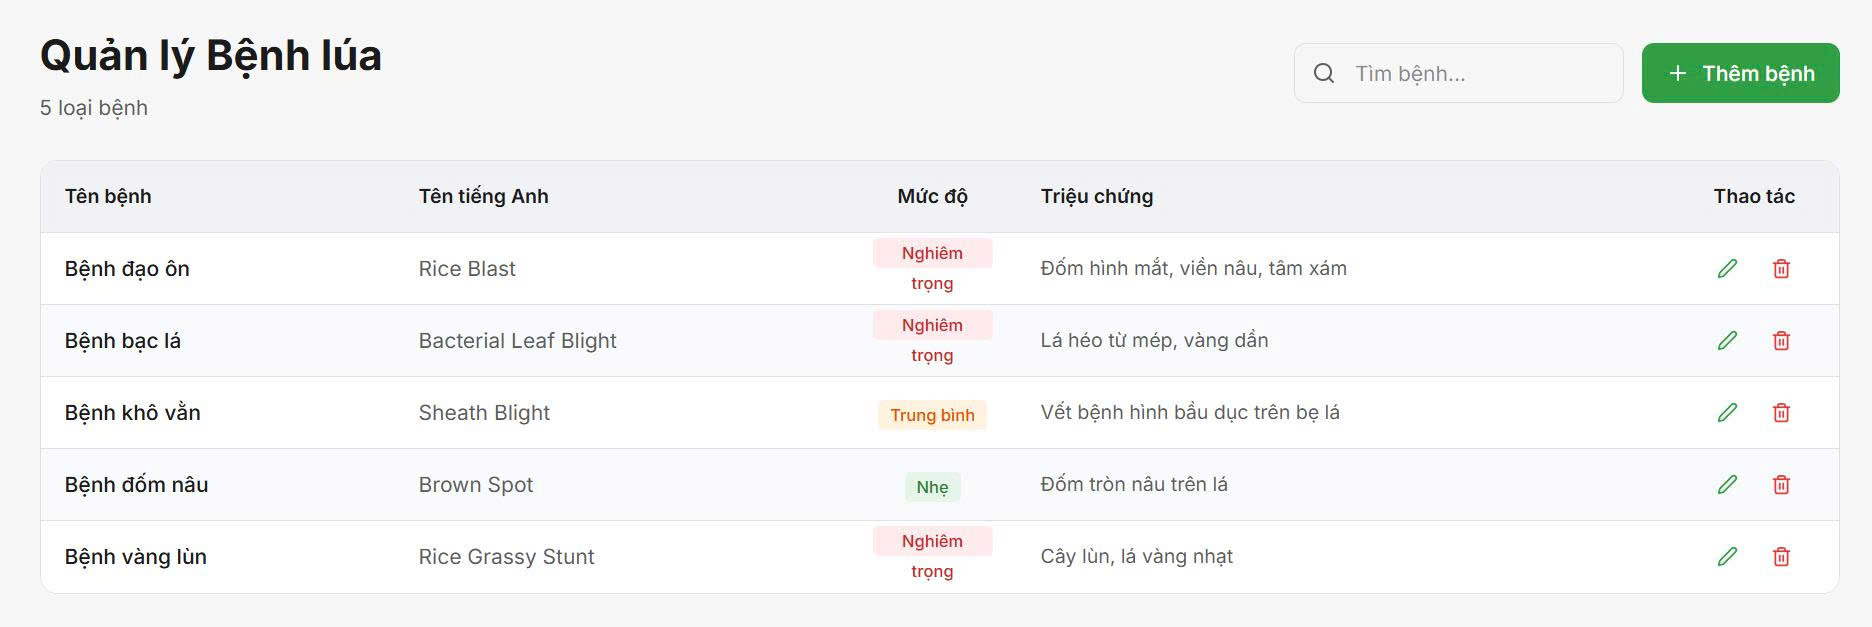
\includegraphics[width=\textwidth,height=0.75\textheight,keepaspectratio]{ad_bm_1.jpg}
    \caption{Giao diện AD\_BM 1: Phiếu quản lý bệnh lúa}
    \label{fig:ad-bm-1}
\end{figure}

\vspace{0.3cm}
\noindent\textbf{AD\_BM 2: PHIẾU QUẢN LÝ TRI THỨC DINH DƯỠNG}

\begin{figure}[H]
    \centering
    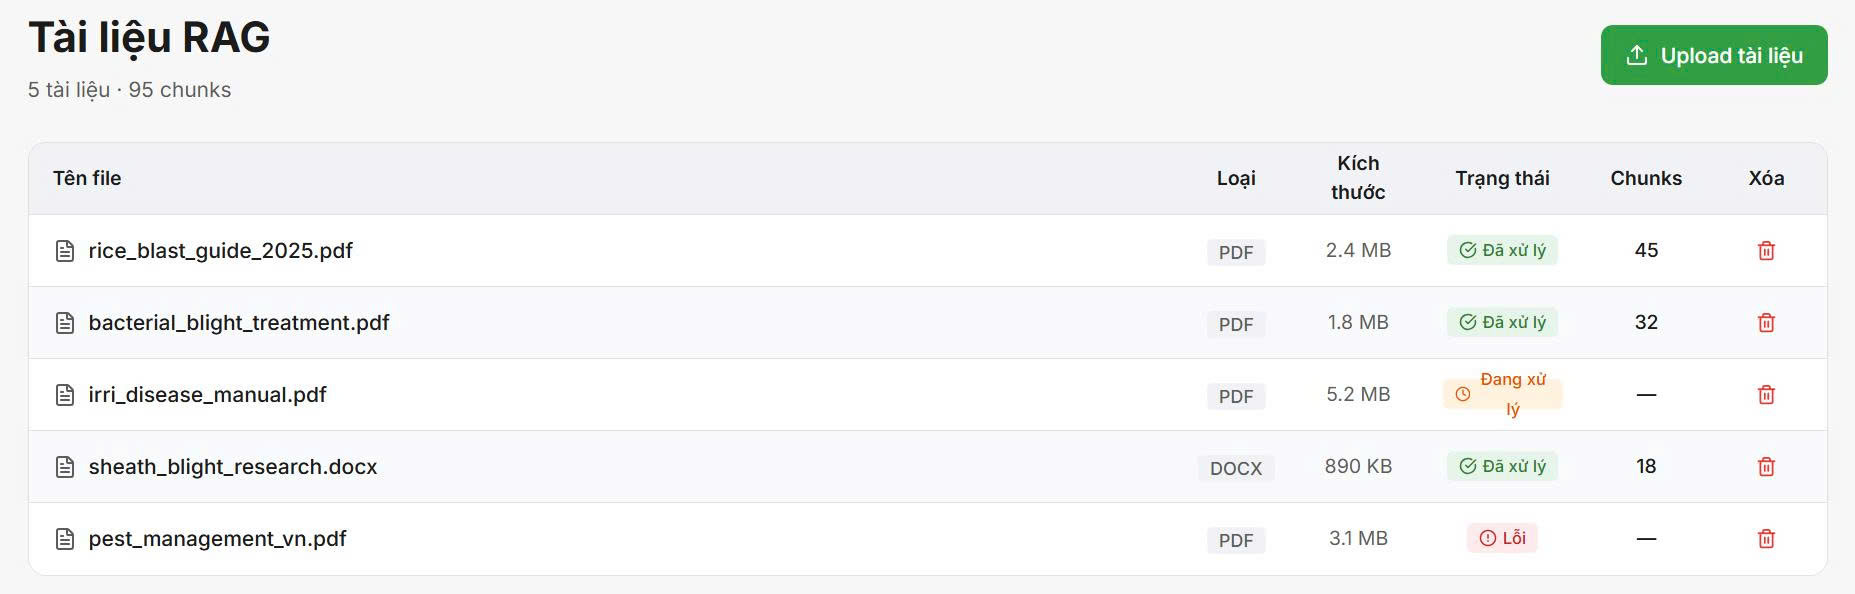
\includegraphics[width=\textwidth,height=0.75\textheight,keepaspectratio]{ad_bm_2.jpg}
    \caption{Giao diện AD\_BM 2: Phiếu quản lý tri thức dinh dưỡng}
    \label{fig:ad-bm-2}
\end{figure}

\vspace{0.3cm}
\noindent\textbf{AD\_BM 3: PHIẾU XỬ LÝ PHẢN HỒI}

\begin{figure}[H]
    \centering
    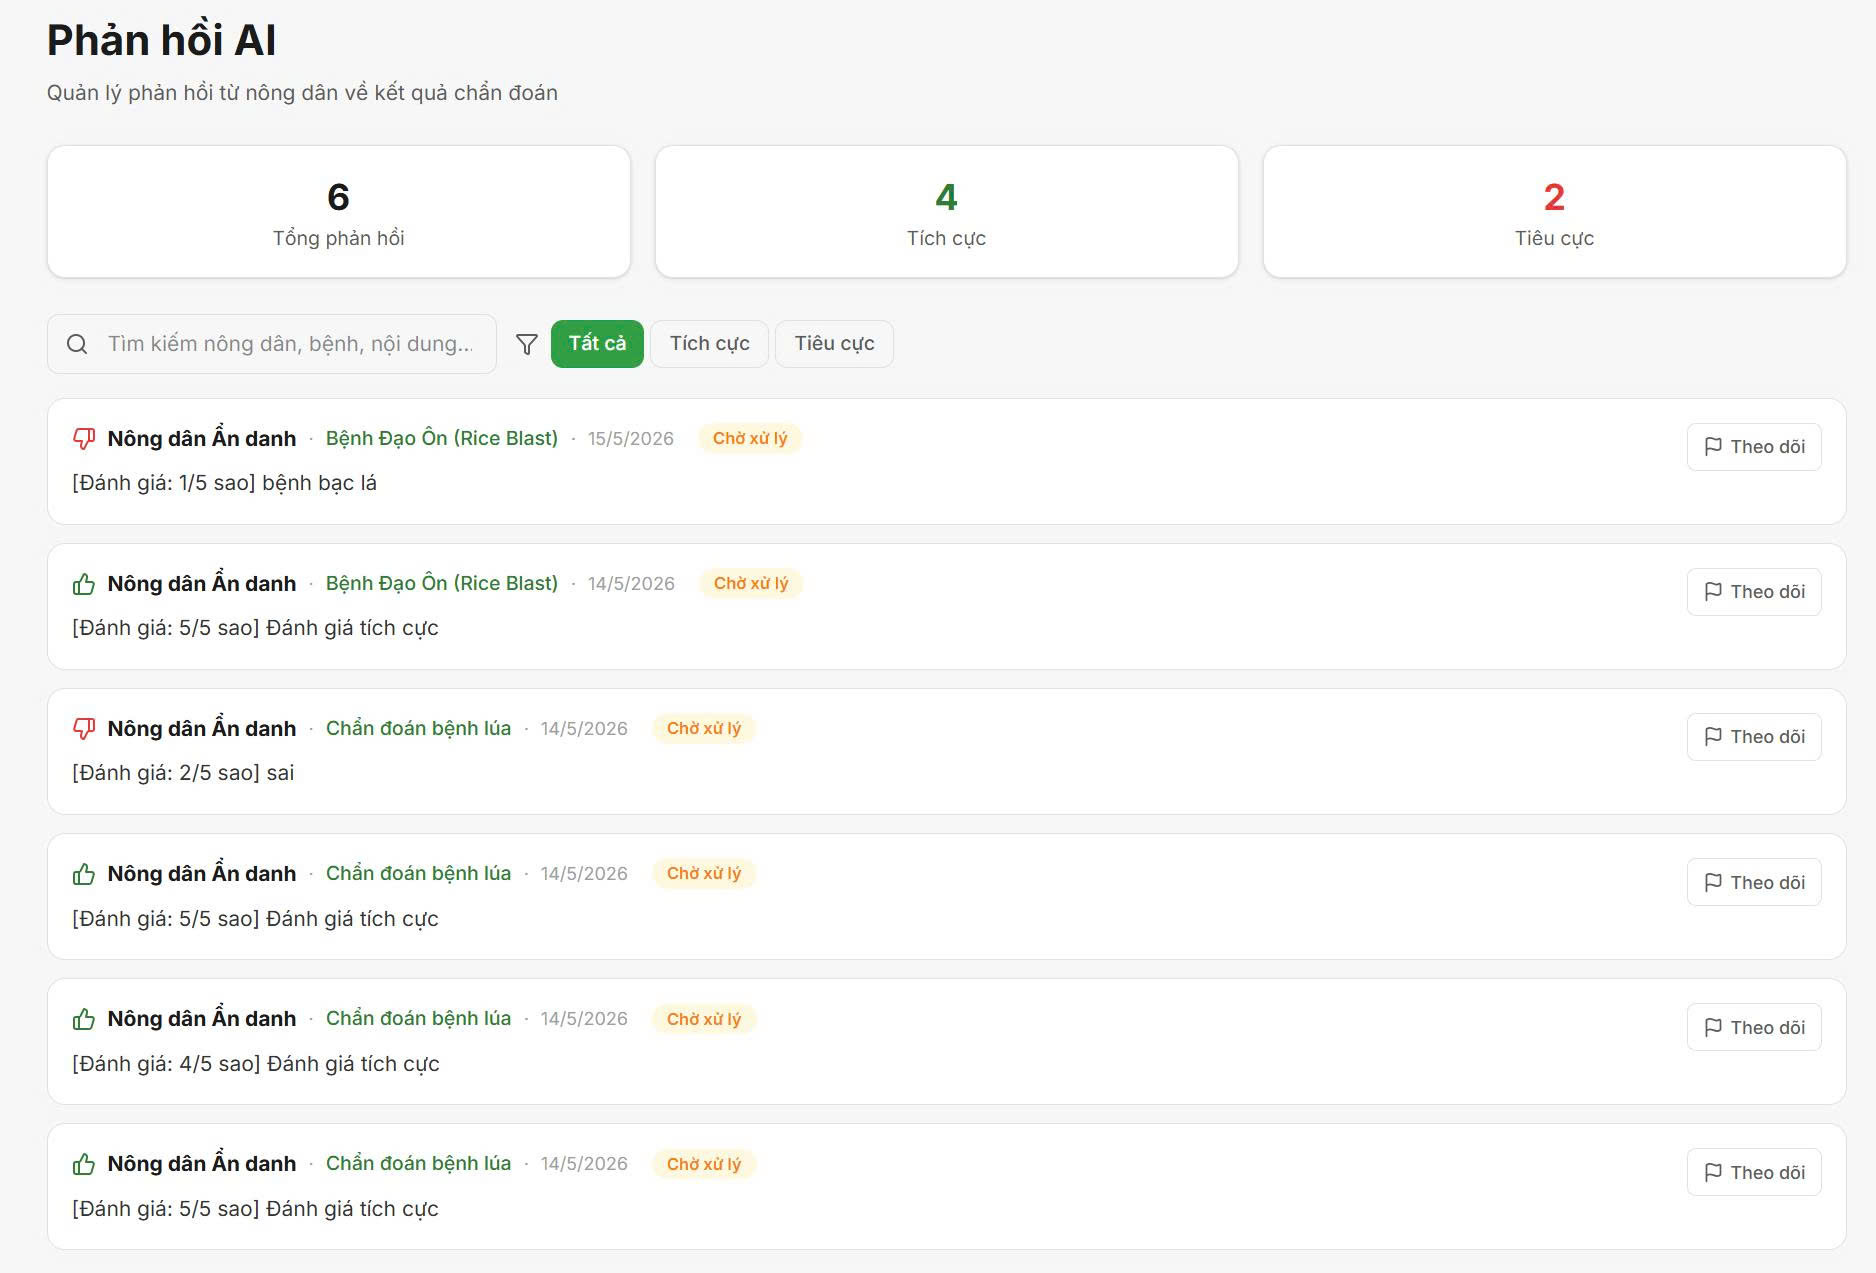
\includegraphics[width=\textwidth,height=0.75\textheight,keepaspectratio]{ad_bm_3.jpg}
    \caption{Giao diện AD\_BM 3: Phiếu xử lý phản hồi}
    \label{fig:ad-bm-3}
\end{figure}

\vspace{0.3cm}
\noindent\textbf{AD\_BM 4: BÁO CÁO HIỆU SUẤT AI}

\begin{figure}[H]
    \centering
    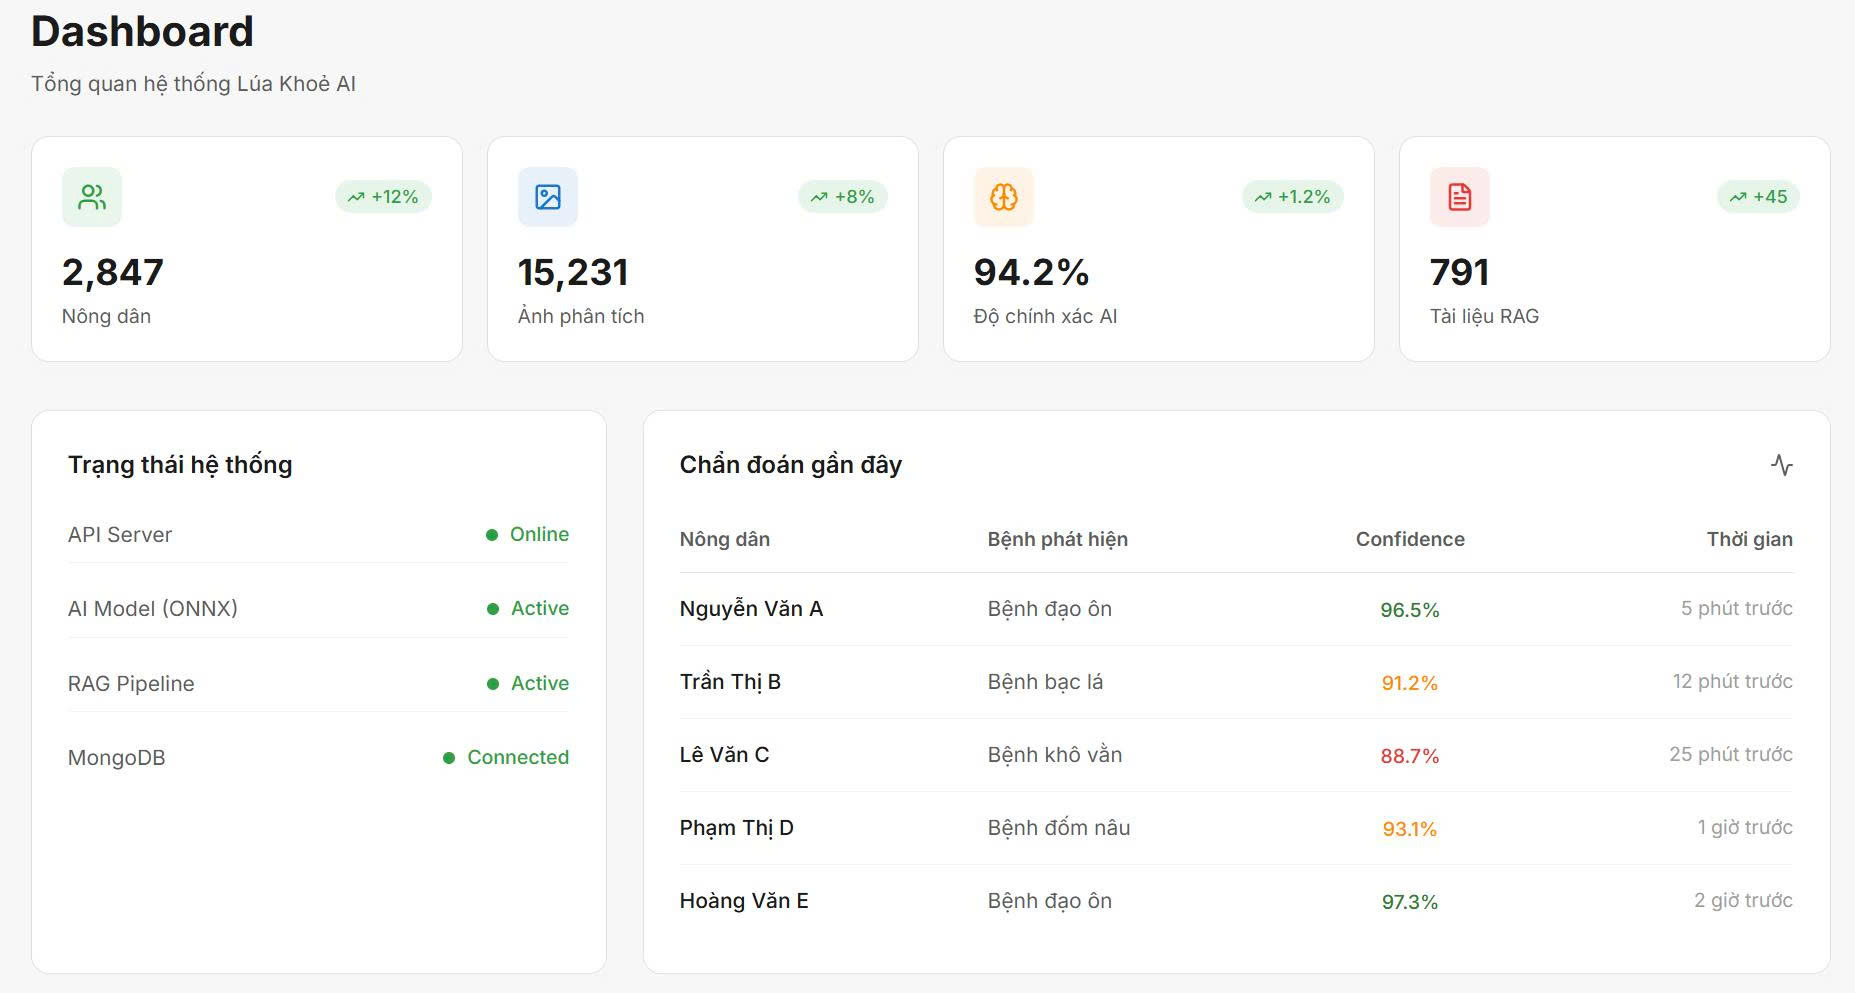
\includegraphics[width=\textwidth,height=0.75\textheight,keepaspectratio]{ad_bm_4.jpg}
    \caption{Giao diện AD\_BM 4: Báo cáo hiệu suất AI}
    \label{fig:ad-bm-4}
\end{figure}

\hrulefill

% ============================================================
\subsubsection{Xác định yêu cầu chức năng hệ thống và yêu cầu chất lượng}

\textbf{Bảng yêu cầu chức năng hệ thống:}
\begin{longtable}{|c|l|p{9.5cm}|l|}
    \hline
    \rowcolor{headerblue}
    \textbf{STT} & \textbf{Nội dung}  & \textbf{Mô tả chi tiết}                                                                            & \textbf{Ghi chú} \\
    \hline
    \endhead
    1            & Tích hợp thời tiết & Truy xuất dữ liệu thời tiết dựa trên tọa độ thực tế của nông dân để cung cấp bối cảnh môi trường.  &                  \\
    \hline
    2            & Quản lý tri thức   & Hệ thống đồng bộ các hướng dẫn dinh dưỡng để AI có thể tư vấn linh hoạt.                           &                  \\
    \hline
    3            & Bảo mật dữ liệu    & Mật khẩu được bảo mật an toàn. Toàn bộ ảnh và dữ liệu thực tế được lưu trữ phục vụ tái huấn luyện. &                  \\
    \hline
    4            & Gửi mã xác thực    & Tự động gửi mã xác thực qua email cho các luồng xác minh tài khoản.                                &                  \\
    \hline
\end{longtable}

\textbf{Bảng yêu cầu về chất lượng hệ thống:}
\begin{longtable}{|c|l|l|p{6.5cm}|l|}
    \hline
    \rowcolor{headerblue}
    \textbf{STT} & \textbf{Nội dung} & \textbf{Tiêu chuẩn} & \textbf{Mô tả chi tiết}                                                    & \textbf{Ghi chú} \\
    \hline
    \endhead
    1            & Cập nhật mô hình  & Tiến hóa            & Có thể thay thế mô hình nhận diện mới mà không làm gián đoạn người dùng.   &                  \\
    \hline
    2            & Tính tiện dụng    & Tiện dụng           & Giao diện tối ưu cho thiết bị di động, thông báo rõ ràng bằng tiếng Việt.  &                  \\
    \hline
    3            & Tốc độ xử lý      & Hiệu quả            & Phản hồi kết quả chẩn đoán trong vòng 5--7 giây.                           &                  \\
    \hline
    4            & Độ tương thích    & Tương thích         & Hoạt động ổn định trên các trình duyệt phổ biến của điện thoại thông minh. &                  \\
    \hline
    5            & Tính kịp thời     & Hiệu quả            & Mã xác thực gửi đến người dùng trong vòng 30 giây.                         &                  \\
    \hline
\end{longtable}

\hrulefill

% ============================================================
\section{Biểu đồ Use Case}

\subsection{Biểu đồ Use Case tổng quát}

% Chèn ảnh Use Case tổng quát (xuất từ Mermaid/draw.io)
\begin{figure}[htbp]
    \centering
    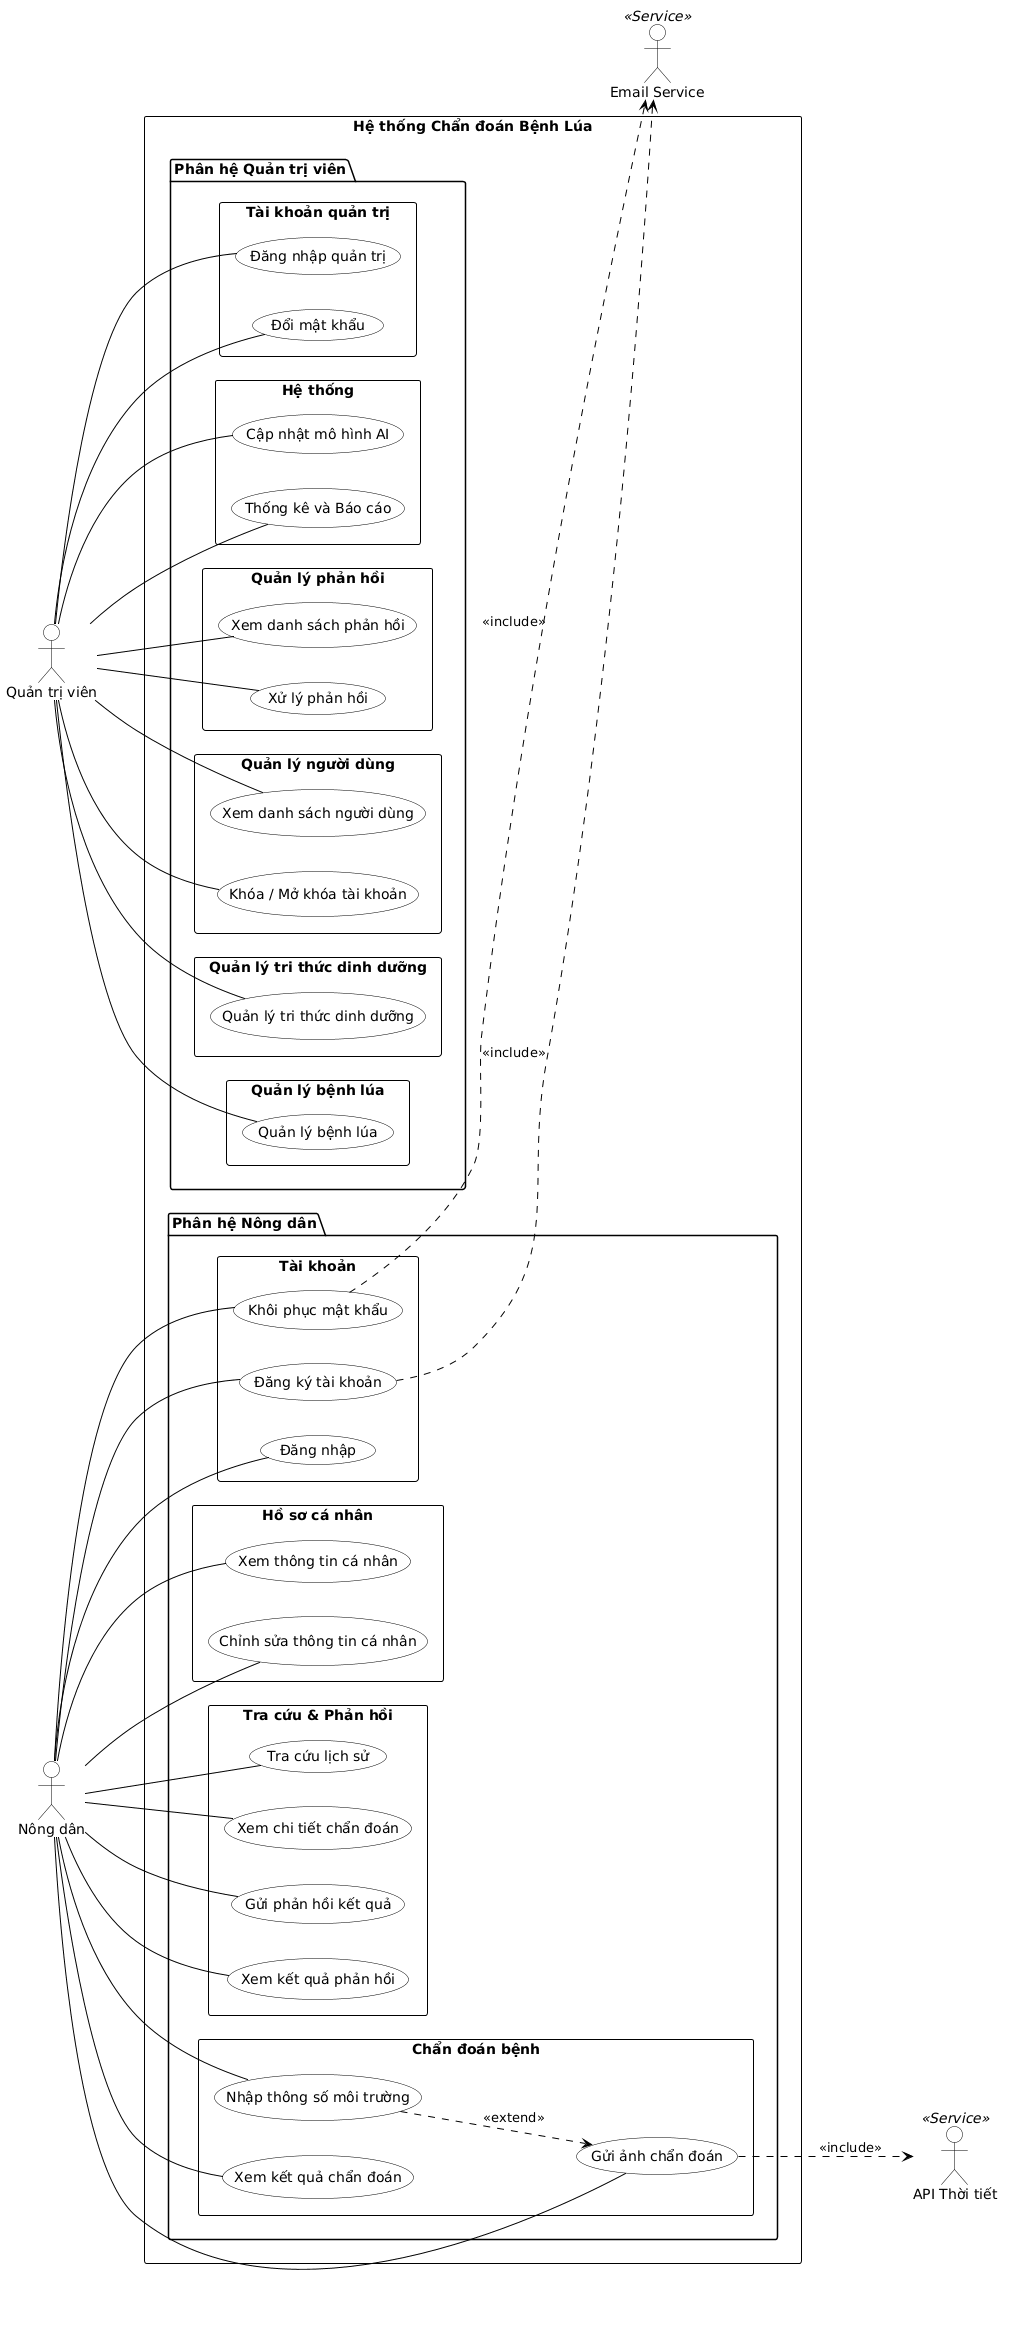
\includegraphics[width=\textwidth,height=0.85\textheight,keepaspectratio]{usecase-tong-quat.png}
    \caption{Biểu đồ Use Case tổng quát của hệ thống}
    \label{fig:usecase-tong-quat}
\end{figure}

\subsection{Bảng ký hiệu UML}

\begin{longtable}{|l|p{11cm}|}
    \hline
    \rowcolor{headerblue}
    \textbf{Ký hiệu}                       & \textbf{Ý nghĩa}                            \\
    \hline
    Hình người (stick figure)              & Actor --- tác nhân tương tác với hệ thống   \\
    \hline
    Hình elip                              & Use Case --- chức năng hệ thống             \\
    \hline
    Hình chữ nhật bao quanh                & System Boundary --- ranh giới hệ thống      \\
    \hline
    Đường liền                             & Association --- actor sử dụng use case      \\
    \hline
    Mũi tên đứt nét + \texttt{<<include>>} & Use case bắt buộc gọi đến use case khác     \\
    \hline
    Mũi tên đứt nét + \texttt{<<extend>>}  & Use case mở rộng (tùy chọn, không bắt buộc) \\
    \hline
\end{longtable}

\hrulefill

% ============================================================
\section{Biểu đồ tuần tự (Sequence Diagrams)}

\subsection{SD-01: Đăng ký tài khoản (có xác thực email)}
% \noindent\textit{[Chèn ảnh SD-01 tại đây]}
\begin{figure}[htbp]
    \centering
    \includegraphics[width=\textwidth,height=0.85\textheight,keepaspectratio]{sd-01-register.png}
    \caption{Biểu đồ tuần tự: Đăng ký tài khoản}
    \label{fig:sd-01}
\end{figure}

\subsection{SD-02: Đăng nhập hệ thống}
% \noindent\textit{[Chèn ảnh SD-02 tại đây]}
\begin{figure}[htbp]
    \centering
    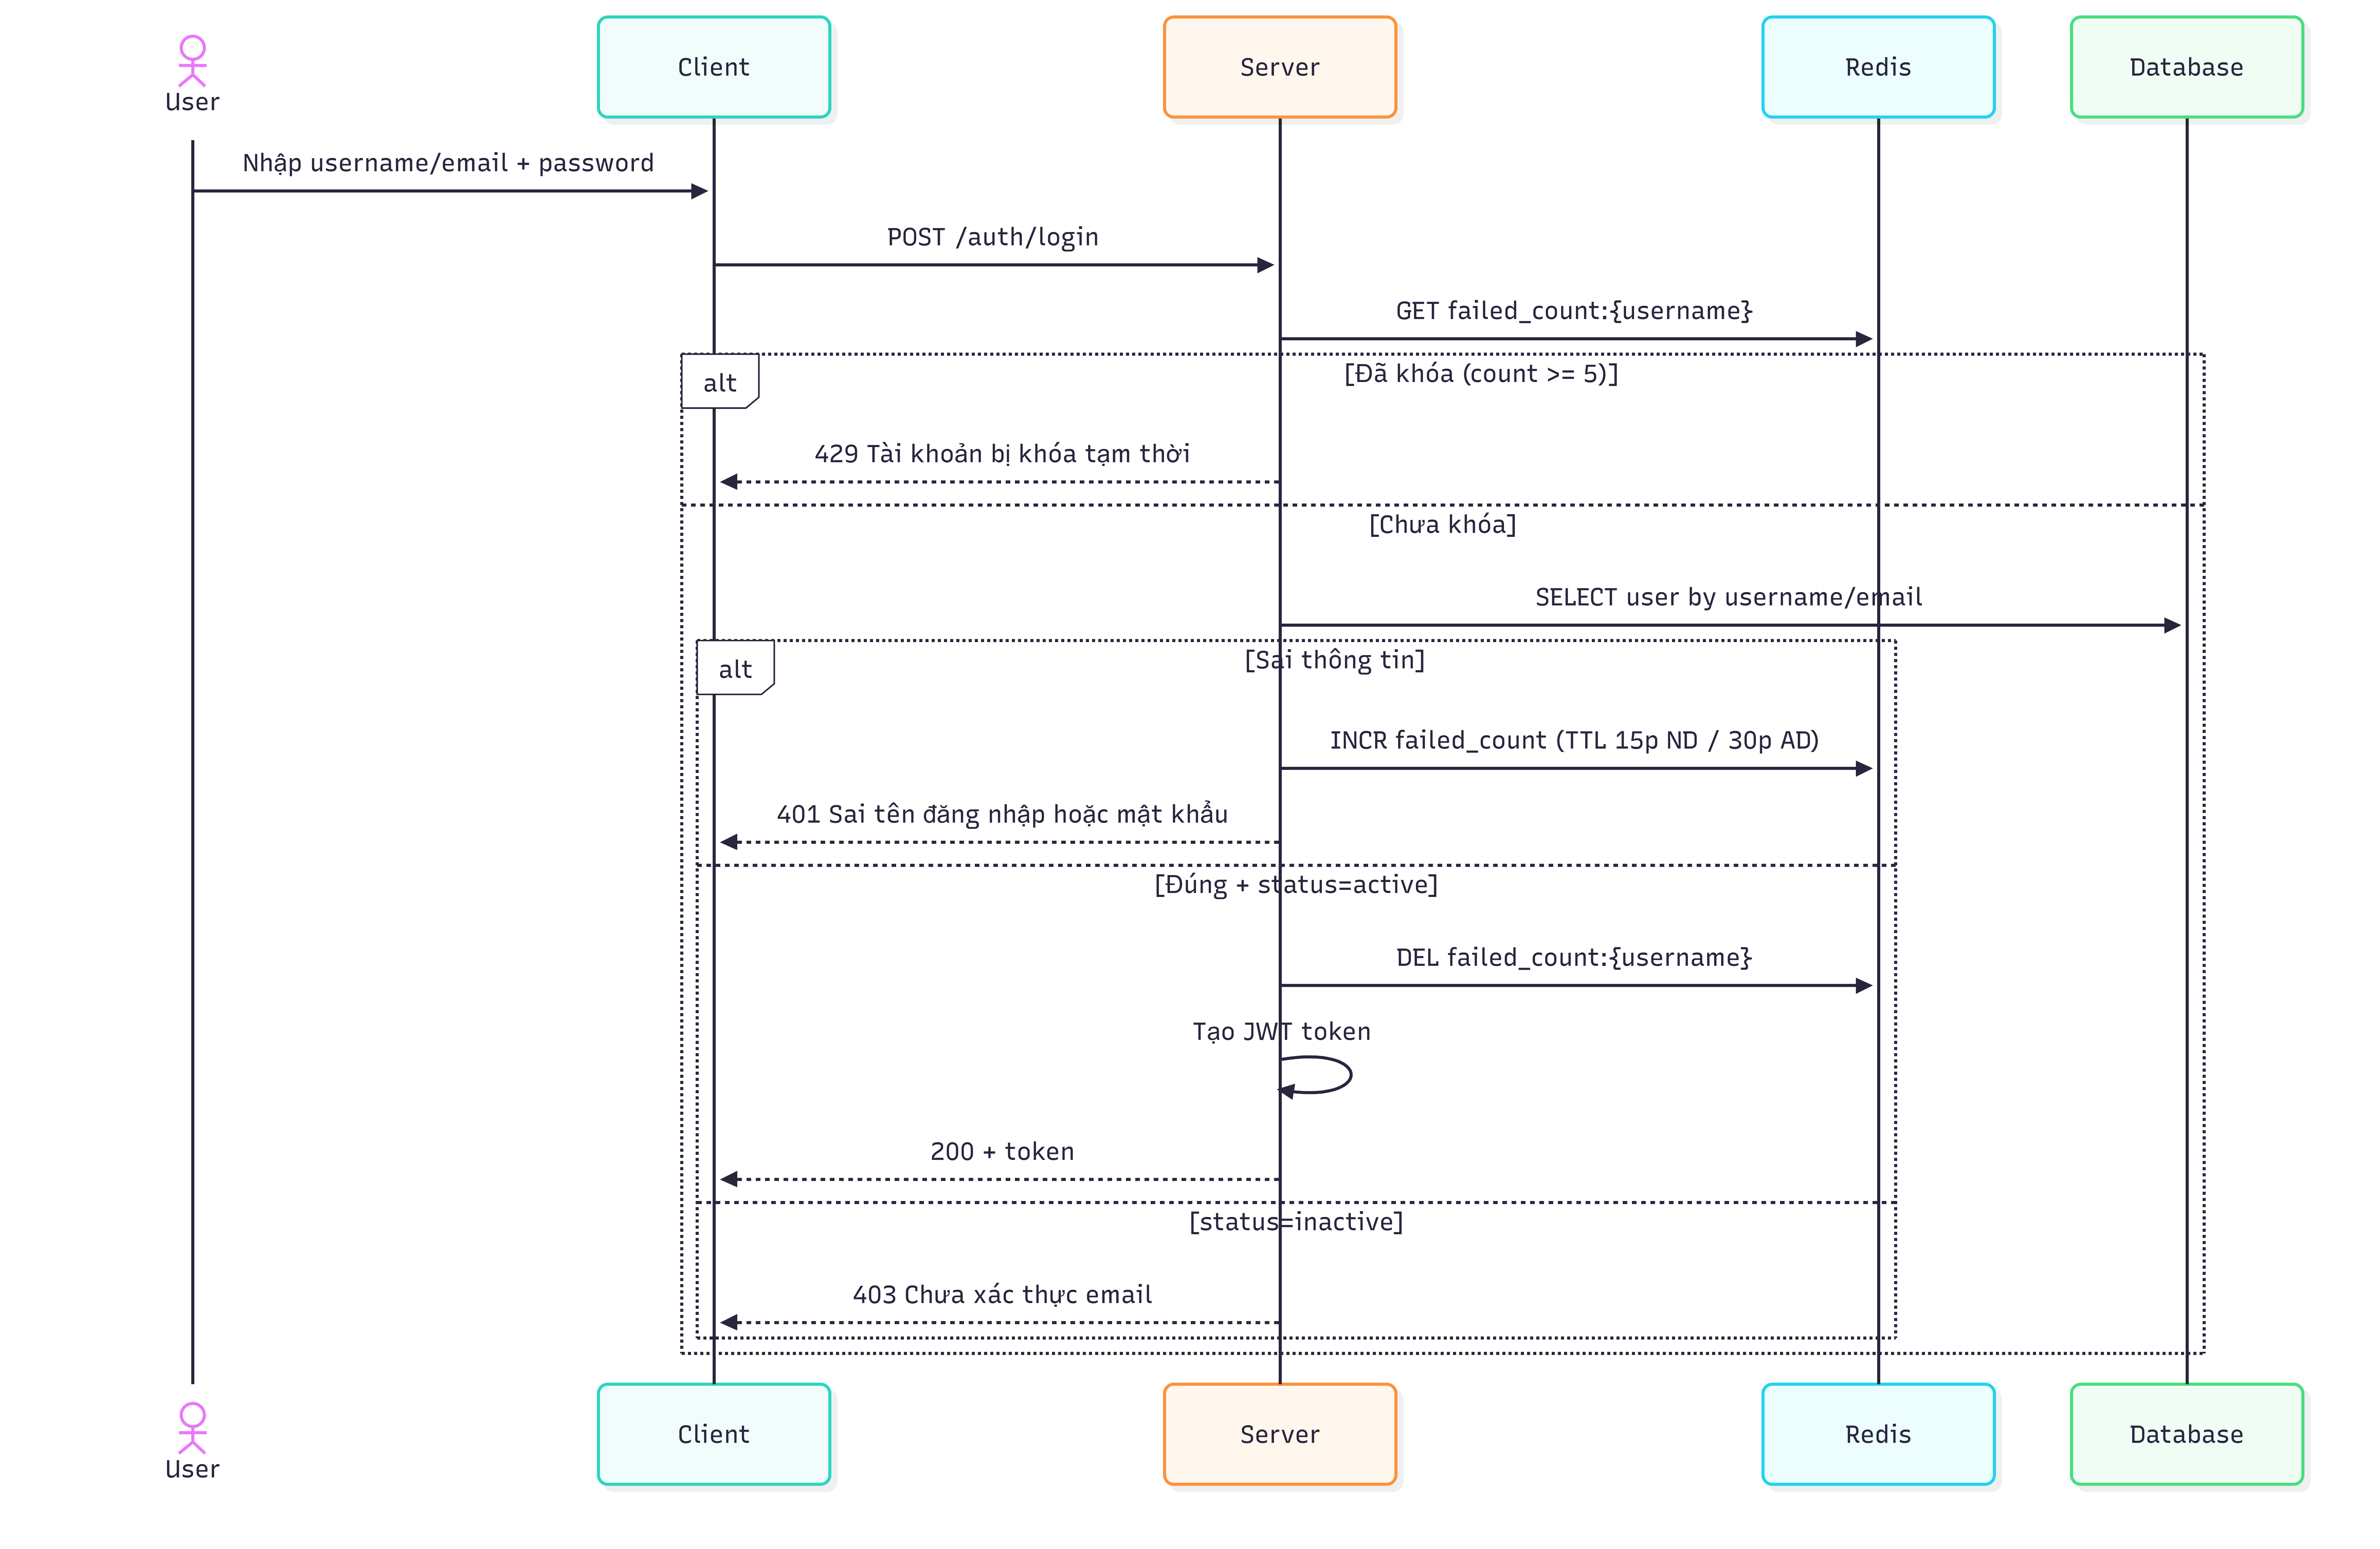
\includegraphics[width=\textwidth,height=0.85\textheight,keepaspectratio]{sd-02-login.png}
    \caption{Biểu đồ tuần tự: Đăng nhập hệ thống}
    \label{fig:sd-02}
\end{figure}

\subsection{SD-03: Khôi phục mật khẩu}
% \noindent\textit{[Chèn ảnh SD-03 tại đây]}
\begin{figure}[htbp]
    \centering
    \includegraphics[width=\textwidth,height=0.85\textheight,keepaspectratio]{sd-03-forgot-password.png}
    \caption{Biểu đồ tuần tự: Khôi phục mật khẩu}
    \label{fig:sd-03}
\end{figure}

\subsection{SD-04: Xem \& Chỉnh sửa hồ sơ cá nhân}
% \noindent\textit{[Chèn ảnh SD-04 tại đây]}
\begin{figure}[htbp]
    \centering
    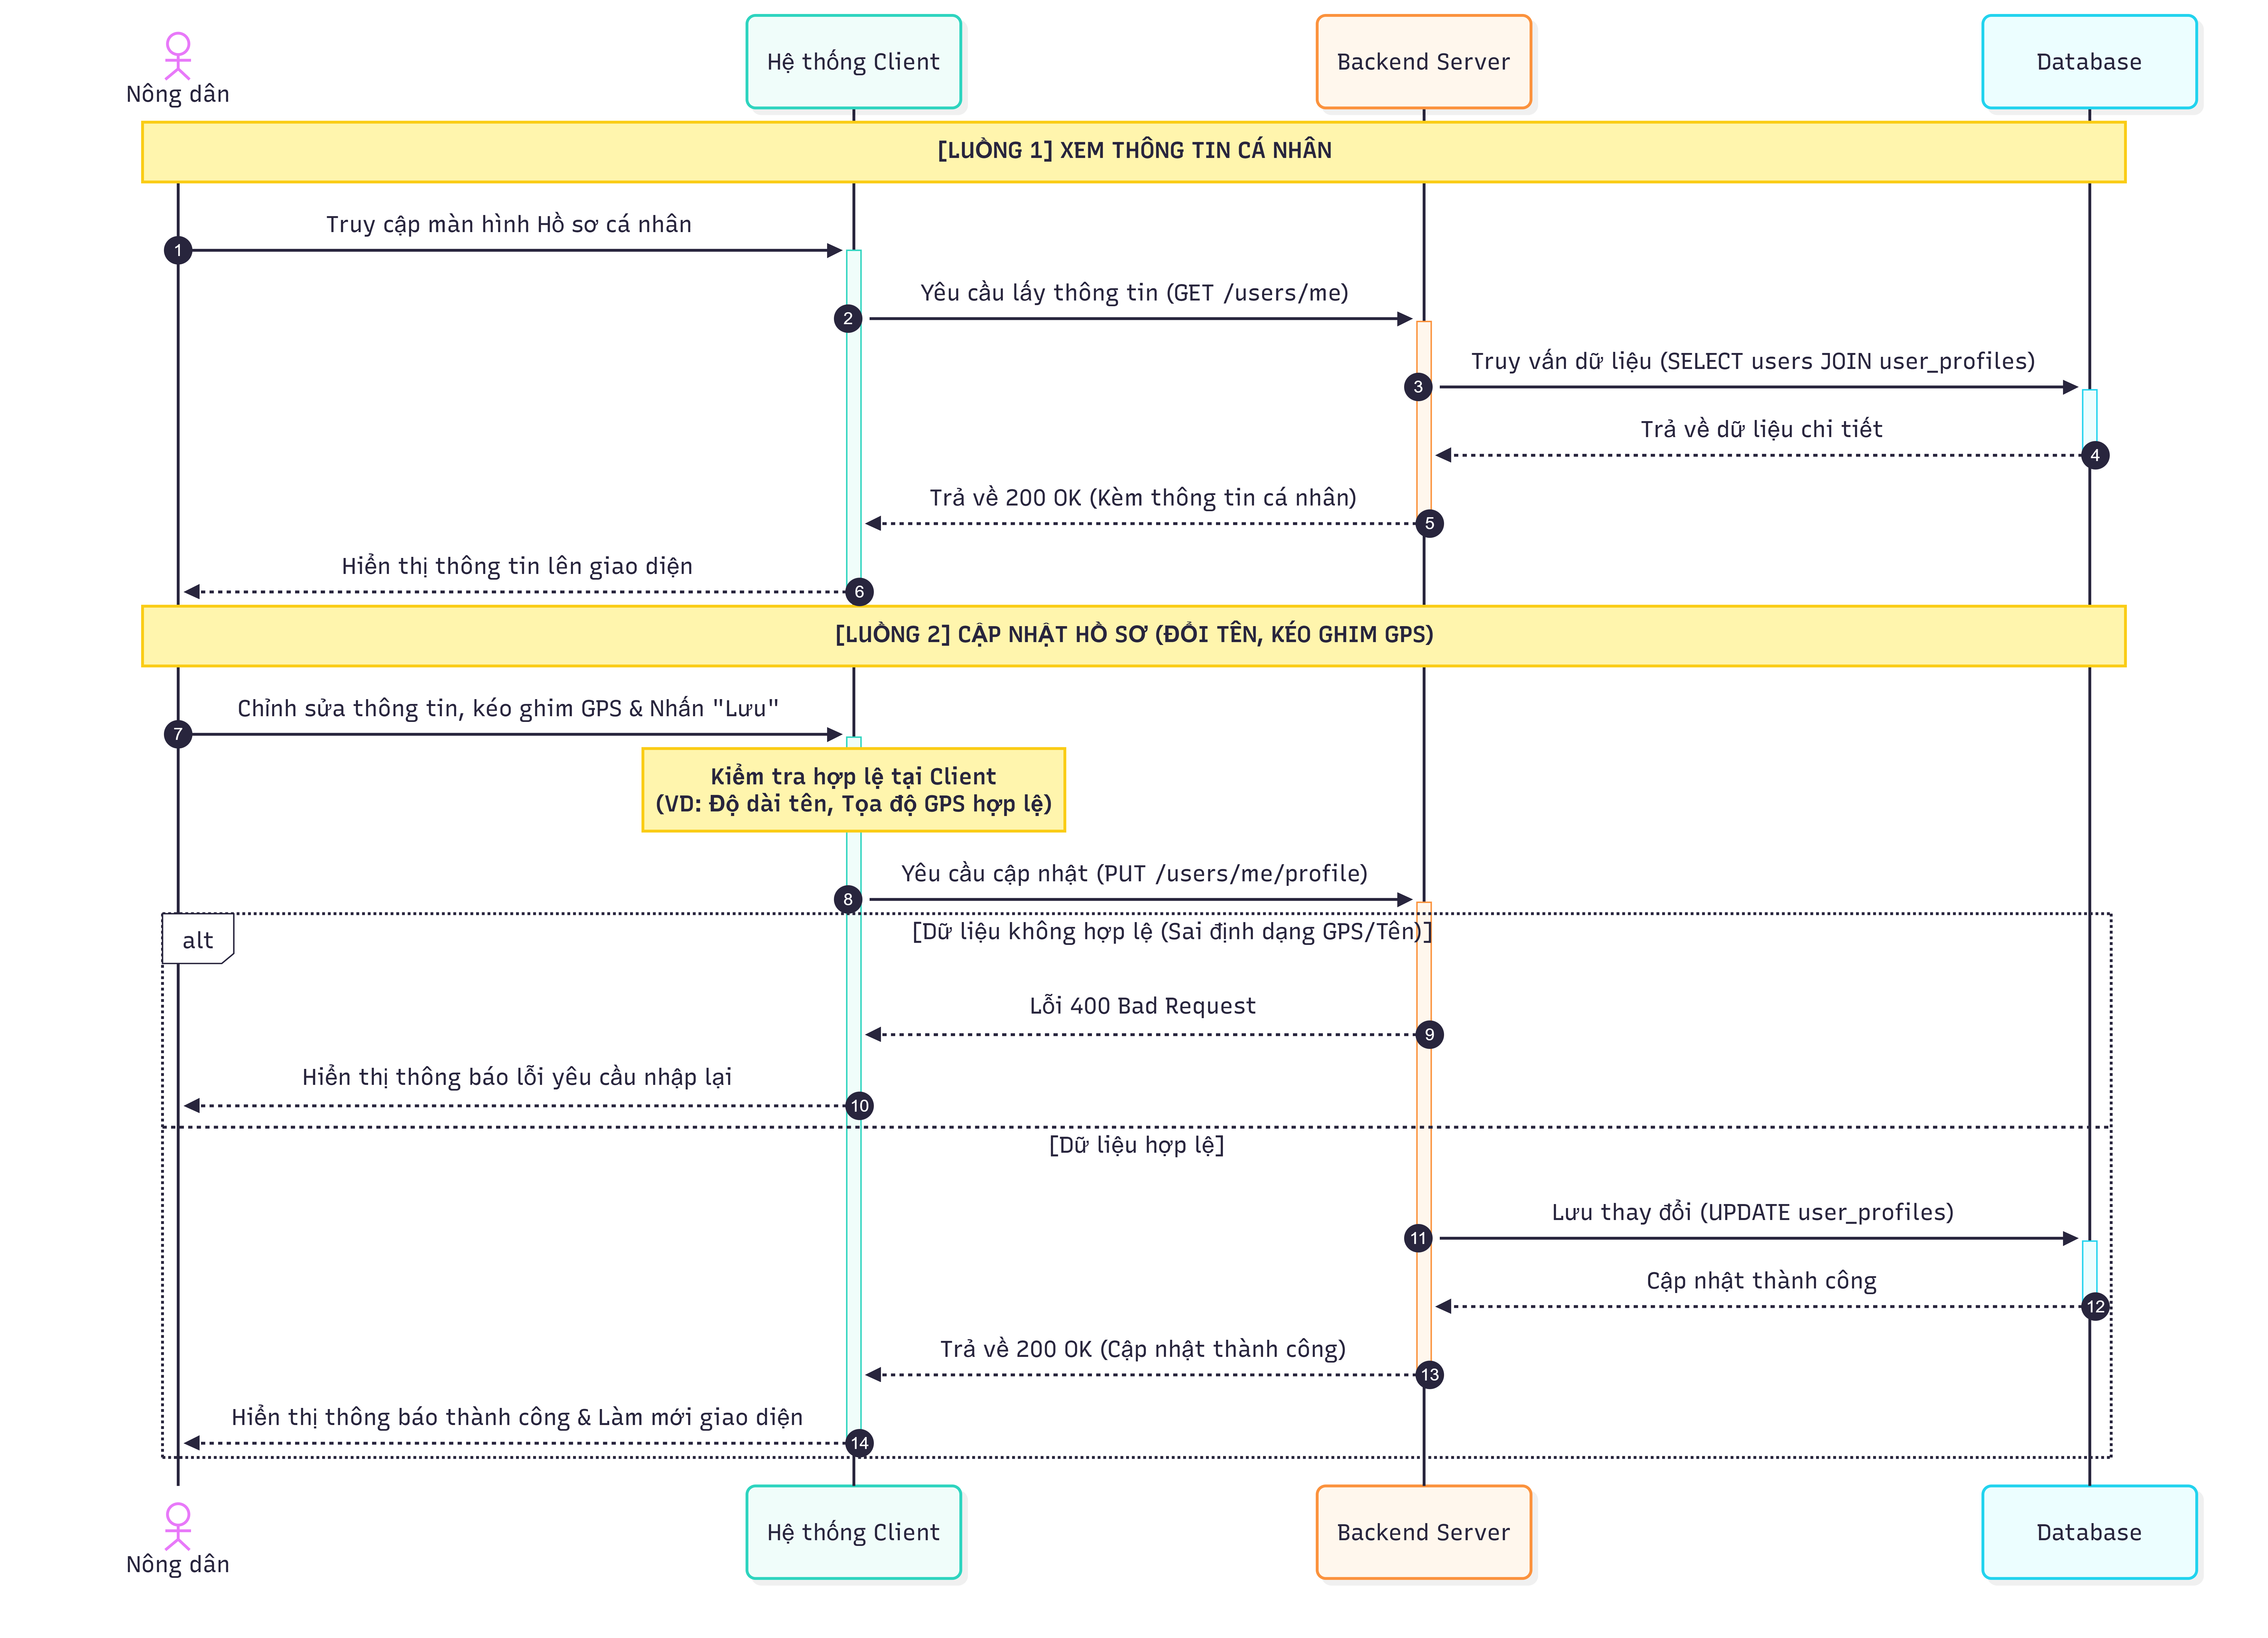
\includegraphics[width=\textwidth,height=0.85\textheight,keepaspectratio]{sd-04-profile.png}
    \caption{Biểu đồ tuần tự: Xem và chỉnh sửa hồ sơ cá nhân}
    \label{fig:sd-04}
\end{figure}

\subsection{SD-05: Gửi ảnh chẩn đoán (Core Flow)}
% \noindent\textit{[Chèn ảnh SD-05 tại đây]}
\begin{figure}[htbp]
    \centering
    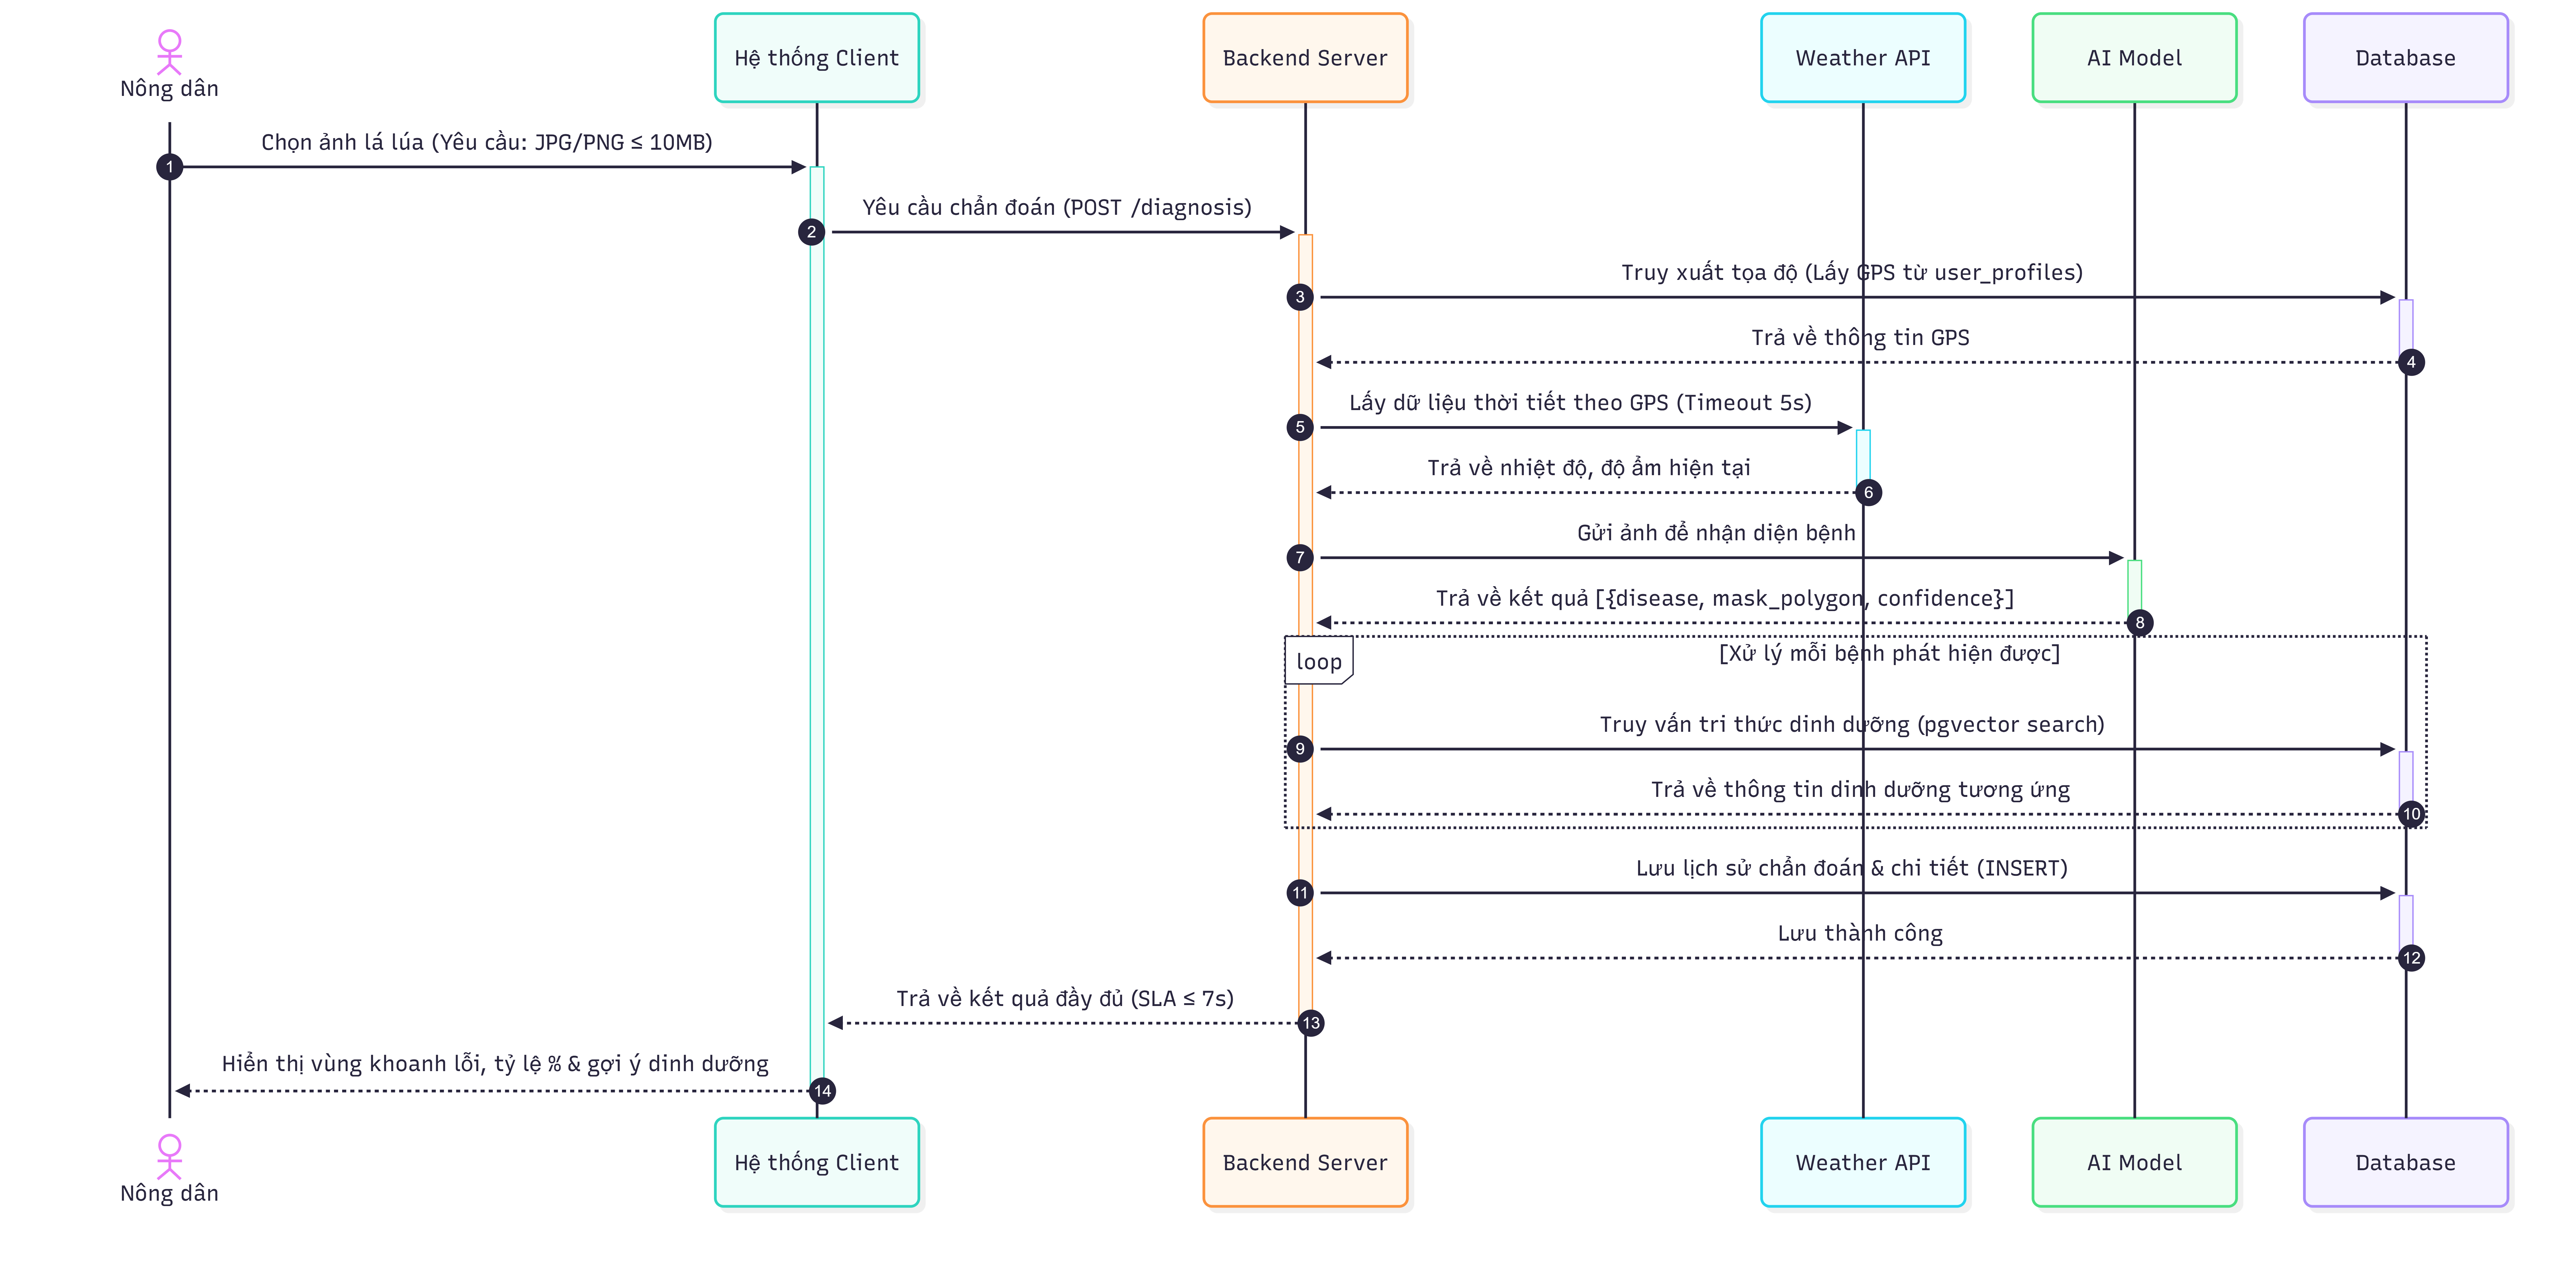
\includegraphics[width=\textwidth,height=0.85\textheight,keepaspectratio]{sd-05-diagnosis.png}
    \caption{Biểu đồ tuần tự: Gửi ảnh chẩn đoán}
    \label{fig:sd-05}
\end{figure}

\subsection{SD-06: Nhập thông số môi trường bổ sung}
% \noindent\textit{[Chèn ảnh SD-06 tại đây]}
\begin{figure}[htbp]
    \centering
    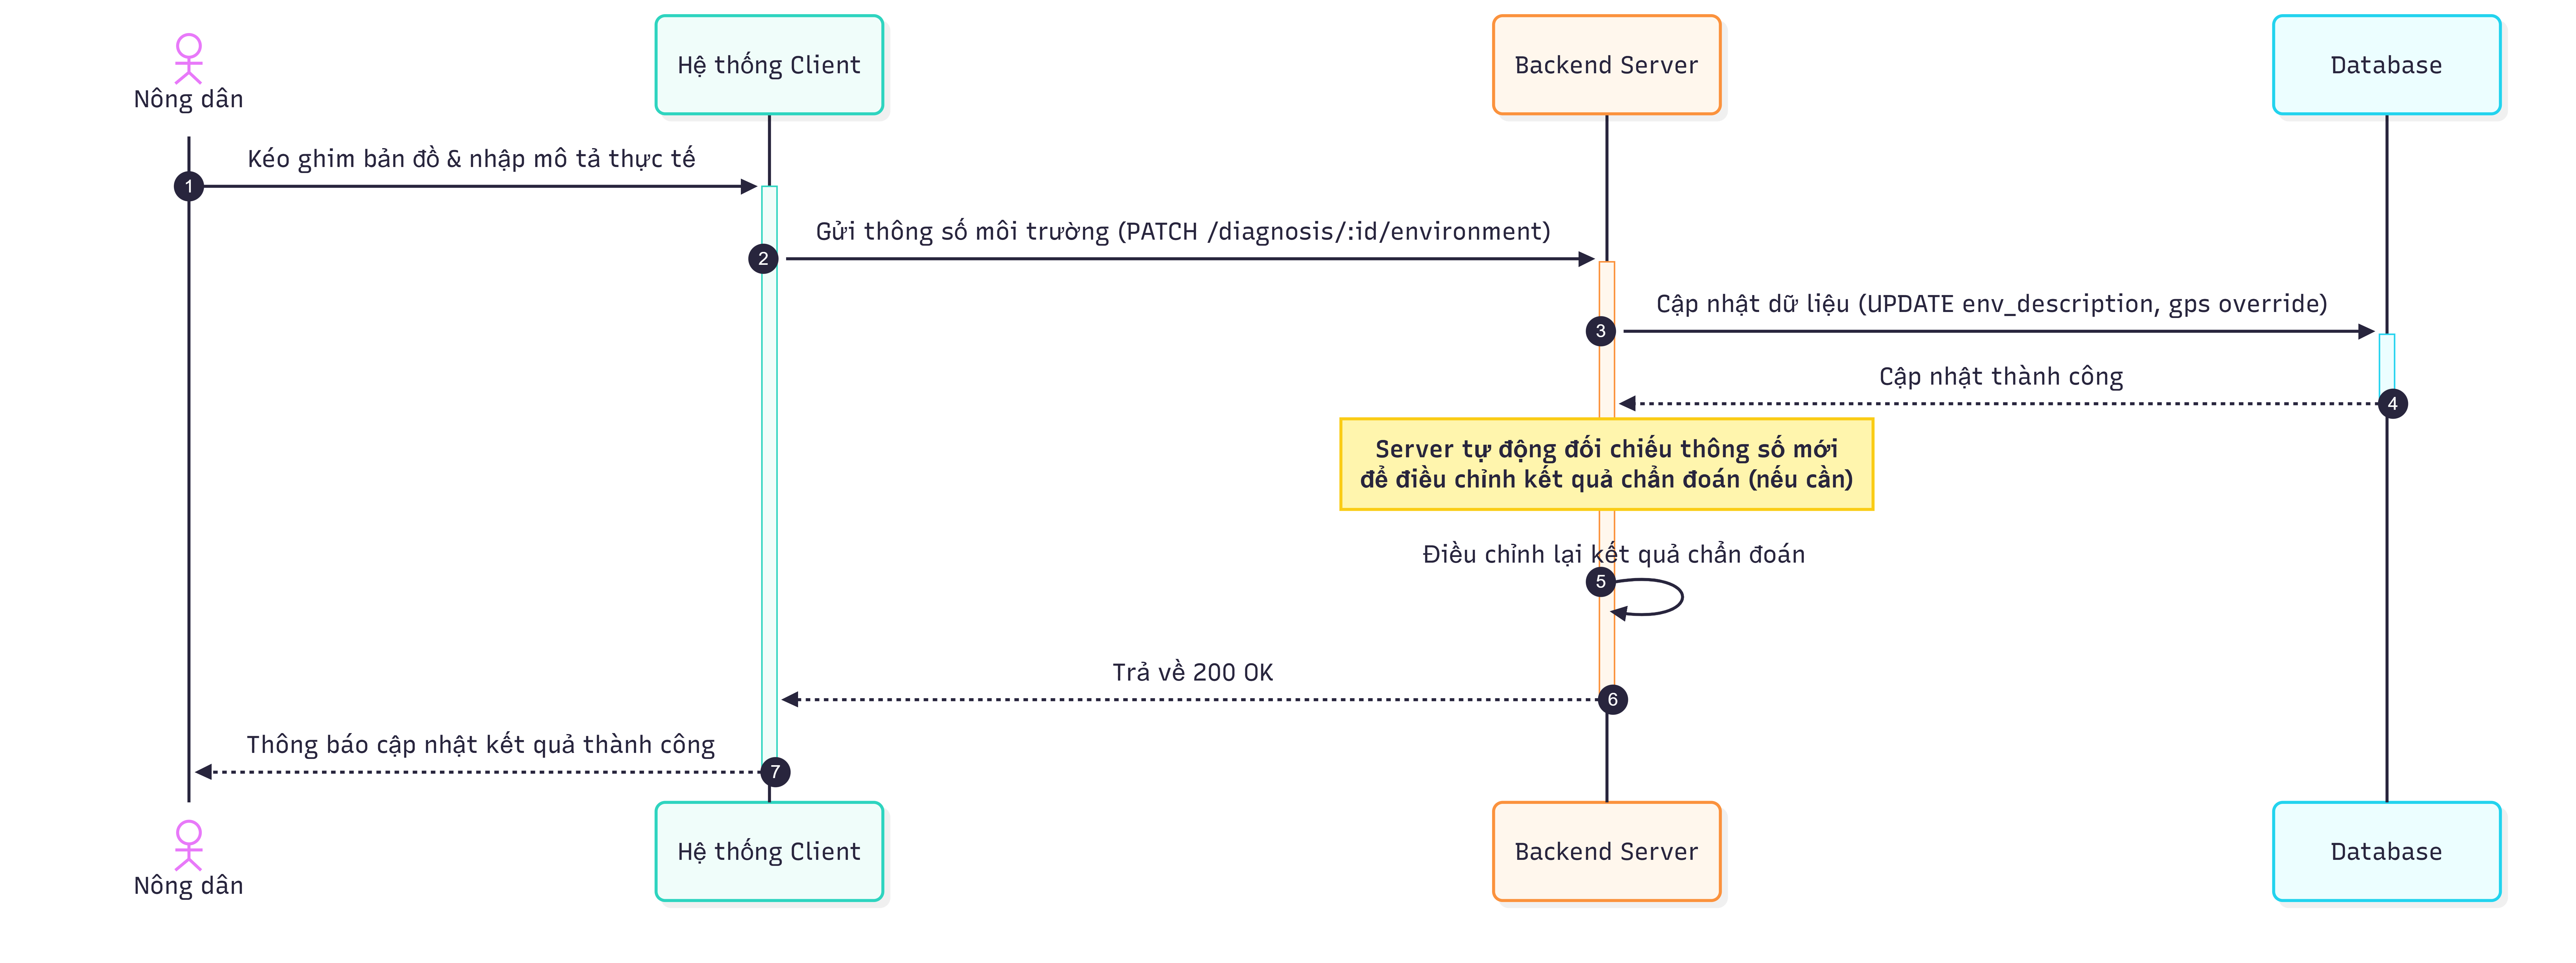
\includegraphics[width=\textwidth,height=0.85\textheight,keepaspectratio]{sd-06-environment.png}
    \caption{Biểu đồ tuần tự: Nhập thông số môi trường bổ sung}
    \label{fig:sd-06}
\end{figure}

\subsection{SD-07: Tra cứu lịch sử \& Xem chi tiết}
% \noindent\textit{[Chèn ảnh SD-07 tại đây]}
\begin{figure}[htbp]
    \centering
    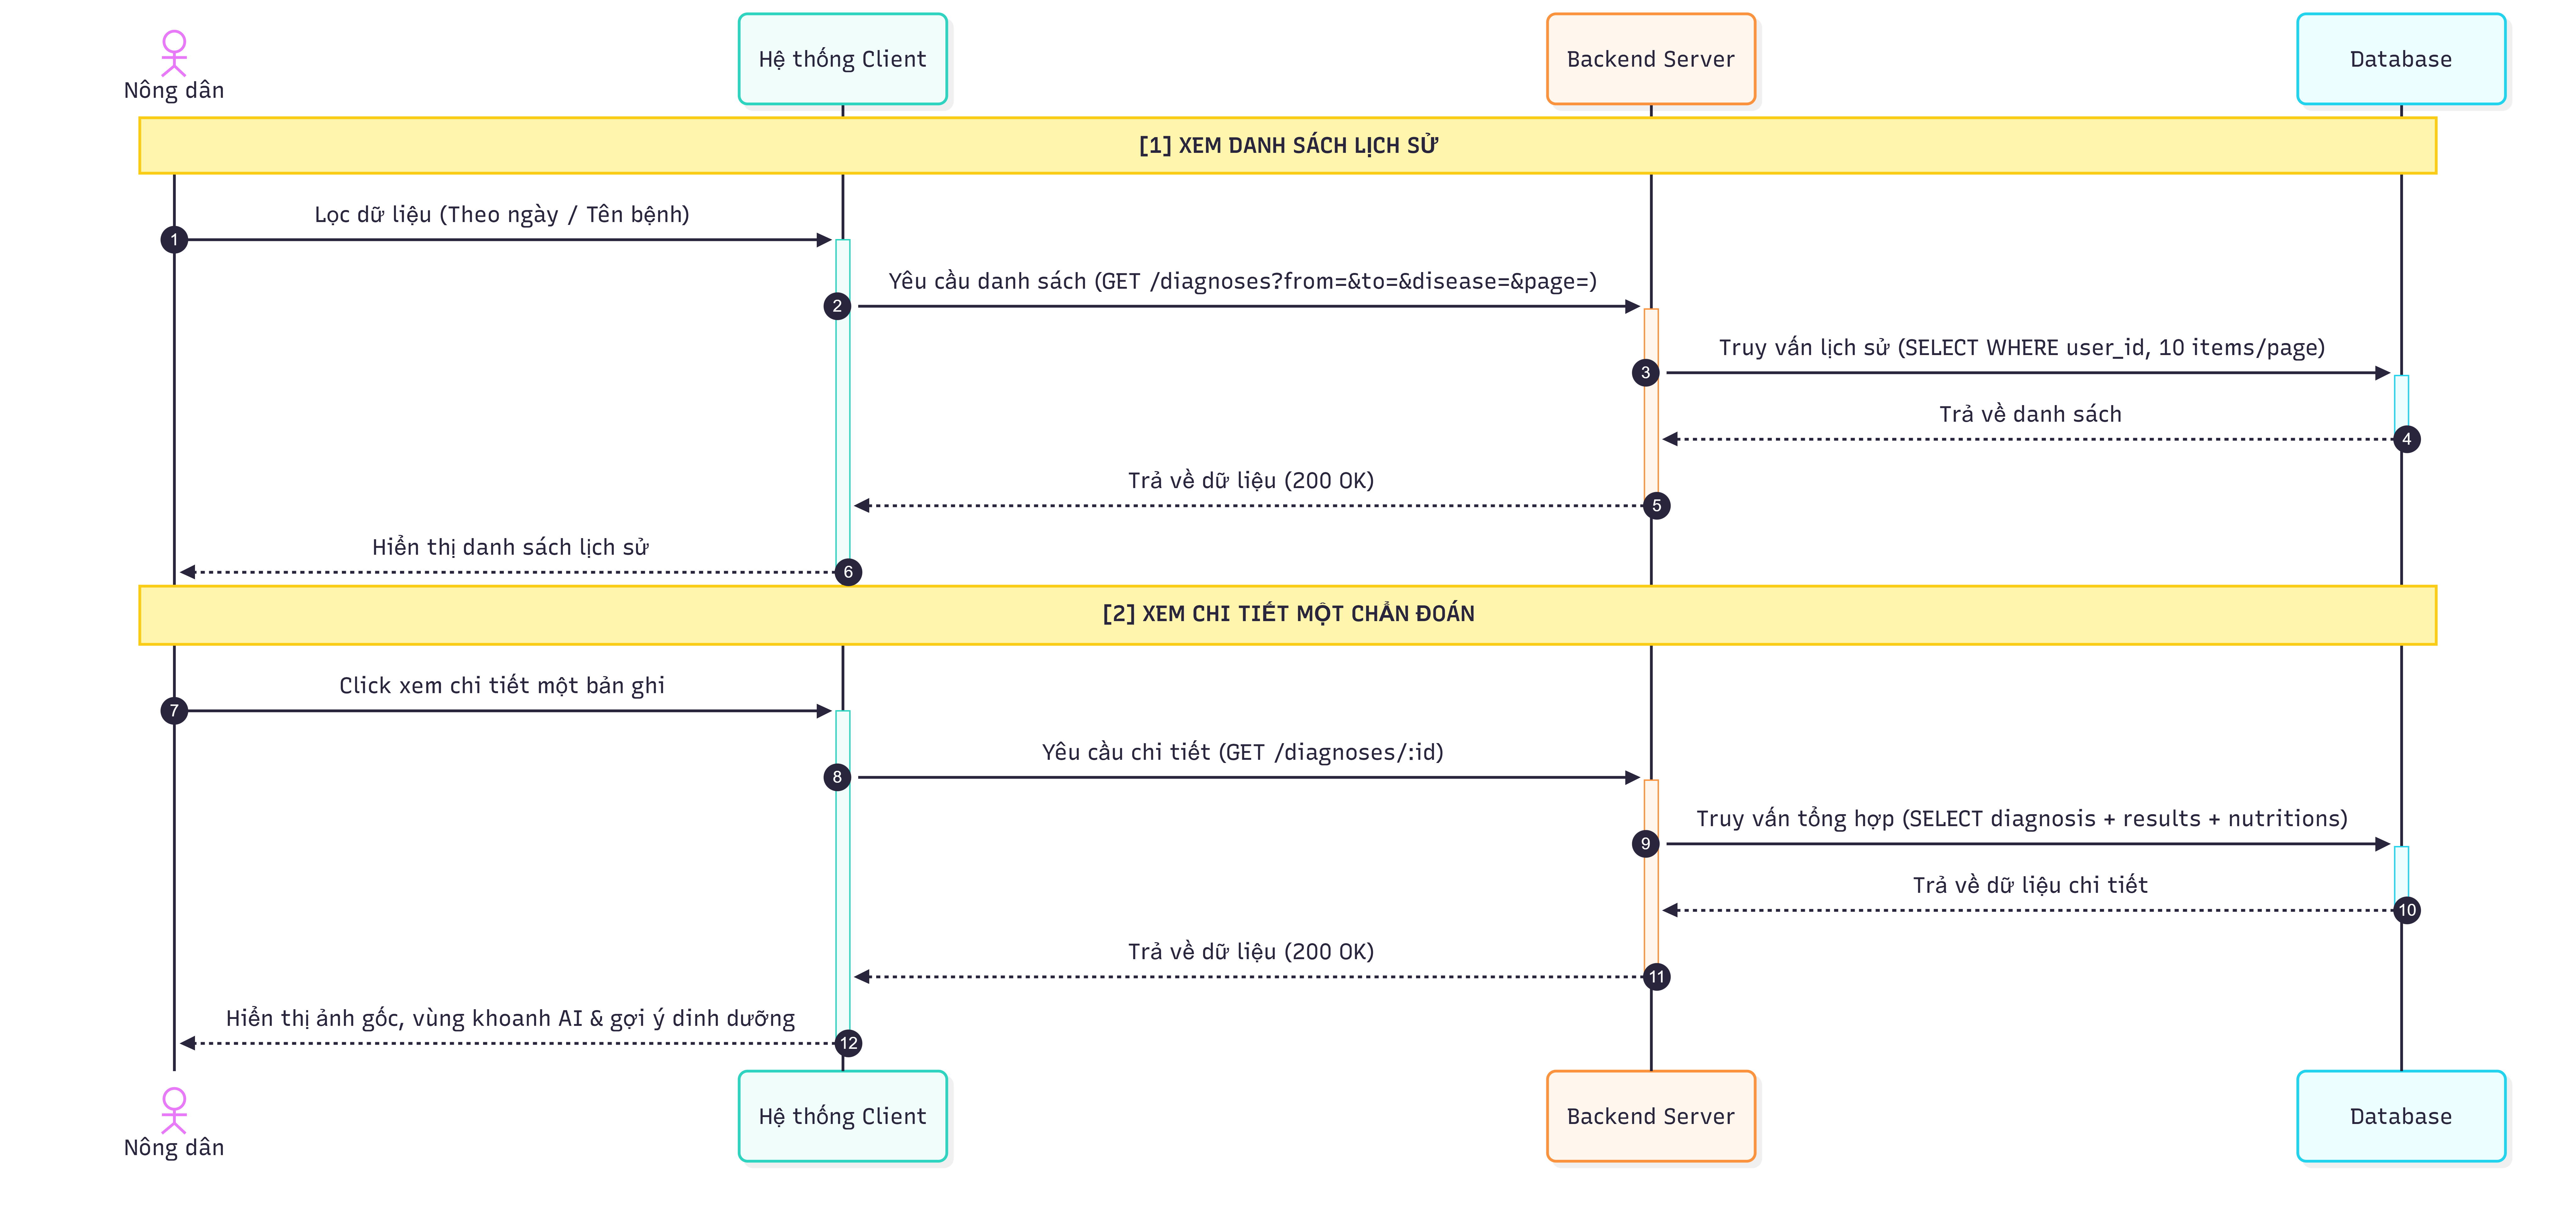
\includegraphics[width=\textwidth,height=0.85\textheight,keepaspectratio]{sd-07-history.png}
    \caption{Biểu đồ tuần tự: Tra cứu lịch sử và xem chi tiết}
    \label{fig:sd-07}
\end{figure}

\subsection{SD-08: Gửi phản hồi kết quả \& SD-09: Xem kết quả xử lý phản hồi}
% \noindent\textit{[Chèn ảnh SD-08, SD-09 tại đây]}
\begin{figure}[htbp]
    \centering
    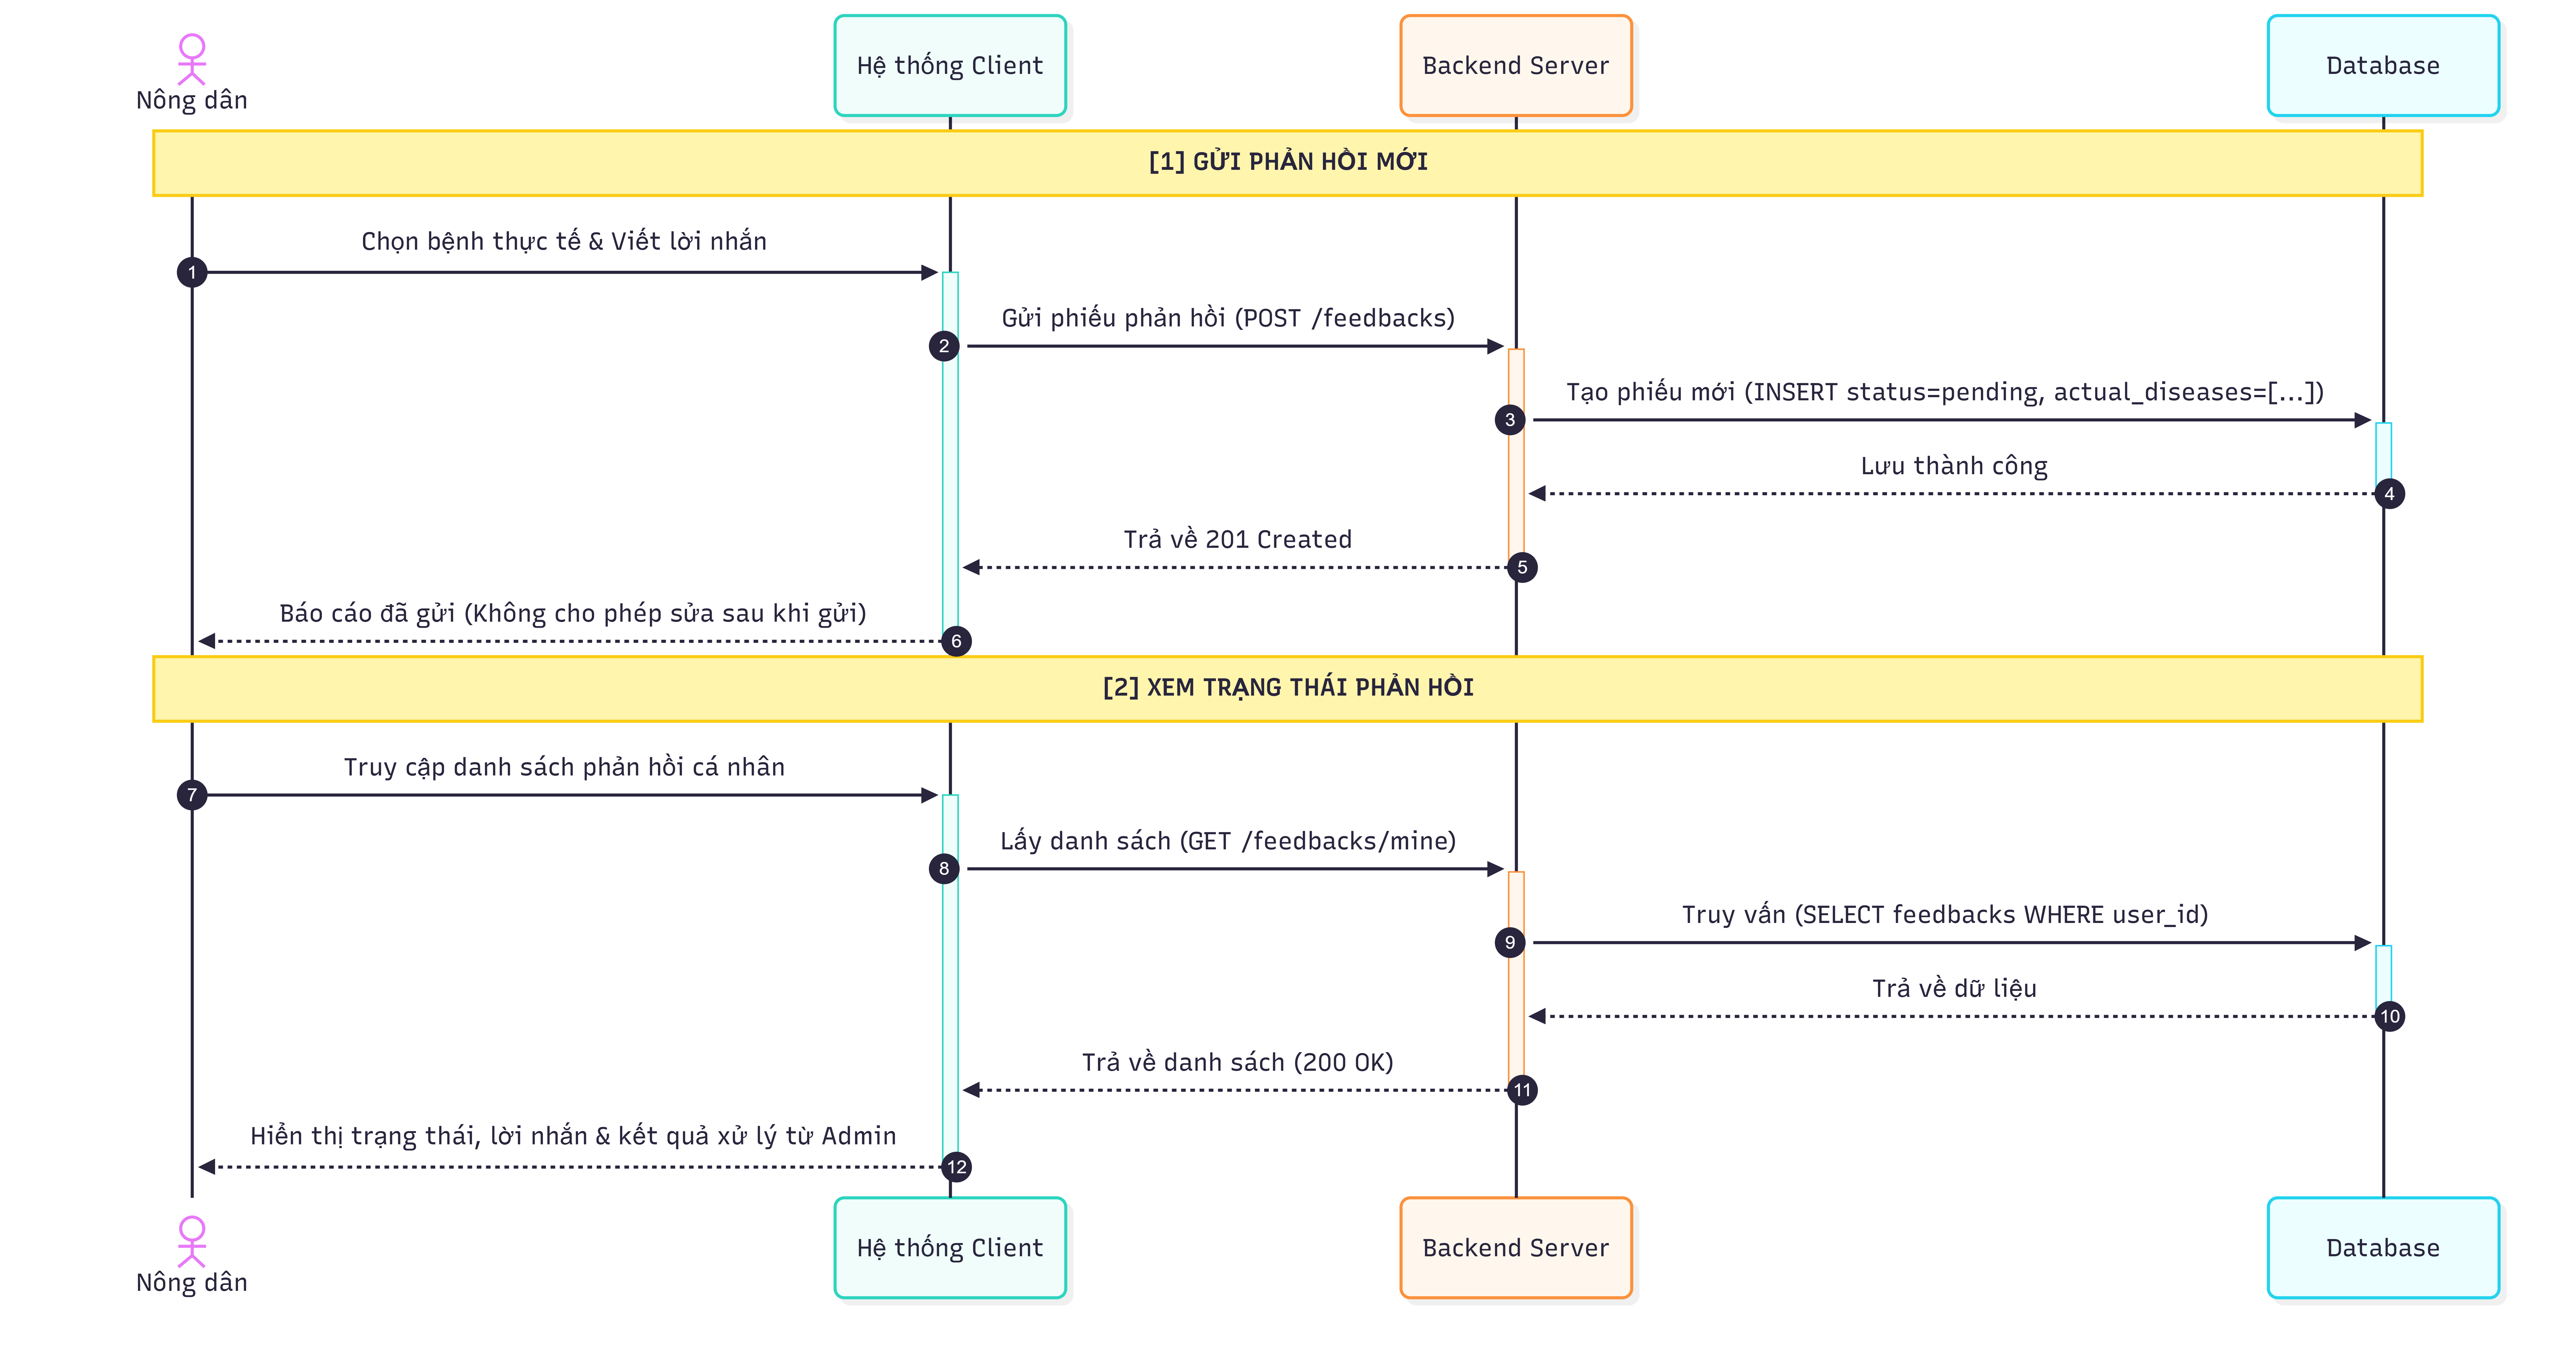
\includegraphics[width=\textwidth,height=0.85\textheight,keepaspectratio]{sd-0809-feedback.png}
    \caption{Biểu đồ tuần tự: Gửi phản hồi và xem kết quả xử lý}
    \label{fig:sd-0809}
\end{figure}

\subsection{SD-10: Quản lý bệnh lúa (CRUD)}
% \noindent\textit{[Chèn ảnh SD-10 tại đây]}
\begin{figure}[htbp]
    \centering
    \includegraphics[width=\textwidth,height=0.85\textheight,keepaspectratio]{sd-10-disease-crud.png}
    \caption{Biểu đồ tuần tự: Quản lý bệnh lúa (CRUD)}
    \label{fig:sd-10}
\end{figure}

\subsection{SD-11: Quản lý tri thức dinh dưỡng}
% \noindent\textit{[Chèn ảnh SD-11 tại đây]}
\begin{figure}[htbp]
    \centering
    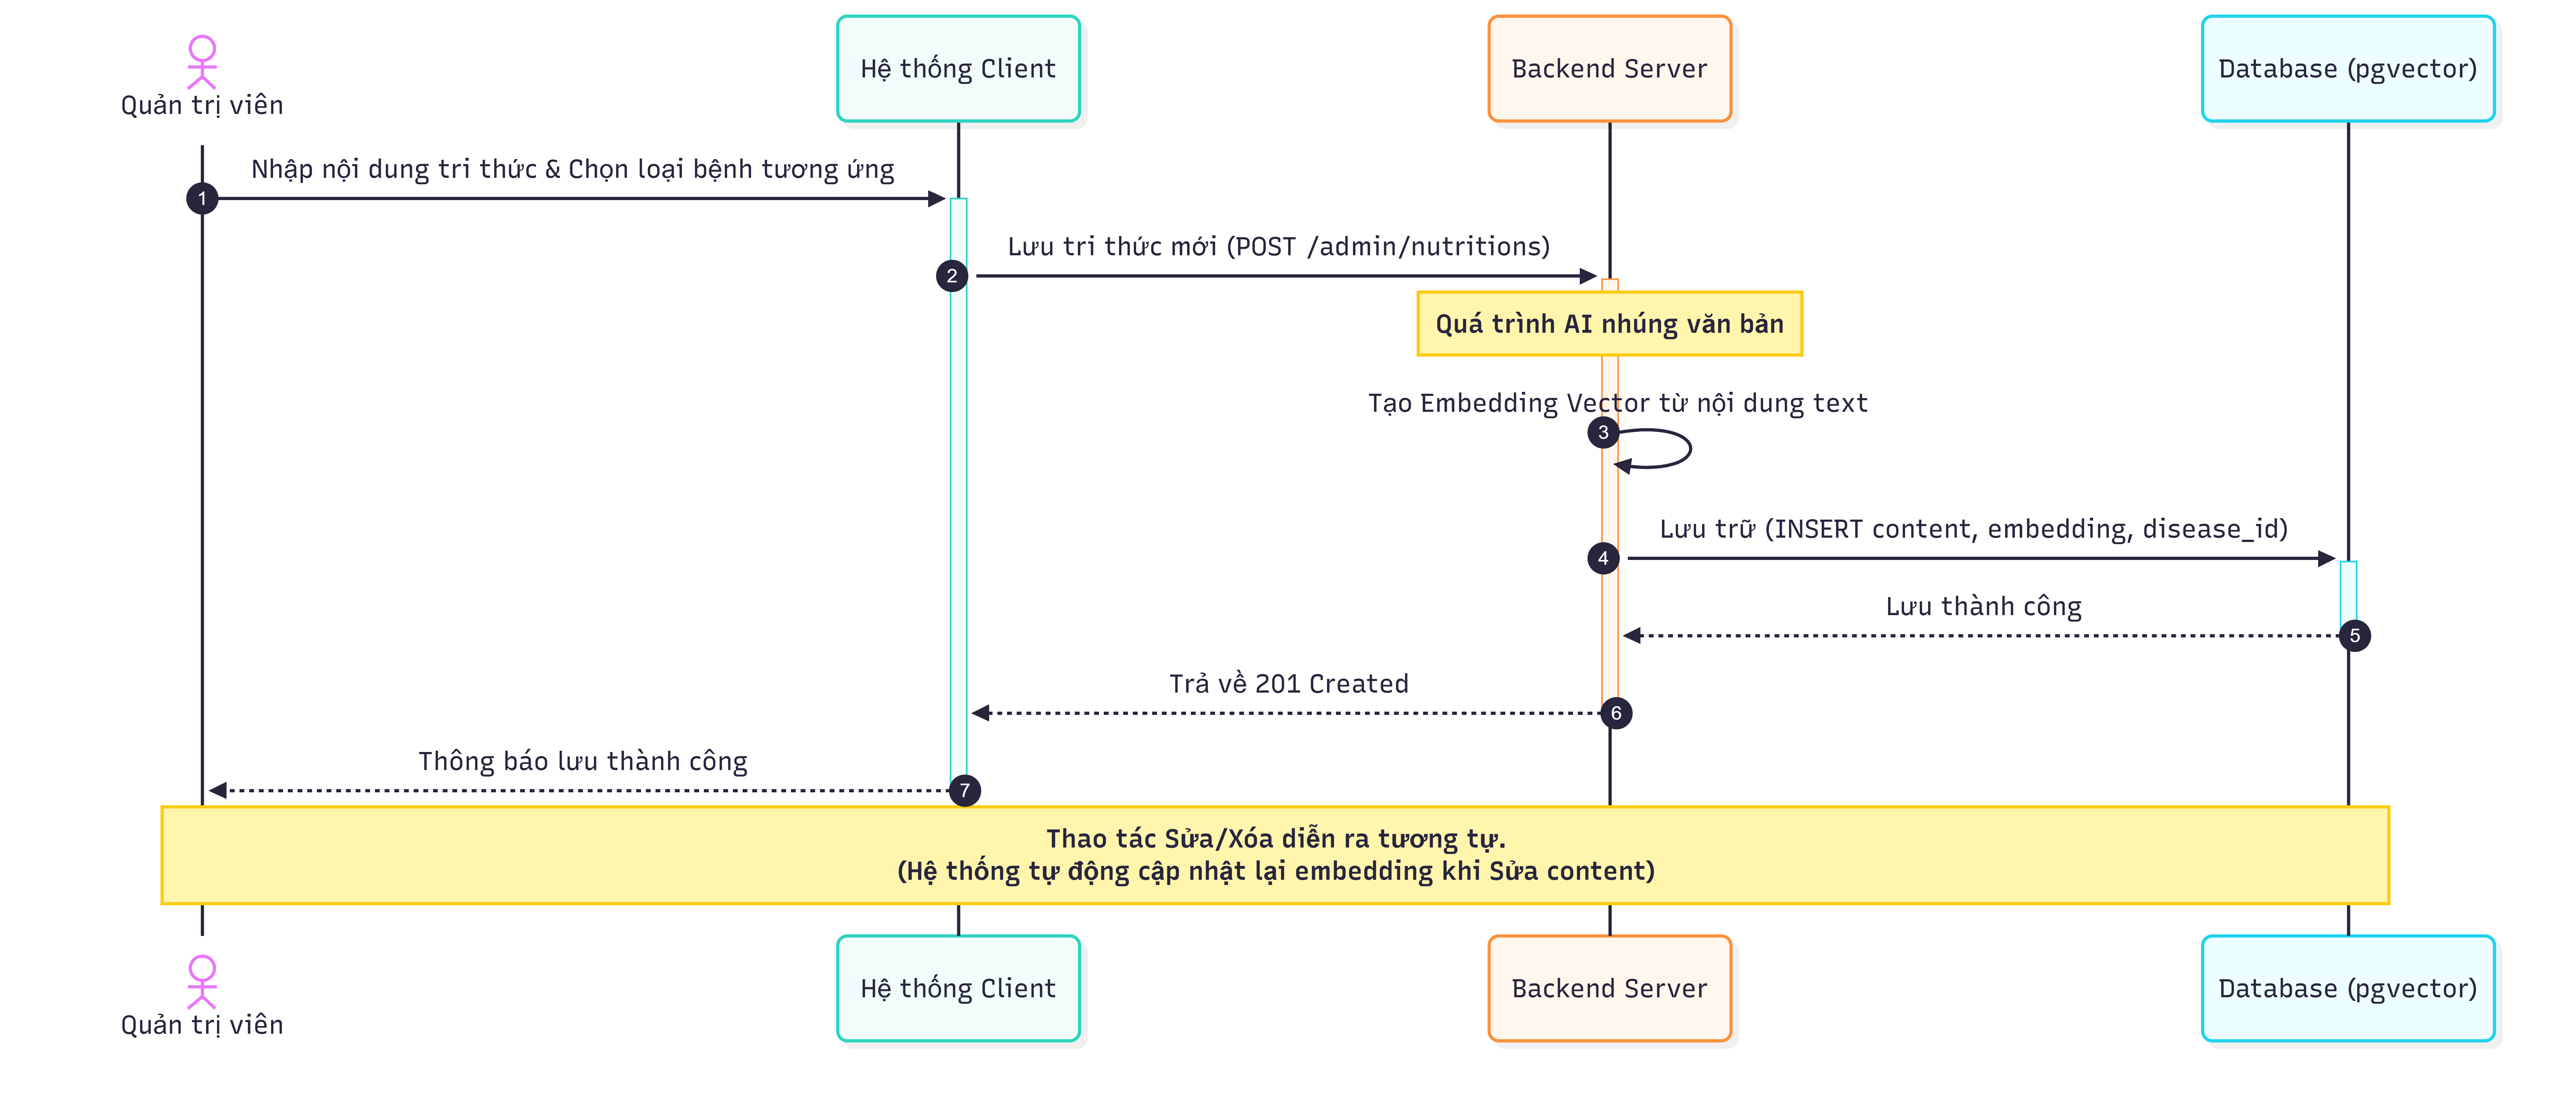
\includegraphics[width=\textwidth,height=0.85\textheight,keepaspectratio]{sd-11-nutrition.png}
    \caption{Biểu đồ tuần tự: Quản lý tri thức dinh dưỡng}
    \label{fig:sd-11}
\end{figure}

\subsection{SD-12: Quản lý người dùng}
% \noindent\textit{[Chèn ảnh SD-12 tại đây]}
\begin{figure}[htbp]
    \centering
    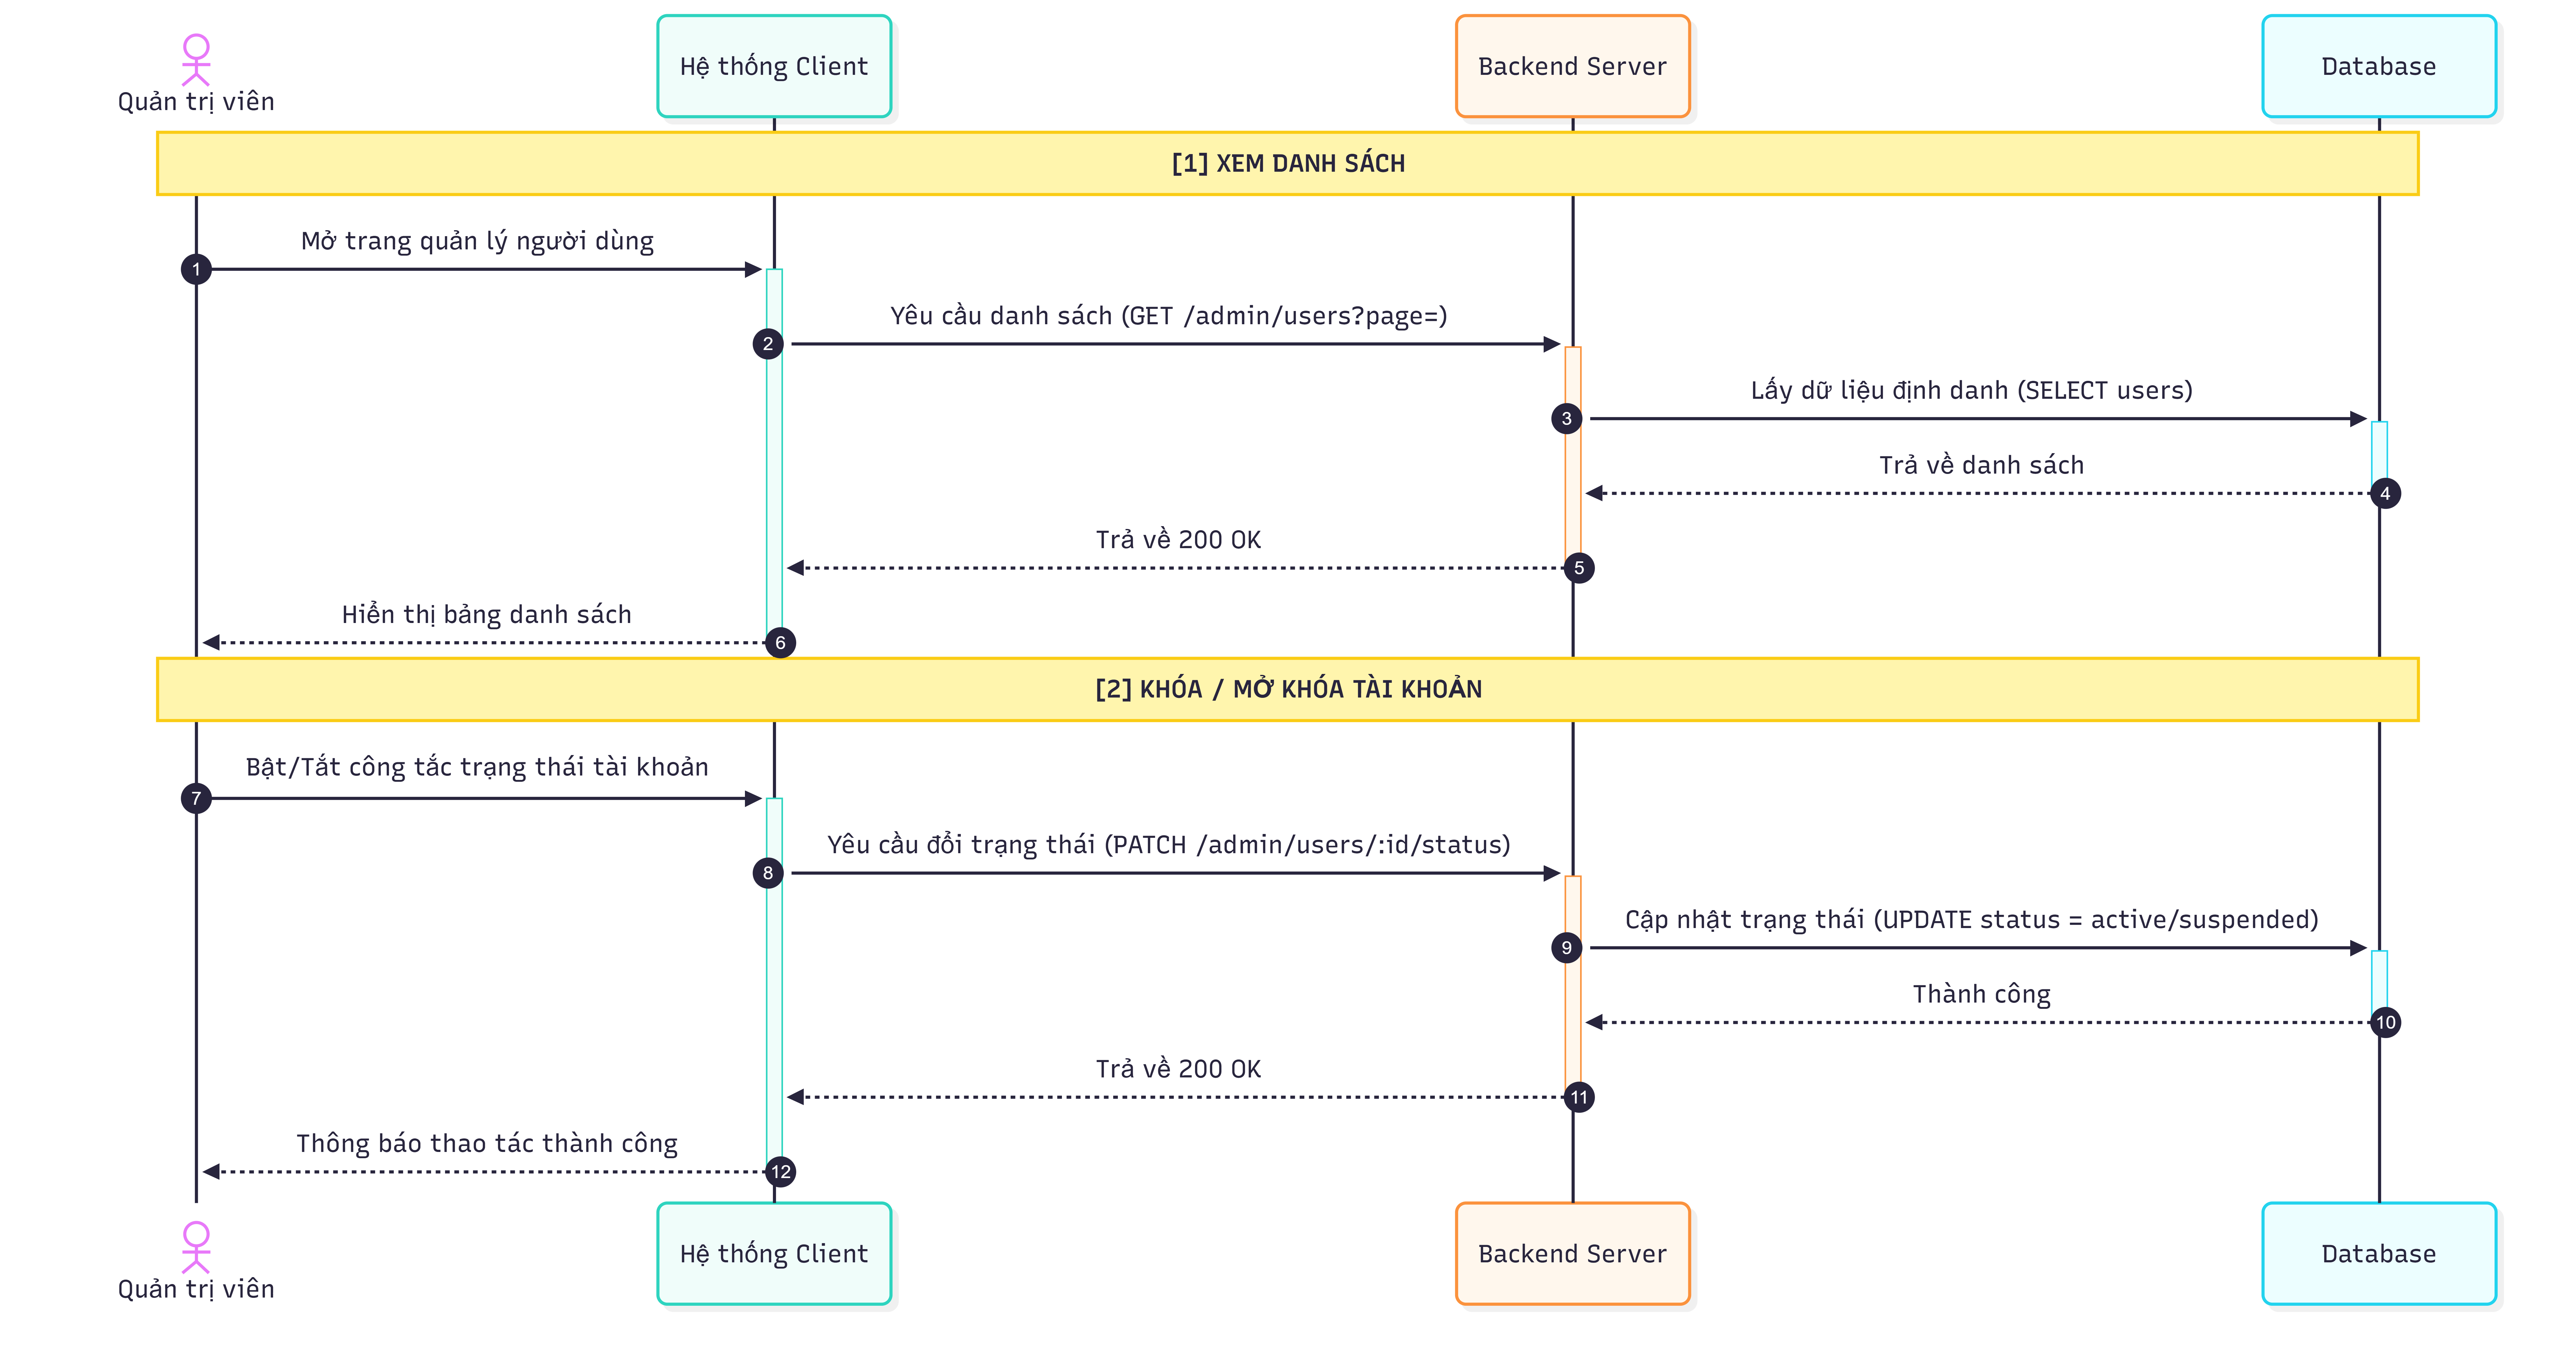
\includegraphics[width=\textwidth,height=0.85\textheight,keepaspectratio]{sd-12-user-management.png}
    \caption{Biểu đồ tuần tự: Quản lý người dùng}
    \label{fig:sd-12}
\end{figure}

\subsection{SD-13: Xử lý phản hồi (Admin)}
% \noindent\textit{[Chèn ảnh SD-13 tại đây]}
\begin{figure}[htbp]
    \centering
    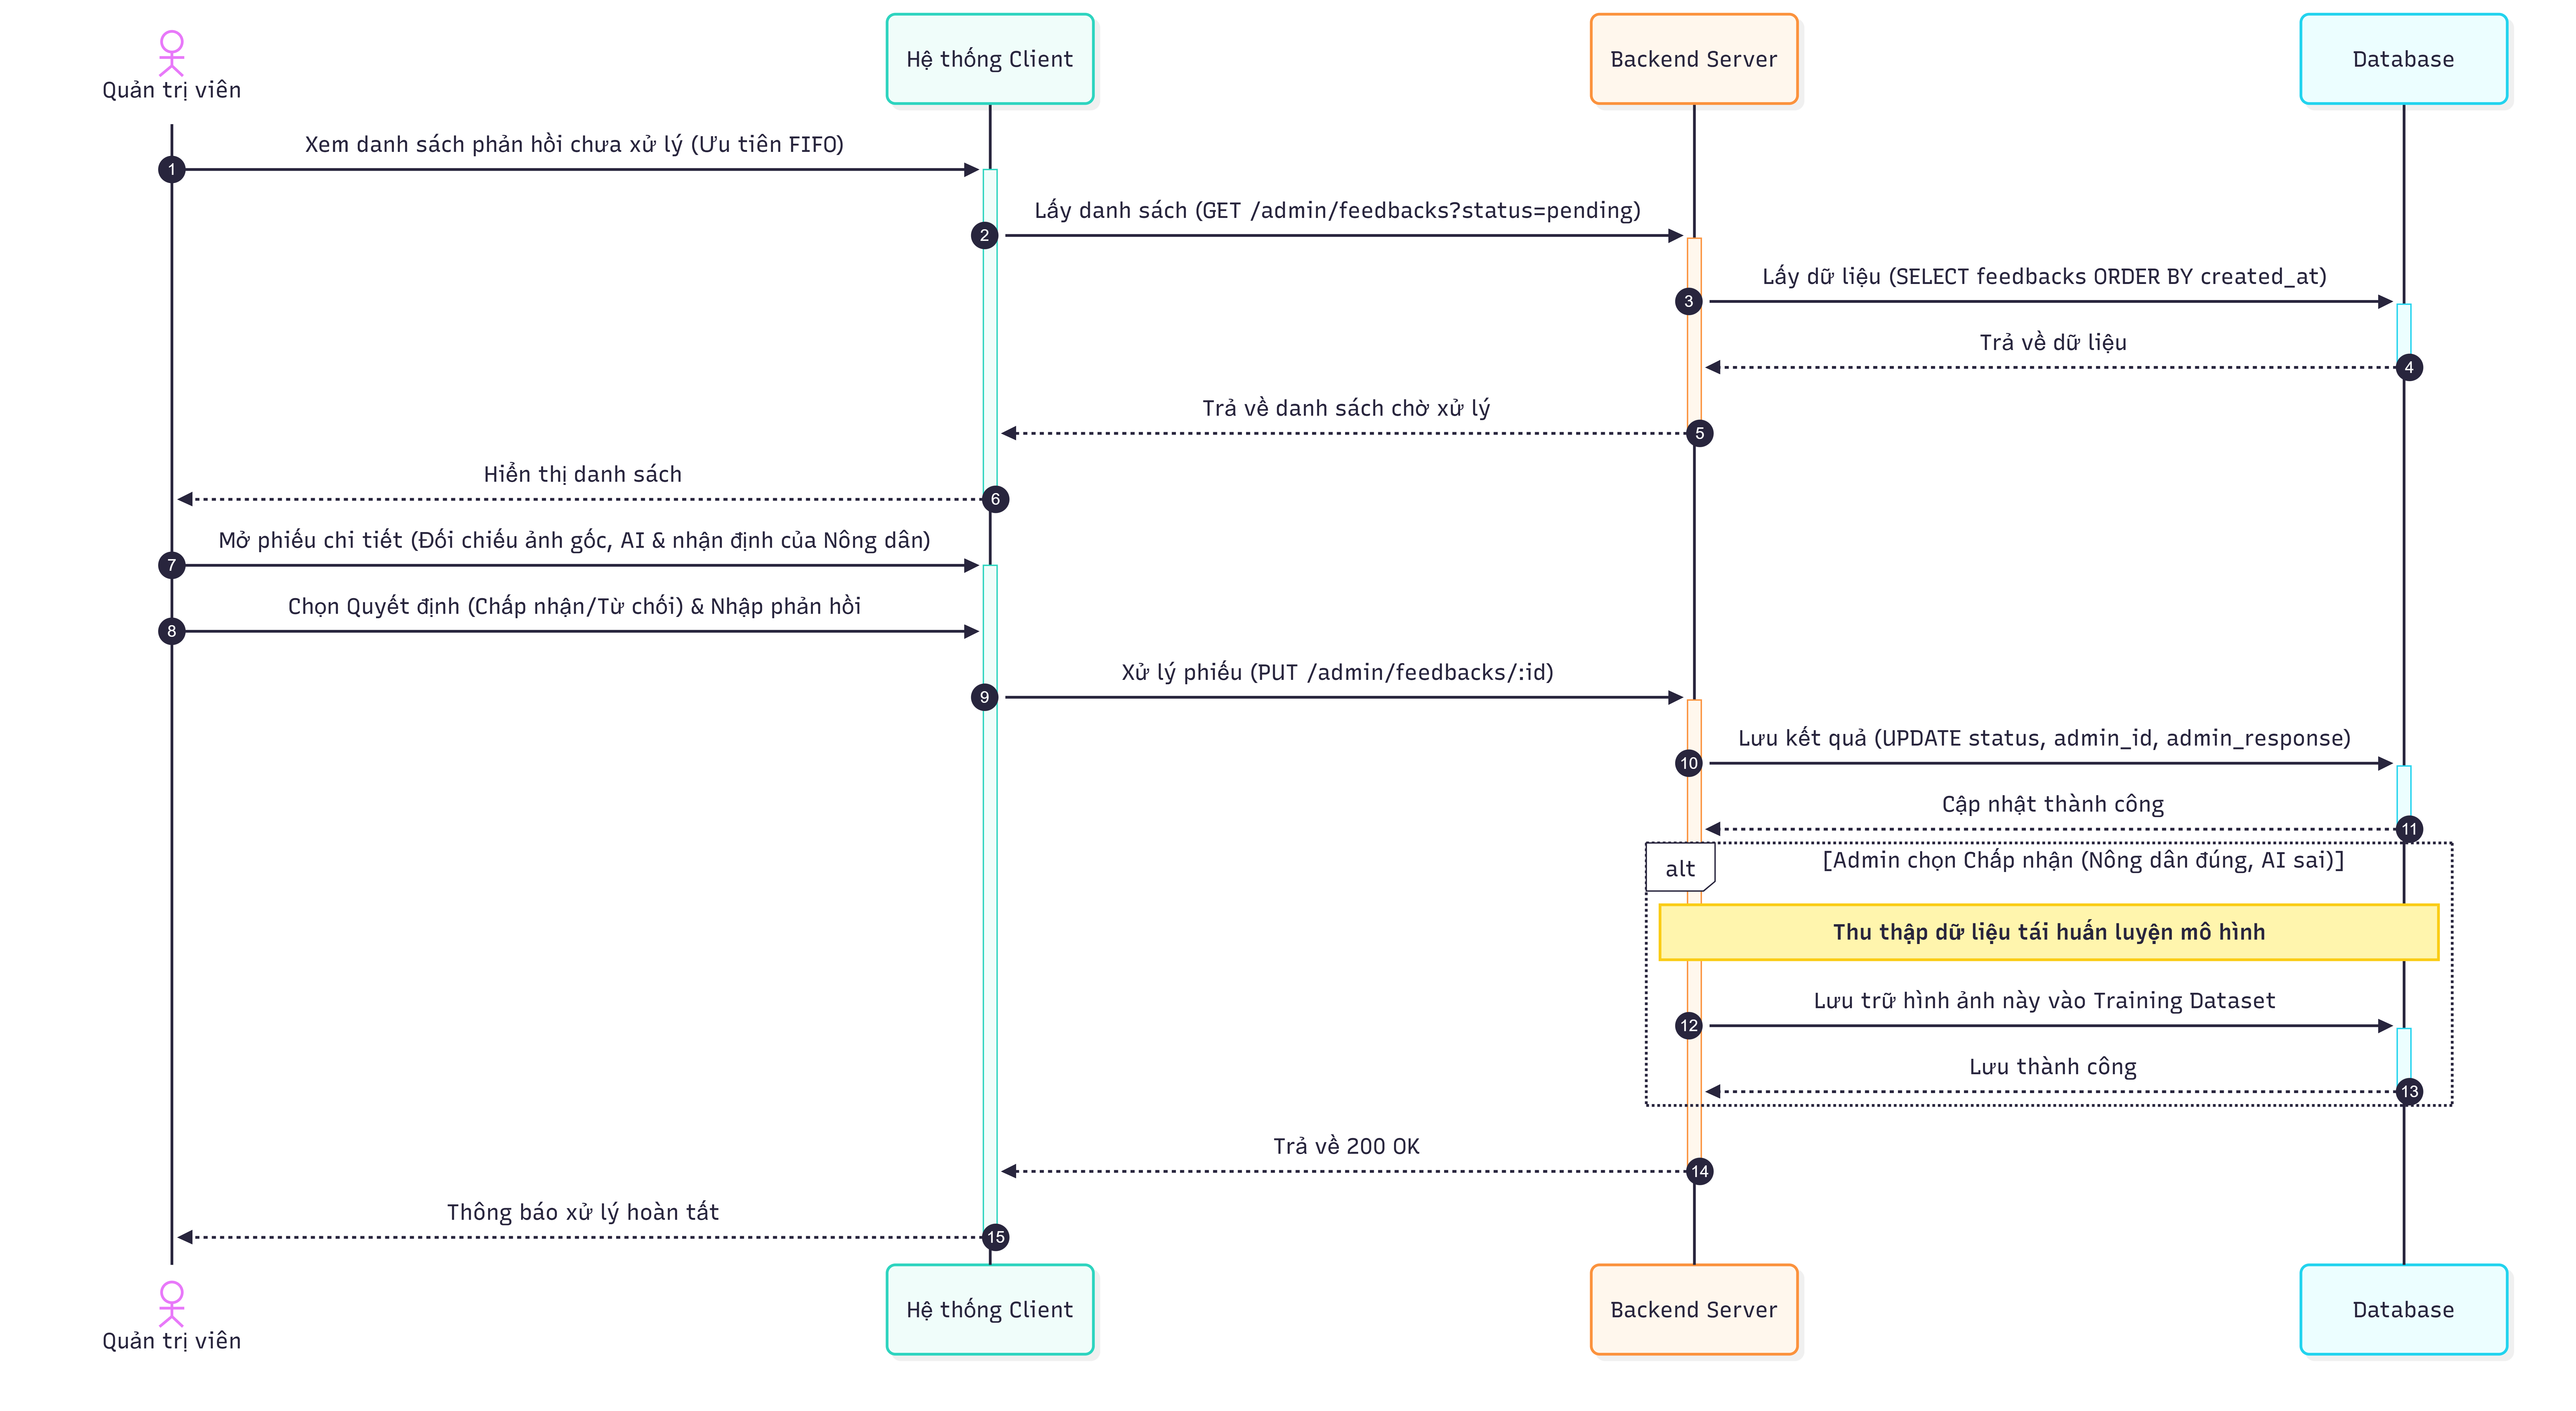
\includegraphics[width=\textwidth,height=0.85\textheight,keepaspectratio]{sd-13-feedback-admin.png}
    \caption{Biểu đồ tuần tự: Xử lý phản hồi (Admin)}
    \label{fig:sd-13}
\end{figure}

\subsection{SD-14: Cập nhật mô hình AI}
% \noindent\textit{[Chèn ảnh SD-14 tại đây]}
\begin{figure}[htbp]
    \centering
    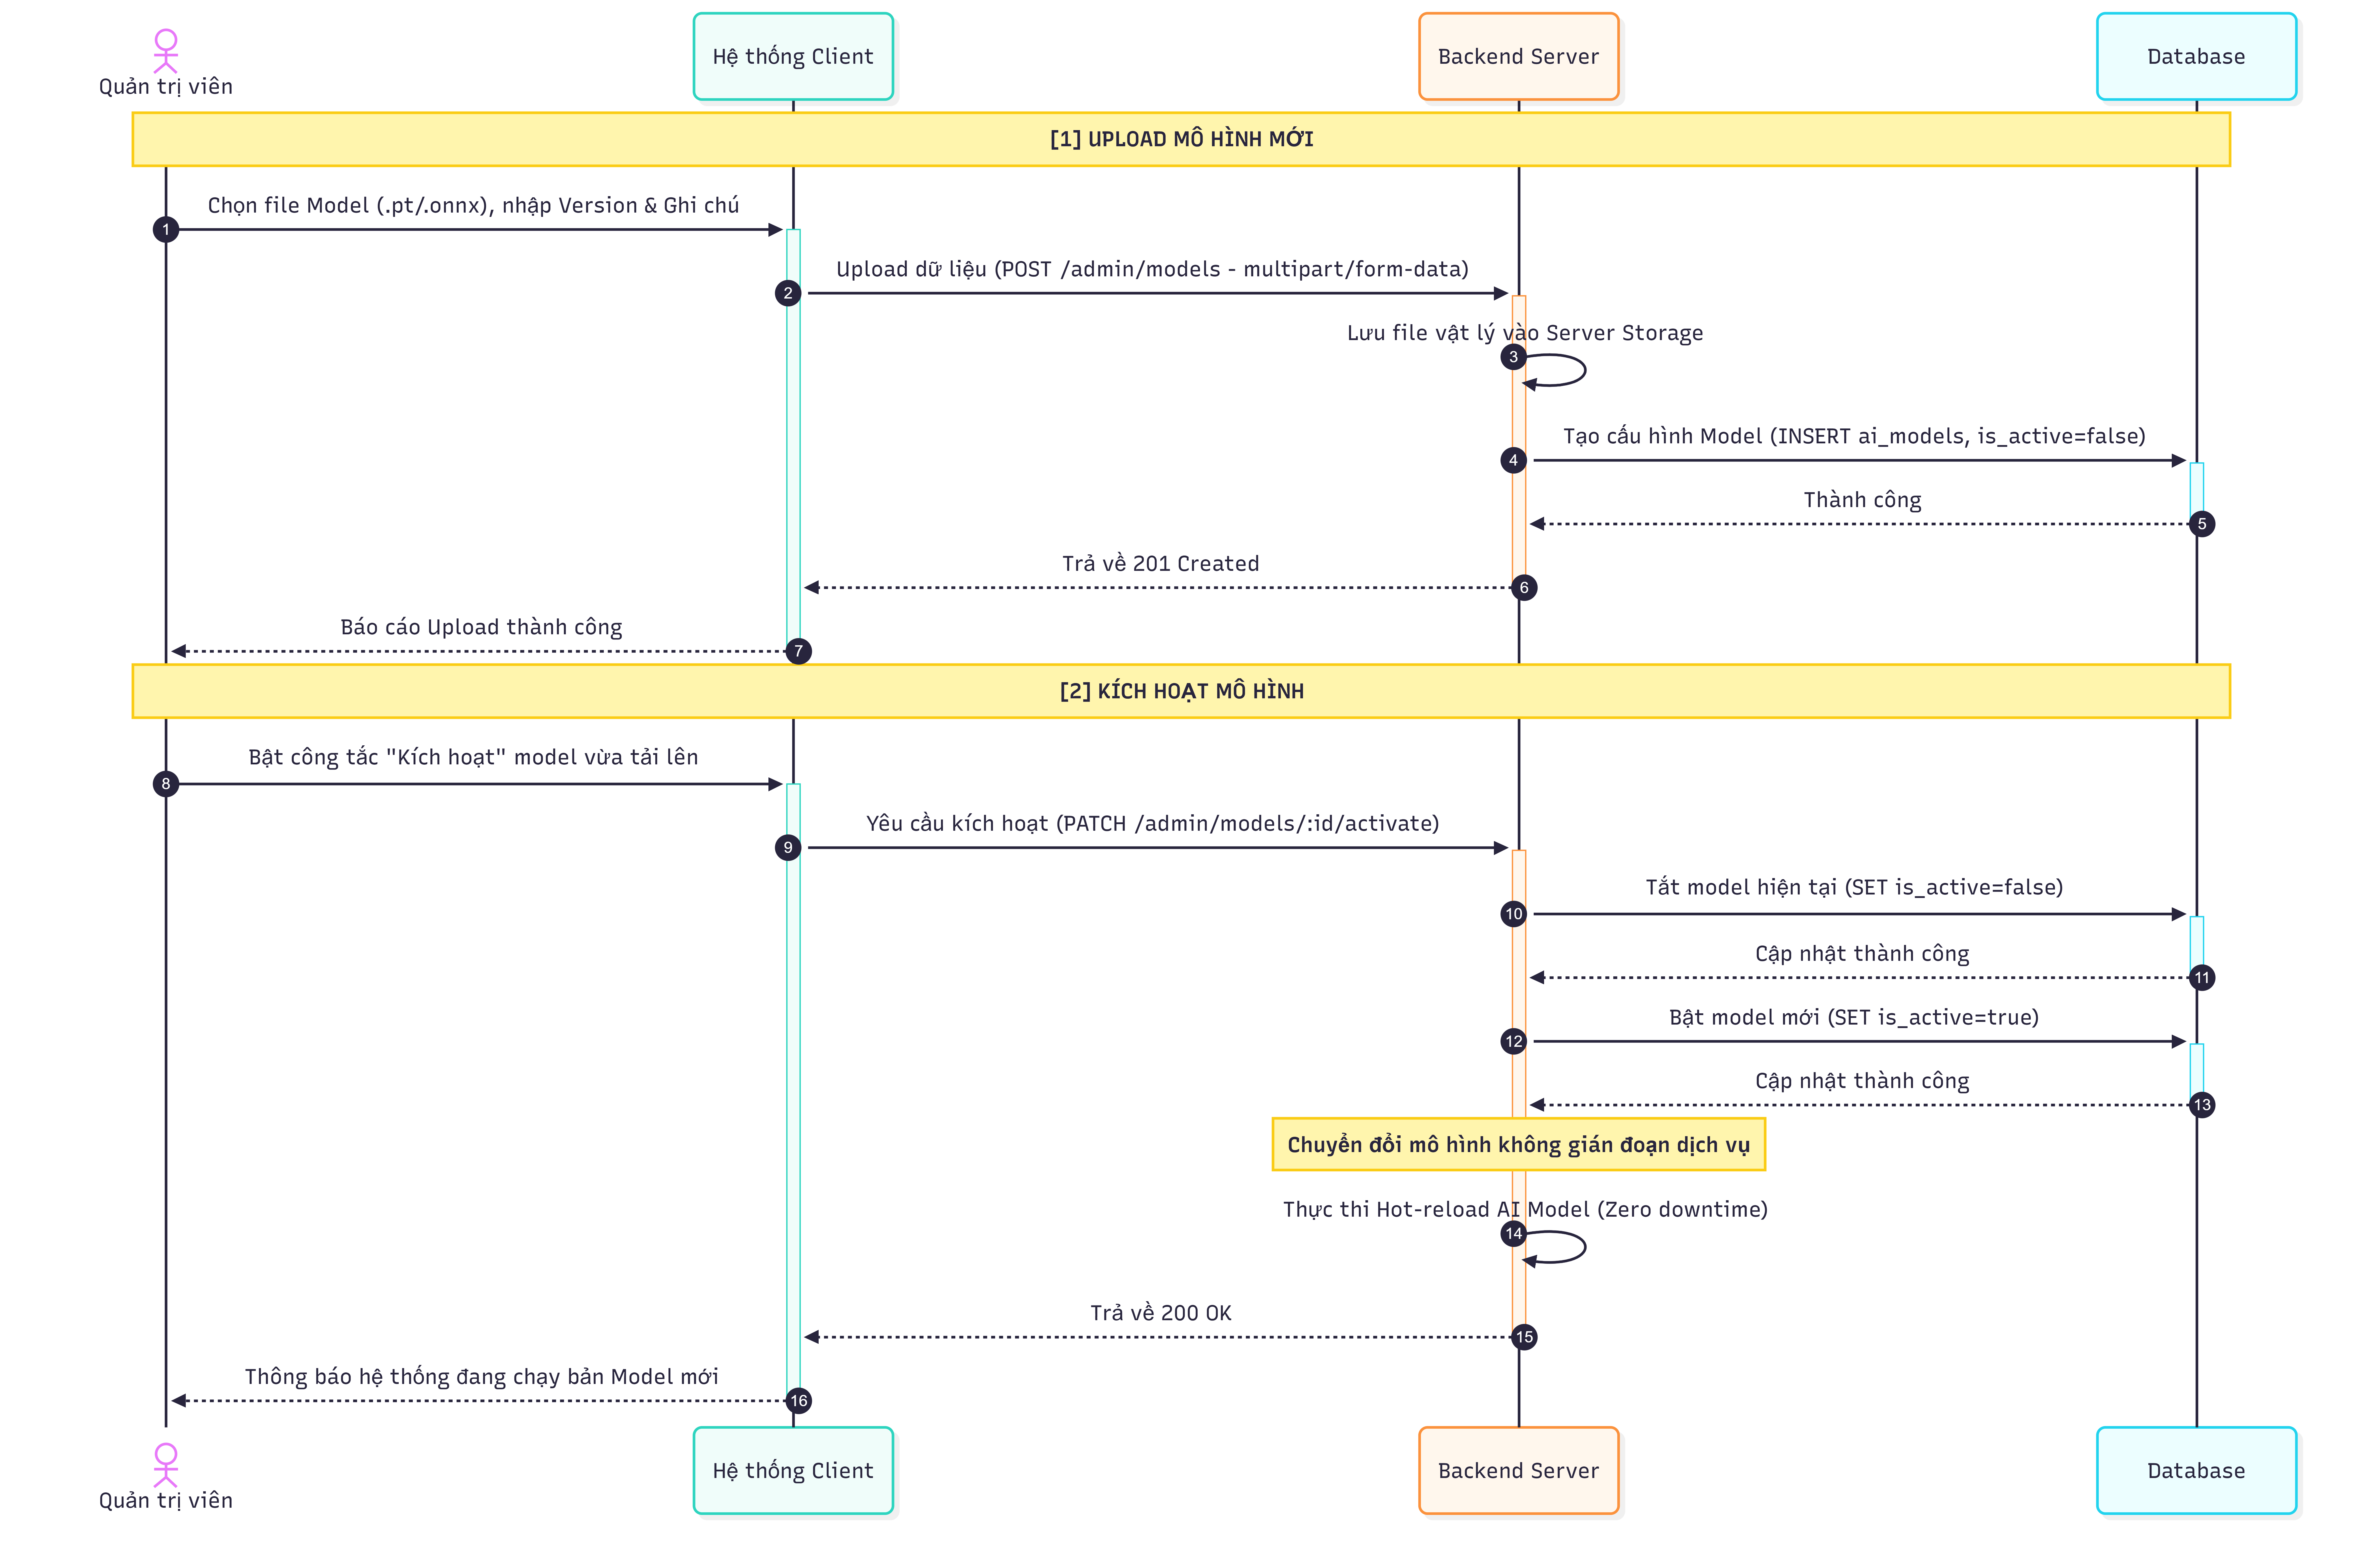
\includegraphics[width=\textwidth,height=0.85\textheight,keepaspectratio]{sd-14-model-update.png}
    \caption{Biểu đồ tuần tự: Cập nhật mô hình AI}
    \label{fig:sd-14}
\end{figure}

\subsection{SD-15: Thống kê \& Báo cáo}
% \noindent\textit{[Chèn ảnh SD-15 tại đây]}
\begin{figure}[htbp]
    \centering
    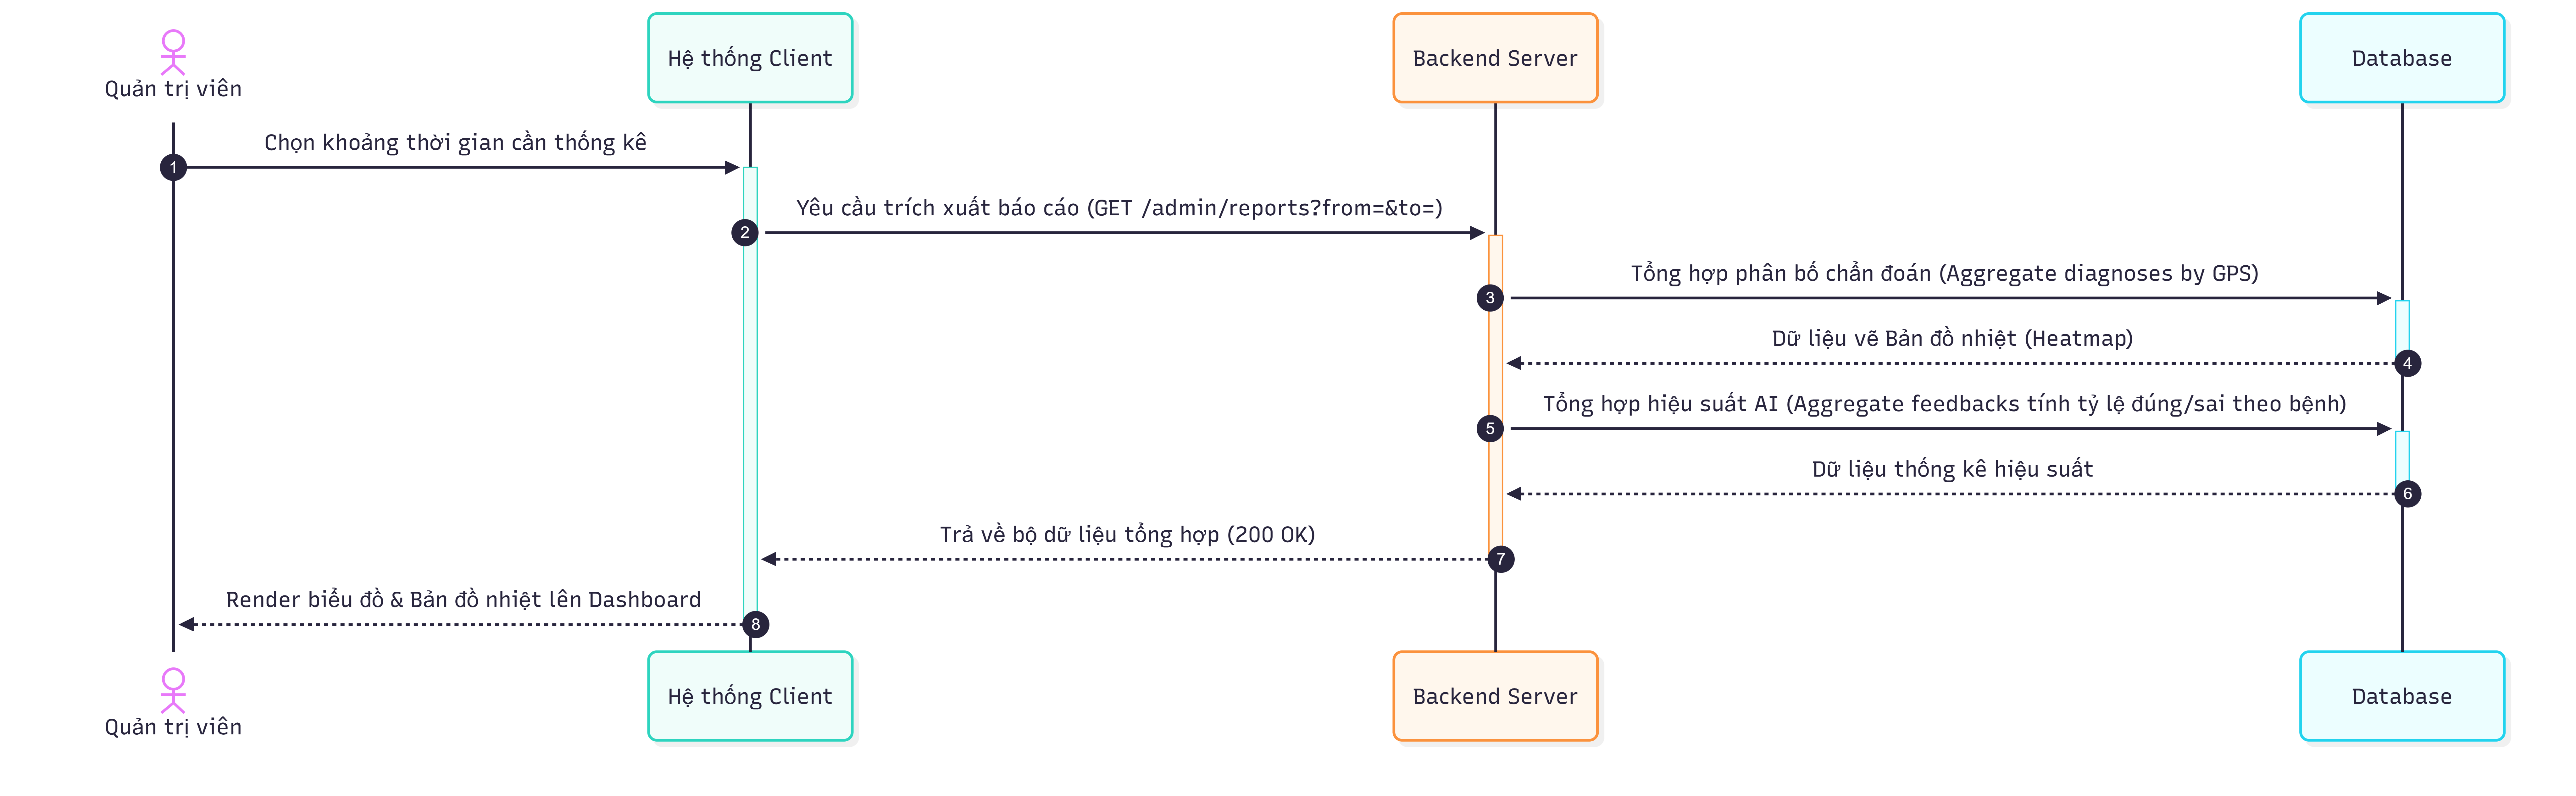
\includegraphics[width=\textwidth,height=0.85\textheight,keepaspectratio]{sd-15-reports.png}
    \caption{Biểu đồ tuần tự: Thống kê và báo cáo}
    \label{fig:sd-15}
\end{figure}

\hrulefill

% ============================================================
\section{Thiết kế Cơ sở dữ liệu}

\subsection{Bảng users}
\begin{longtable}{|l|l|l|p{5cm}|}
    \caption{Cấu trúc bảng users}                                                          \\
    \hline
    \rowcolor{headerblue}
    \textbf{Trường} & \textbf{Kiểu} & \textbf{Ràng buộc}                & \textbf{Ghi chú} \\
    \hline
    id              & UUID          & PK                                &                  \\
    \hline
    username        & VARCHAR(50)   & UNIQUE, NOT NULL                  &                  \\
    \hline
    email           & VARCHAR(255)  & UNIQUE, NOT NULL                  &                  \\
    \hline
    password        & VARCHAR       &                                   & Nullable cho Social Login \\
    \hline
    role            & ENUM          & 'user', 'admin'                   &                  \\
    \hline
    status          & ENUM          & 'active', 'inactive', 'suspended' &                  \\
    \hline
    metadata        & JSONB         &                                   & Cấu hình/thông tin bổ sung \\
    \hline
    created\_at     & TIMESTAMP     & Default now()                     &                  \\
    \hline
    updated\_at     & TIMESTAMP     &                                   &                  \\
    \hline
    \rowcolor{headerblue}
    \textbf{Indexes} & \multicolumn{3}{l|}{username, email}                                \\
    \hline
\end{longtable}

\textit{Lưu ý:} Số lần đăng nhập sai và thời gian khóa tạm thời được lưu trên \textbf{Redis}, không lưu trong CSDL.

\subsection{Bảng user\_profiles}
\begin{longtable}{|l|l|l|p{5.5cm}|}
    \caption{Cấu trúc bảng user\_profiles}                                             \\
    \hline
    \rowcolor{headerblue}
    \textbf{Trường} & \textbf{Kiểu} & \textbf{Ràng buộc}             & \textbf{Ghi chú} \\
    \hline
    id              & UUID          & PK                             &                  \\
    \hline
    user\_id        & FK            & $\rightarrow$ users.id, UNIQUE & Quan hệ 1--1     \\
    \hline
    first\_name     & VARCHAR       &                                & Họ               \\
    \hline
    last\_name      & VARCHAR       &                                & Tên              \\
    \hline
    created\_at     & TIMESTAMP     & Default now()                  &                  \\
    \hline
    updated\_at     & TIMESTAMP     &                                &                  \\
    \hline
    \rowcolor{headerblue}
    \textbf{Indexes} & \multicolumn{3}{l|}{user\_id (Unique FK)}                            \\
    \hline
\end{longtable}

\subsection{Bảng user\_social\_accounts}
\begin{longtable}{|l|l|l|p{5.5cm}|}
    \caption{Cấu trúc bảng user\_social\_accounts}                                                      \\
    \hline
    \rowcolor{headerblue}
    \textbf{Trường}     & \textbf{Kiểu} & \textbf{Ràng buộc}           & \textbf{Ghi chú}        \\
    \hline
    id                  & UUID          & PK                           &                         \\
    \hline
    user\_id            & FK            & $\rightarrow$ users.id       & Quan hệ 1--N            \\
    \hline
    provider            & VARCHAR       & NOT NULL                     & Google, Facebook, v.v.   \\
    \hline
    provider\_user\_id  & VARCHAR       & UNIQUE, NOT NULL             & ID từ nhà cung cấp      \\
    \hline
    created\_at         & TIMESTAMP     & Default now()                &                         \\
    \hline
    updated\_at         & TIMESTAMP     &                              &                         \\
    \hline
    \rowcolor{headerblue}
    \textbf{Indexes}    & \multicolumn{3}{l|}{user\_id, provider, provider\_user\_id, (user\_id, provider)} \\
    \hline
\end{longtable}

\subsection{Bảng diseases}
\begin{longtable}{|l|l|l|p{5.5cm}|}
    \caption{Cấu trúc bảng diseases}                                          \\
    \hline
    \rowcolor{headerblue}
    \textbf{Trường}  & \textbf{Kiểu} & \textbf{Ràng buộc}  & \textbf{Ghi chú} \\
    \hline
    id               & UUID          & PK                  &                  \\
    \hline
    name             & NVARCHAR(100) & UNIQUE, NOT NULL    & Tên tiếng Việt   \\
    \hline
    scientific\_name & VARCHAR(150)  & UNIQUE              & Tên khoa học     \\
    \hline
    signs            & TEXT          &                     & Dấu hiệu bệnh    \\
    \hline
    status           & ENUM          & 'visible', 'hidden' &                  \\
    \hline
    created\_at      & TIMESTAMP     & Default now()       &                  \\
    \hline
    updated\_at      & TIMESTAMP     &                     &                  \\
    \hline
    \rowcolor{headerblue}
    \textbf{Indexes} & \multicolumn{3}{l|}{name, scientific\_name}               \\
    \hline
\end{longtable}

\subsection{Bảng nutritions (Vector Database)}
\begin{longtable}{|l|l|l|p{5.5cm}|}
    \caption{Cấu trúc bảng nutritions}                                                         \\
    \hline
    \rowcolor{headerblue}
    \textbf{Trường} & \textbf{Kiểu} & \textbf{Ràng buộc} & \textbf{Ghi chú}                    \\
    \hline
    id              & UUID          & PK                 &                                     \\
    \hline
    content         & TEXT          & NOT NULL           & Nội dung tri thức                   \\
    \hline
    source          & NVARCHAR(100) &                    & Nguồn tài liệu                      \\
    \hline
    embedding       & VECTOR(1536)  &                    & Vector ngữ nghĩa (pgvector)         \\
    \hline
    chunk\_metadata & JSONB         &                    & Thông tin bổ sung, hỗ trợ GIN Index \\
    \hline
    created\_at     & TIMESTAMP     & Default now()      &                                     \\
    \hline
    updated\_at     & TIMESTAMP     &                    &                                     \\
    \hline
    \rowcolor{headerblue}
    \textbf{Indexes} & \multicolumn{3}{l|}{id (PK)}                                         \\
    \hline
\end{longtable}

\subsection{Bảng diagnoses}
\begin{longtable}{|l|l|l|p{5.5cm}|}
    \caption{Cấu trúc bảng diagnoses}                                                             \\
    \hline
    \rowcolor{headerblue}
    \textbf{Trường}      & \textbf{Kiểu} & \textbf{Ràng buộc}          & \textbf{Ghi chú}         \\
    \hline
    id                   & UUID          & PK                          &                          \\
    \hline
    user\_id             & FK            & $\rightarrow$ users.id      &                          \\
    \hline
    original\_image\_url & VARCHAR(512)  & NOT NULL                    &                          \\
    \hline
    result\_image\_url   & VARCHAR(512)  &                             &                          \\
    \hline
    gps\_lat             & DECIMAL(10,8) &                             & Tọa độ gọi API thời tiết \\
    \hline
    gps\_lng             & DECIMAL(11,8) &                             &                          \\
    \hline
    province             & TEXT          &                             & Tỉnh/thành phố           \\
    \hline
    weather\_data        & JSONB         &                             & Dữ liệu thời tiết từ API \\
    \hline
    env\_description     & TEXT          &                             &                          \\
    \hline
    model\_version\_id   & FK            & $\rightarrow$ ai\_models.id &                          \\
    \hline
    created\_at          & TIMESTAMP     & Default now()               &                          \\
    \hline
    updated\_at          & TIMESTAMP     &                             &                          \\
    \hline
    \rowcolor{headerblue}
    \textbf{Indexes}     & \multicolumn{3}{l|}{user\_id, model\_version\_id}                        \\
    \hline
\end{longtable}

\subsection{Bảng diagnosis\_results (1--N)}
\begin{longtable}{|l|l|l|p{5.5cm}|}
    \caption{Cấu trúc bảng diagnosis\_results}                                                \\
    \hline
    \rowcolor{headerblue}
    \textbf{Trường} & \textbf{Kiểu} & \textbf{Ràng buộc}         & \textbf{Ghi chú}           \\
    \hline
    id              & UUID          & PK                         &                            \\
    \hline
    diagnosis\_id   & FK            & $\rightarrow$ diagnoses.id &                            \\
    \hline
    disease\_id     & FK            & $\rightarrow$ diseases.id  &                            \\
    \hline
    confidence      & DECIMAL(5,2)  & 0--100.00                  & \% độ tin cậy              \\
    \hline
    mask\_polygon   & JSONB         &                            & Tọa độ polygon             \\
    \hline
    color           & VARCHAR(20)   &                            & Màu sắc bounding box       \\
    \hline
    advisory        & JSONB         &                            & Khuyến nghị xử lý          \\
    \hline
    created\_at     & TIMESTAMP     & Default now()              &                            \\
    \hline
    updated\_at     & TIMESTAMP     &                            &                            \\
    \hline
    \rowcolor{headerblue}
    \textbf{Indexes} & \multicolumn{3}{l|}{diagnosis\_id, disease\_id}                          \\
    \hline
\end{longtable}

\subsection{Bảng feedbacks}
\clearpage
\begin{table}[htbp]
    \centering
    \small
    \renewcommand{\arraystretch}{0.95}
    \setlength{\tabcolsep}{5pt}
    \caption{Cấu trúc bảng feedbacks}
    \begin{tabular}{|l|l|l|p{5.5cm}|}
        \hline
        \rowcolor{headerblue}
        \textbf{Trường} & \textbf{Kiểu} & \textbf{Ràng buộc}                & \textbf{Ghi chú}       \\
        \hline
        id              & UUID          & PK                                &                        \\
        \hline
        diagnosis\_id   & FK            & $\rightarrow$ diagnoses.id        &                        \\
        \hline
        user\_id        & FK            & $\rightarrow$ users.id            & Người gửi              \\
        \hline
        user\_message   & TEXT          &                                   & Lời nhắn nông dân      \\
        \hline
        status          & ENUM          & 'pending', 'accepted', 'rejected' &                        \\
        \hline
        admin\_id       & FK            & $\rightarrow$ users.id, nullable  & Admin xử lý            \\
        \hline
        admin\_response & TEXT          &                                   & Lời nhắn admin gửi lại \\
        \hline
        processed\_at   & TIMESTAMP     &                                   &                        \\
        \hline
        created\_at     & TIMESTAMP     & Default now()                     &                        \\
        \hline
        updated\_at     & TIMESTAMP     &                                   &                        \\
        \hline
        \rowcolor{headerblue}
        \textbf{Indexes} & \multicolumn{3}{l|}{diagnosis\_id, user\_id, status}                      \\
        \hline
    \end{tabular}
\end{table}

\subsection{Bảng feedback\_actual\_diseases (Junction)}
\begin{longtable}{|l|l|l|p{5.5cm}|}
    \caption{Cấu trúc bảng feedback\_actual\_diseases}                                \\
    \hline
    \rowcolor{headerblue}
    \textbf{Trường} & \textbf{Kiểu} & \textbf{Ràng buộc} & \textbf{Ghi chú}           \\
    \hline
    feedback\_id    & UUID          & PK, FK             & $\rightarrow$ feedbacks.id \\
    \hline
    disease\_id     & UUID          & PK, FK             & $\rightarrow$ diseases.id  \\
    \hline
    created\_at     & TIMESTAMP     & Default now()      &                            \\
    \hline
    updated\_at     & TIMESTAMP     &                    &                            \\
    \hline
    \rowcolor{headerblue}
    \textbf{Indexes} & \multicolumn{3}{l|}{(feedback\_id, disease\_id) [PK]}          \\
    \hline
\end{longtable}

\subsection{Bảng ai\_models}
\begin{longtable}{|l|l|l|p{5.5cm}|}
    \caption{Cấu trúc bảng ai\_models}                                          \\
    \hline
    \rowcolor{headerblue}
    \textbf{Trường} & \textbf{Kiểu} & \textbf{Ràng buộc}     & \textbf{Ghi chú} \\
    \hline
    id              & UUID          & PK                     &                  \\
    \hline
    version\_name   & NVARCHAR(50)  & NOT NULL               & Tên phiên bản    \\
    \hline
    file\_path      & VARCHAR(512)  & NOT NULL               & Đường dẫn file   \\
    \hline
    release\_notes  & TEXT          &                        & Ghi chú thay đổi \\
    \hline
    is\_active      & BOOLEAN       & Default false          & Chỉ 1 active     \\
    \hline
    uploaded\_by    & FK            & $\rightarrow$ users.id & Admin upload     \\
    \hline
    created\_at     & TIMESTAMP     & Default now()          &                  \\
    \hline
    updated\_at     & TIMESTAMP     &                        &                  \\
    \hline
    \rowcolor{headerblue}
    \textbf{Indexes} & \multicolumn{3}{l|}{id (PK)}                                \\
    \hline
\end{longtable}

\subsection{Redis Keys}
\begin{longtable}{|l|p{7.5cm}|l|}
    \caption{Các pattern key trong Redis}                                              \\
    \hline
    \rowcolor{headerblue}
    \textbf{Key Pattern}    & \textbf{Mô tả}        & \textbf{TTL}                     \\
    \hline
    login:fail:\{username\} & Số lần đăng nhập sai  & 15 phút (user) / 30 phút (admin) \\
    \hline
    otp:\{email\}           & OTP 6 số + số lần thử & 10 phút                          \\
    \hline
    verify:\{token\}        & Token xác thực email  & 24 giờ                           \\
    \hline
\end{longtable}

\subsection{Sơ đồ quan hệ thực thể (ERD)}

% \noindent\textit{[Chèn ảnh ER Diagram tại đây --- sinh từ db.dbml]}
\begin{figure}[htbp]
    \centering
    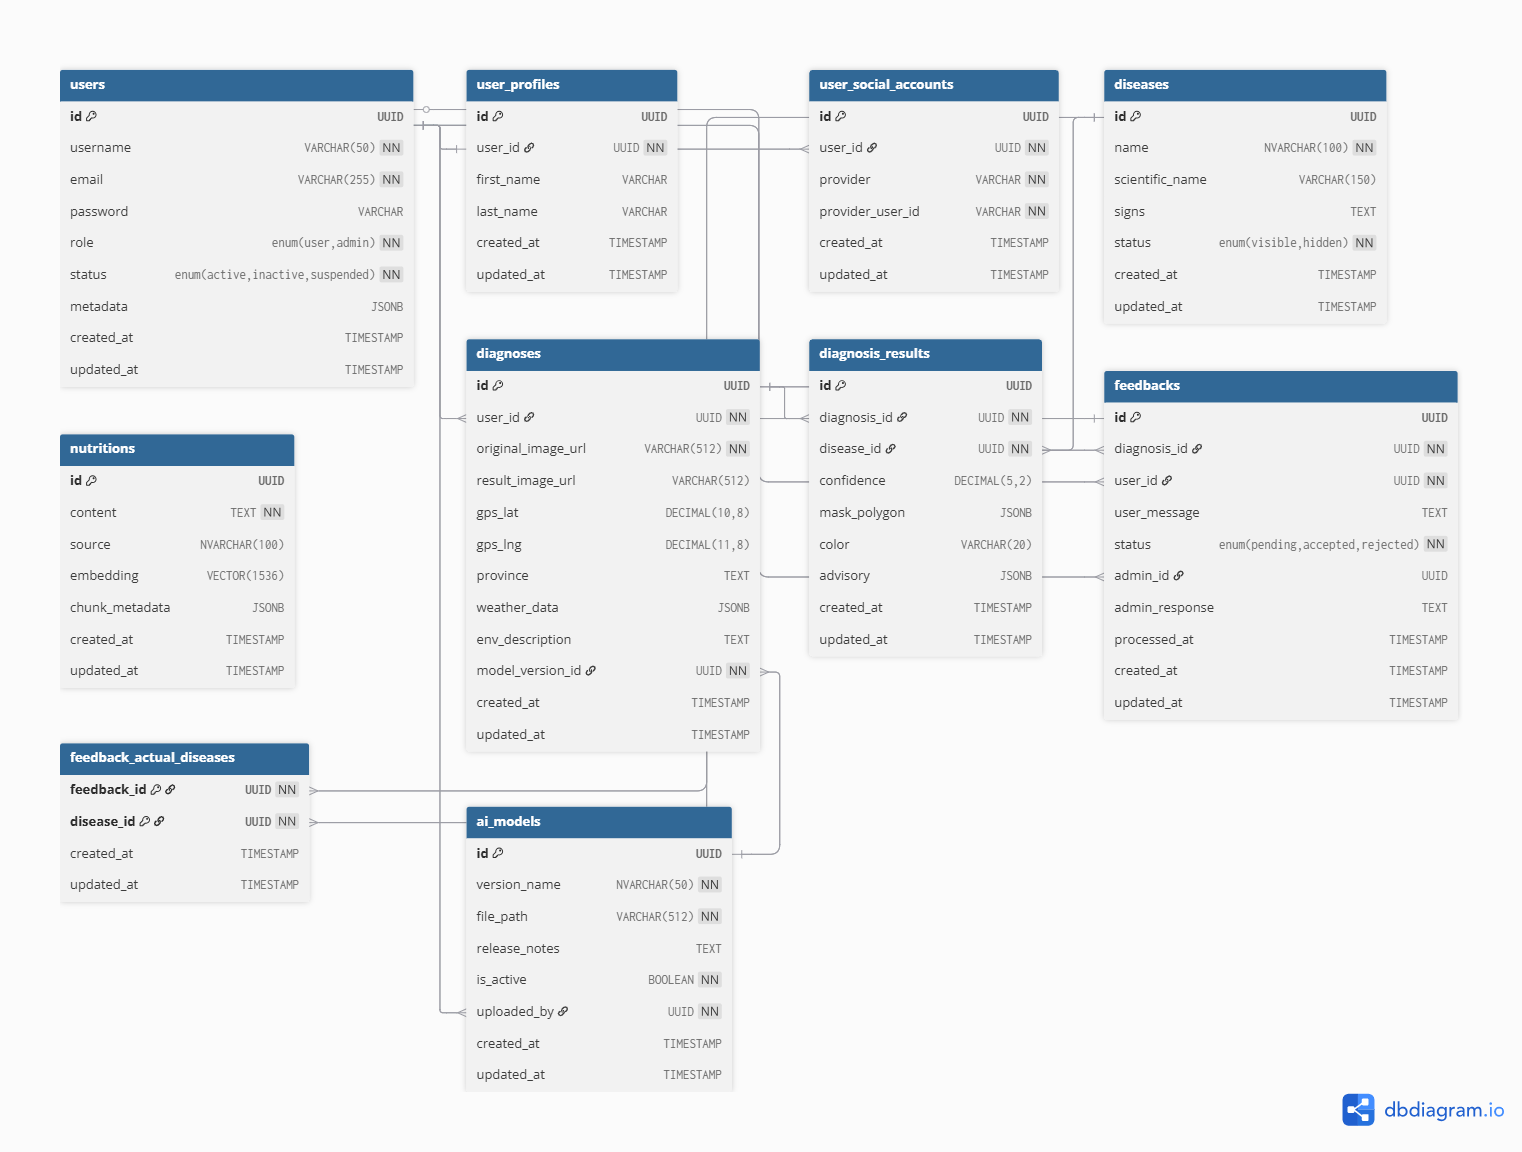
\includegraphics[width=\textwidth,height=0.85\textheight,keepaspectratio]{erd.png}
    \caption{Sơ đồ quan hệ thực thể (ERD)}
    \label{fig:erd}
\end{figure}

\hrulefill

% ============================================================
\section{Giải thích thuật ngữ}

\begin{longtable}{|l|p{11.5cm}|}
    \caption{Giải thích các thuật ngữ chuyên ngành}                                                           \\
    \hline
    \rowcolor{headerblue}
    \textbf{Thuật ngữ}    & \textbf{Giải thích}                                                               \\
    \hline
    CNN                   & Mạng nơ-ron tích chập --- thuật toán AI chuyên phân tích hình ảnh.                \\
    \hline
    Instance Segmentation & Kỹ thuật AI khoanh vùng chính xác từng đối tượng bệnh trên ảnh (pixel-level).     \\
    \hline
    pgvector              & Phần mở rộng của PostgreSQL cho phép tìm kiếm ngữ nghĩa trên dữ liệu văn bản.     \\
    \hline
    Embedding             & Biểu diễn số của văn bản để máy hiểu nghĩa, phục vụ tìm kiếm thông minh.          \\
    \hline
    RAG                   & Retrieval-Augmented Generation --- truy xuất tri thức để AI tư vấn chính xác hơn. \\
    \hline
    Redis                 & Bộ nhớ đệm tốc độ cao, dùng lưu tạm OTP và đếm lần đăng nhập sai.                 \\
    \hline
    JWT                   & Mã thông báo xác thực, giữ trạng thái đăng nhập của người dùng.                   \\
    \hline
    Bcrypt                & Thuật toán mã hóa mật khẩu một chiều, không thể giải ngược.                       \\
    \hline
    OTP                   & Mã xác thực dùng một lần, gửi qua email, hết hạn sau 10 phút.                     \\
    \hline
    GPS                   & Hệ thống định vị toàn cầu, xác định tọa độ vị trí người dùng.                     \\
    \hline
    Hot-swap              & Thay thế mô hình AI mà không cần tắt hệ thống.                                    \\
    \hline
    ERD                   & Sơ đồ thực thể quan hệ --- mô tả cấu trúc và quan hệ giữa các bảng dữ liệu.       \\
    \hline
    mask\_polygon         & Mảng tọa độ đa giác mô tả đường viền vùng bệnh trên ảnh.                          \\
    \hline
\end{longtable}

\end{document}
